\batchmode
\documentclass[onecolumn,11pt]{report}
\RequirePackage{ifthen}


\usepackage{graphicx}    
\topmargin -1.5cm        % read Lamport p.163
\oddsidemargin -0.04cm   % read Lamport p.163
\evensidemargin -0.04cm  % same as oddsidemargin but for left-hand pages
\textwidth 16.59cm
\textheight 21.94cm 
\parskip 7.2pt           % sets spacing between paragraphs
\parindent 0pt		 
\usepackage{authblk}
\usepackage{mathtools}
\usepackage{amsmath}
\usepackage{amssymb}
\usepackage{ulem}
\usepackage{float}
\usepackage{hyperref}
\usepackage{color,soul}


\usepackage[latin1]{inputenc}



\makeatletter

\makeatletter
\count@=\the\catcode`\_ \catcode`\_=8 
\newenvironment{tex2html_wrap}{}{}%
\catcode`\<=12\catcode`\_=\count@
\newcommand{\providedcommand}[1]{\expandafter\providecommand\csname #1\endcsname}%
\newcommand{\renewedcommand}[1]{\expandafter\providecommand\csname #1\endcsname{}%
  \expandafter\renewcommand\csname #1\endcsname}%
\newcommand{\newedenvironment}[1]{\newenvironment{#1}{}{}\renewenvironment{#1}}%
\let\newedcommand\renewedcommand
\let\renewedenvironment\newedenvironment
\makeatother
\let\mathon=$
\let\mathoff=$
\ifx\AtBeginDocument\undefined \newcommand{\AtBeginDocument}[1]{}\fi
\newbox\sizebox
\setlength{\hoffset}{0pt}\setlength{\voffset}{0pt}
\addtolength{\textheight}{\footskip}\setlength{\footskip}{0pt}
\addtolength{\textheight}{\topmargin}\setlength{\topmargin}{0pt}
\addtolength{\textheight}{\headheight}\setlength{\headheight}{0pt}
\addtolength{\textheight}{\headsep}\setlength{\headsep}{0pt}
\setlength{\textwidth}{349pt}
\newwrite\lthtmlwrite
\makeatletter
\let\realnormalsize=\normalsize
\global\topskip=2sp
\def\preveqno{}\let\real@float=\@float \let\realend@float=\end@float
\def\@float{\let\@savefreelist\@freelist\real@float}
\def\liih@math{\ifmmode$\else\bad@math\fi}
\def\end@float{\realend@float\global\let\@freelist\@savefreelist}
\let\real@dbflt=\@dbflt \let\end@dblfloat=\end@float
\let\@largefloatcheck=\relax
\let\if@boxedmulticols=\iftrue
\def\@dbflt{\let\@savefreelist\@freelist\real@dbflt}
\def\adjustnormalsize{\def\normalsize{\mathsurround=0pt \realnormalsize
 \parindent=0pt\abovedisplayskip=0pt\belowdisplayskip=0pt}%
 \def\phantompar{\csname par\endcsname}\normalsize}%
\def\lthtmltypeout#1{{\let\protect\string \immediate\write\lthtmlwrite{#1}}}%
\usepackage[tightpage,active]{preview}
\newbox\lthtmlPageBox
\newdimen\lthtmlCropMarkHeight
\newdimen\lthtmlCropMarkDepth
\long\def\lthtmlTightVBox#1#2{%
    \setbox\lthtmlPageBox\vbox{\hbox{\catcode`\_=8 #2}}%
    \lthtmlCropMarkHeight=\ht\lthtmlPageBox \advance \lthtmlCropMarkHeight 6pt
    \lthtmlCropMarkDepth=\dp\lthtmlPageBox
    \lthtmltypeout{^^J:#1:lthtmlCropMarkHeight:=\the\lthtmlCropMarkHeight}%
    \lthtmltypeout{^^J:#1:lthtmlCropMarkDepth:=\the\lthtmlCropMarkDepth:1ex:=\the \dimexpr 1ex}%
    \begin{preview}\copy\lthtmlPageBox\end{preview}}}%
\long\def\lthtmlTightFBox#1#2{%
    \adjustnormalsize\setbox\lthtmlPageBox=\vbox\bgroup %
    \let\ifinner=\iffalse \let\)\liih@math %
    {\catcode`\_=8 #2}%
    \@next\next\@currlist{}{\def\next{\voidb@x}}%
    \expandafter\box\next\egroup %
    \lthtmlCropMarkHeight=\ht\lthtmlPageBox \advance \lthtmlCropMarkHeight 6pt
    \lthtmlCropMarkDepth=\dp\lthtmlPageBox
    \lthtmltypeout{^^J:#1:lthtmlCropMarkHeight:=\the\lthtmlCropMarkHeight}%
    \lthtmltypeout{^^J:#1:lthtmlCropMarkDepth:=\the\lthtmlCropMarkDepth:1ex:=\the \dimexpr 1ex}%
    \begin{preview}\copy\lthtmlPageBox\end{preview}}%
    \long\def\lthtmlinlinemathA#1#2\lthtmlindisplaymathZ{\lthtmlTightVBox{#1}{#2}}
    \def\lthtmlinlineA#1#2\lthtmlinlineZ{\lthtmlTightVBox{#1}{#2}}
    \long\def\lthtmldisplayA#1#2\lthtmldisplayZ{\lthtmlTightVBox{#1}{#2}}
    \long\def\lthtmlinlinemathA#1#2\lthtmlindisplaymathZ{\lthtmlTightVBox{#1}{#2}}
    \def\lthtmlinlineA#1#2\lthtmlinlineZ{\lthtmlTightVBox{#1}{#2}}
    \long\def\lthtmldisplayA#1#2\lthtmldisplayZ{\lthtmlTightVBox{#1}{#2}}
    \long\def\lthtmldisplayB#1#2\lthtmldisplayZ{\\edef\preveqno{(\theequation)}%
        \lthtmlTightVBox{#1}{\let\@eqnnum\relax#2}}
    \long\def\lthtmlfigureA#1#2\lthtmlfigureZ{\let\@savefreelist\@freelist
        \lthtmlTightFBox{#1}{#2}\global\let\@freelist\@savefreelist}
    \long\def\lthtmlpictureA#1#2\lthtmlpictureZ{\let\@savefreelist\@freelist
        \lthtmlTightVBox{#1}{#2}\global\let\@freelist\@savefreelist}
\def\lthtmlcheckvsize{\ifdim\ht\sizebox<\vsize 
  \ifdim\wd\sizebox<\hsize\expandafter\hfill\fi \expandafter\vfill
  \else\expandafter\vss\fi}%
\providecommand{\selectlanguage}[1]{}%
\makeatletter \tracingstats = 1 
\providecommand{\omicron}{\textrm{o}}
\providecommand{\Tau}{\textrm{T}}
\providecommand{\Mu}{\textrm{M}}
\providecommand{\Kappa}{\textrm{K}}
\providecommand{\Rho}{\textrm{R}}
\providecommand{\Chi}{\textrm{X}}
\providecommand{\Iota}{\textrm{J}}
\providecommand{\Epsilon}{\textrm{E}}
\providecommand{\Alpha}{\textrm{A}}
\providecommand{\Beta}{\textrm{B}}
\providecommand{\Nu}{\textrm{N}}
\providecommand{\Omicron}{\textrm{O}}
\providecommand{\Eta}{\textrm{H}}
\providecommand{\Zeta}{\textrm{Z}}


\begin{document}
\pagestyle{empty}\thispagestyle{empty}\lthtmltypeout{}%
\lthtmltypeout{latex2htmlLength hsize=\the\hsize}\lthtmltypeout{}%
\lthtmltypeout{latex2htmlLength vsize=\the\vsize}\lthtmltypeout{}%
\lthtmltypeout{latex2htmlLength hoffset=\the\hoffset}\lthtmltypeout{}%
\lthtmltypeout{latex2htmlLength voffset=\the\voffset}\lthtmltypeout{}%
\lthtmltypeout{latex2htmlLength topmargin=\the\topmargin}\lthtmltypeout{}%
\lthtmltypeout{latex2htmlLength topskip=\the\topskip}\lthtmltypeout{}%
\lthtmltypeout{latex2htmlLength headheight=\the\headheight}\lthtmltypeout{}%
\lthtmltypeout{latex2htmlLength headsep=\the\headsep}\lthtmltypeout{}%
\lthtmltypeout{latex2htmlLength parskip=\the\parskip}\lthtmltypeout{}%
\lthtmltypeout{latex2htmlLength oddsidemargin=\the\oddsidemargin}\lthtmltypeout{}%
\makeatletter
\if@twoside\lthtmltypeout{latex2htmlLength evensidemargin=\the\evensidemargin}%
\else\lthtmltypeout{latex2htmlLength evensidemargin=\the\oddsidemargin}\fi%
\lthtmltypeout{}%
\makeatother
\setcounter{page}{1}
\onecolumn

% !!! IMAGES START HERE !!!

{\newpage\clearpage
\lthtmlinlinemathA{tex2html_wrap_inline20515}%
$ P_p$%
\lthtmlindisplaymathZ
\lthtmlcheckvsize\clearpage}

{\newpage\clearpage
\lthtmlinlinemathA{tex2html_wrap_inline20517}%
$ S_v$%
\lthtmlindisplaymathZ
\lthtmlcheckvsize\clearpage}

{\newpage\clearpage
\lthtmlinlinemathA{tex2html_wrap_inline20519}%
$ \sigma _v$%
\lthtmlindisplaymathZ
\lthtmlcheckvsize\clearpage}

{\newpage\clearpage
\lthtmlinlinemathA{tex2html_wrap_inline20525}%
$ S_3$%
\lthtmlindisplaymathZ
\lthtmlcheckvsize\clearpage}

{\newpage\clearpage
\lthtmlinlinemathA{tex2html_wrap_inline20533}%
$ S_{Hmax}$%
\lthtmlindisplaymathZ
\lthtmlcheckvsize\clearpage}

{\newpage\clearpage
\lthtmlinlinemathA{tex2html_wrap_inline20551}%
$ S_{ij}$%
\lthtmlindisplaymathZ
\lthtmlcheckvsize\clearpage}

{\newpage\clearpage
\lthtmlinlinemathA{tex2html_wrap_inline20553}%
$ \uline {e}_i$%
\lthtmlindisplaymathZ
\lthtmlcheckvsize\clearpage}

{\newpage\clearpage
\lthtmlinlinemathA{tex2html_wrap_inline20555}%
$ \uline {e}_j$%
\lthtmlindisplaymathZ
\lthtmlcheckvsize\clearpage}

{\newpage\clearpage
\lthtmlinlinemathA{tex2html_wrap_inline20559}%
$ dx_i$%
\lthtmlindisplaymathZ
\lthtmlcheckvsize\clearpage}

{\newpage\clearpage
\lthtmlinlinemathA{tex2html_wrap_inline20571}%
$ S_{21}$%
\lthtmlindisplaymathZ
\lthtmlcheckvsize\clearpage}

{\newpage\clearpage
\lthtmlinlinemathA{tex2html_wrap_inline20573}%
$ S_{31}+\frac  {\partial S_{31}}{\partial x_3} dx_3$%
\lthtmlindisplaymathZ
\lthtmlcheckvsize\clearpage}

{\newpage\clearpage
\lthtmlinlinemathA{tex2html_wrap_inline20575}%
$ S_{11}+\frac  {\partial S_{11}}{\partial x_1} dx_1$%
\lthtmlindisplaymathZ
\lthtmlcheckvsize\clearpage}

{\newpage\clearpage
\lthtmlinlinemathA{tex2html_wrap_inline20579}%
$ S_{33}$%
\lthtmlindisplaymathZ
\lthtmlcheckvsize\clearpage}

{\newpage\clearpage
\lthtmlinlinemathA{tex2html_wrap_inline20587}%
$ M$%
\lthtmlindisplaymathZ
\lthtmlcheckvsize\clearpage}

{\newpage\clearpage
\lthtmlinlinemathA{tex2html_wrap_inline20591}%
$ E_{load} < E_{unload}$%
\lthtmlindisplaymathZ
\lthtmlcheckvsize\clearpage}

{\newpage\clearpage
\lthtmlinlinemathA{tex2html_wrap_inline20601}%
$ \varepsilon _{Hmax}$%
\lthtmlindisplaymathZ
\lthtmlcheckvsize\clearpage}

{\newpage\clearpage
\lthtmlinlinemathA{tex2html_wrap_inline20603}%
$ S_{hmin}$%
\lthtmlindisplaymathZ
\lthtmlcheckvsize\clearpage}

{\newpage\clearpage
\lthtmlinlinemathA{tex2html_wrap_inline20607}%
$ \sigma _r$%
\lthtmlindisplaymathZ
\lthtmlcheckvsize\clearpage}

{\newpage\clearpage
\lthtmlinlinemathA{tex2html_wrap_inline20617}%
$ S_1$%
\lthtmlindisplaymathZ
\lthtmlcheckvsize\clearpage}

{\newpage\clearpage
\lthtmlinlinemathA{tex2html_wrap_inline20621}%
$ =P_c$%
\lthtmlindisplaymathZ
\lthtmlcheckvsize\clearpage}

{\newpage\clearpage
\lthtmlinlinemathA{tex2html_wrap_inline20627}%
$ \sigma '_p$%
\lthtmlindisplaymathZ
\lthtmlcheckvsize\clearpage}

{\newpage\clearpage
\lthtmlinlinemathA{tex2html_wrap_inline20635}%
$ ^{\circ }$%
\lthtmlindisplaymathZ
\lthtmlcheckvsize\clearpage}

{\newpage\clearpage
\lthtmlinlinemathA{tex2html_wrap_inline20651}%
$ \alpha $%
\lthtmlindisplaymathZ
\lthtmlcheckvsize\clearpage}

{\newpage\clearpage
\lthtmlinlinemathA{tex2html_wrap_inline20653}%
$ \beta $%
\lthtmlindisplaymathZ
\lthtmlcheckvsize\clearpage}

{\newpage\clearpage
\lthtmlinlinemathA{tex2html_wrap_inline20655}%
$ \gamma $%
\lthtmlindisplaymathZ
\lthtmlcheckvsize\clearpage}

{\newpage\clearpage
\lthtmlinlinemathA{tex2html_wrap_inline20661}%
$ \sim $%
\lthtmlindisplaymathZ
\lthtmlcheckvsize\clearpage}

{\newpage\clearpage
\lthtmlinlinemathA{tex2html_wrap_inline20665}%
$ \varepsilon _{tect}$%
\lthtmlindisplaymathZ
\lthtmlcheckvsize\clearpage}

{\newpage\clearpage
\lthtmlinlinemathA{tex2html_wrap_inline20669}%
$ \tau /\sigma _n$%
\lthtmlindisplaymathZ
\lthtmlcheckvsize\clearpage}

{\newpage\clearpage
\lthtmlinlinemathA{tex2html_wrap_inline20673}%
$ _2$%
\lthtmlindisplaymathZ
\lthtmlcheckvsize\clearpage}

{\newpage\clearpage
\lthtmlinlinemathA{tex2html_wrap_inline20677}%
$ P_W$%
\lthtmlindisplaymathZ
\lthtmlcheckvsize\clearpage}

{\newpage\clearpage
\lthtmlinlinemathA{tex2html_wrap_inline20681}%
$ \sigma _{\infty }$%
\lthtmlindisplaymathZ
\lthtmlcheckvsize\clearpage}

{\newpage\clearpage
\lthtmlinlinemathA{tex2html_wrap_inline20689}%
$ \Delta \sigma $%
\lthtmlindisplaymathZ
\lthtmlcheckvsize\clearpage}

{\newpage\clearpage
\lthtmlinlinemathA{tex2html_wrap_inline20707}%
$ P_W-P_p = 0$%
\lthtmlindisplaymathZ
\lthtmlcheckvsize\clearpage}

{\newpage\clearpage
\lthtmlinlinemathA{tex2html_wrap_inline20709}%
$ \sigma _{rr}$%
\lthtmlindisplaymathZ
\lthtmlcheckvsize\clearpage}

{\newpage\clearpage
\lthtmlinlinemathA{tex2html_wrap_inline20711}%
$ \sigma _{\theta \theta }$%
\lthtmlindisplaymathZ
\lthtmlcheckvsize\clearpage}

{\newpage\clearpage
\lthtmlinlinemathA{tex2html_wrap_inline20717}%
$ \sigma _{r\theta }$%
\lthtmlindisplaymathZ
\lthtmlcheckvsize\clearpage}

{\newpage\clearpage
\lthtmlinlinemathA{tex2html_wrap_inline20719}%
$ \sigma _1$%
\lthtmlindisplaymathZ
\lthtmlcheckvsize\clearpage}

{\newpage\clearpage
\lthtmlinlinemathA{tex2html_wrap_inline20721}%
$ \sigma _3$%
\lthtmlindisplaymathZ
\lthtmlcheckvsize\clearpage}

{\newpage\clearpage
\lthtmlinlinemathA{tex2html_wrap_inline20725}%
$ P_W < P_{Wshear}$%
\lthtmlindisplaymathZ
\lthtmlcheckvsize\clearpage}

{\newpage\clearpage
\lthtmlinlinemathA{tex2html_wrap_inline20729}%
$ UCS$%
\lthtmlindisplaymathZ
\lthtmlcheckvsize\clearpage}

{\newpage\clearpage
\lthtmlinlinemathA{tex2html_wrap_inline20735}%
$ P_W > P_b$%
\lthtmlindisplaymathZ
\lthtmlcheckvsize\clearpage}

{\newpage\clearpage
\lthtmlinlinemathA{tex2html_wrap_inline20739}%
$ \sim 3$%
\lthtmlindisplaymathZ
\lthtmlcheckvsize\clearpage}

{\newpage\clearpage
\lthtmlinlinemathA{tex2html_wrap_inline20747}%
$ (x_1,x_2,x_3)$%
\lthtmlindisplaymathZ
\lthtmlcheckvsize\clearpage}

{\newpage\clearpage
\lthtmlinlinemathA{tex2html_wrap_inline20751}%
$ \Delta P = P_W - P_p$%
\lthtmlindisplaymathZ
\lthtmlcheckvsize\clearpage}

{\newpage\clearpage
\lthtmlinlinemathA{tex2html_wrap_inline20765}%
$ T_S$%
\lthtmlindisplaymathZ
\lthtmlcheckvsize\clearpage}

{\newpage\clearpage
\lthtmlinlinemathA{tex2html_wrap_inline20767}%
$ P_W = 35$%
\lthtmlindisplaymathZ
\lthtmlcheckvsize\clearpage}

{\newpage\clearpage
\lthtmlinlinemathA{tex2html_wrap_inline20769}%
$ S_v =$%
\lthtmlindisplaymathZ
\lthtmlcheckvsize\clearpage}

{\newpage\clearpage
\lthtmlinlinemathA{tex2html_wrap_inline20771}%
$ S_{Hmax} =$%
\lthtmlindisplaymathZ
\lthtmlcheckvsize\clearpage}

{\newpage\clearpage
\lthtmlinlinemathA{tex2html_wrap_inline20773}%
$ S_{hmin} =$%
\lthtmlindisplaymathZ
\lthtmlcheckvsize\clearpage}

{\newpage\clearpage
\lthtmlinlinemathA{tex2html_wrap_inline20775}%
$ P_p =$%
\lthtmlindisplaymathZ
\lthtmlcheckvsize\clearpage}

{\newpage\clearpage
\lthtmlinlinemathA{tex2html_wrap_inline20779}%
$ T<T_0$%
\lthtmlindisplaymathZ
\lthtmlcheckvsize\clearpage}

{\newpage\clearpage
\lthtmlinlinemathA{tex2html_wrap_inline20783}%
$ d$%
\lthtmlindisplaymathZ
\lthtmlcheckvsize\clearpage}

{\newpage\clearpage
\lthtmlinlinemathA{tex2html_wrap_inline20787}%
$ w_{BO}$%
\lthtmlindisplaymathZ
\lthtmlcheckvsize\clearpage}

{\newpage\clearpage
\lthtmlinlinemathA{tex2html_wrap_inline20791}%
$ S_v > S_{Hmax} = S_{hmin}$%
\lthtmlindisplaymathZ
\lthtmlcheckvsize\clearpage}

{\newpage\clearpage
\lthtmlinlinemathA{tex2html_wrap_inline20797}%
$ P$%
\lthtmlindisplaymathZ
\lthtmlcheckvsize\clearpage}

{\newpage\clearpage
\lthtmlinlinemathA{tex2html_wrap_inline20799}%
$ \sqrt  {t_{si}}$%
\lthtmlindisplaymathZ
\lthtmlcheckvsize\clearpage}

{\newpage\clearpage
\lthtmlinlinemathA{tex2html_wrap_inline20803}%
$ x_f/r_w$%
\lthtmlindisplaymathZ
\lthtmlcheckvsize\clearpage}

{\newpage\clearpage
\lthtmlinlinemathA{tex2html_wrap_inline20807}%
$ x_f > h_f$%
\lthtmlindisplaymathZ
\lthtmlcheckvsize\clearpage}

{\newpage\clearpage
\lthtmlinlinemathA{tex2html_wrap_inline20811}%
$ x_f < h_f$%
\lthtmlindisplaymathZ
\lthtmlcheckvsize\clearpage}

{\newpage\clearpage
\lthtmlinlinemathA{tex2html_wrap_inline20815}%
$ h_f$%
\lthtmlindisplaymathZ
\lthtmlcheckvsize\clearpage}

{\newpage\clearpage
\lthtmlinlinemathA{tex2html_wrap_inline20829}%
$ l_f$%
\lthtmlindisplaymathZ
\lthtmlcheckvsize\clearpage}

{\newpage\clearpage
\lthtmlinlinemathA{tex2html_wrap_inline20831}%
$ l_l$%
\lthtmlindisplaymathZ
\lthtmlcheckvsize\clearpage}

{\newpage\clearpage
\lthtmlinlinemathA{tex2html_wrap_inline20835}%
$ l_w$%
\lthtmlindisplaymathZ
\lthtmlcheckvsize\clearpage}

{\newpage\clearpage
\lthtmlinlinemathA{tex2html_wrap_inline20853}%
$ =h_f$%
\lthtmlindisplaymathZ
\lthtmlcheckvsize\clearpage}

{\newpage\clearpage
\lthtmlinlinemathA{tex2html_wrap_inline20855}%
$ p_{net} > 150 psi$%
\lthtmlindisplaymathZ
\lthtmlcheckvsize\clearpage}

{\newpage\clearpage
\lthtmlinlinemathA{tex2html_wrap_inline20857}%
$ l_f =$%
\lthtmlindisplaymathZ
\lthtmlcheckvsize\clearpage}

\setcounter{tocdepth}{3}
\stepcounter{chapter}
{\newpage\clearpage
\lthtmlinlinemathA{tex2html_wrap_inline20863}%
$ <10$%
\lthtmlindisplaymathZ
\lthtmlcheckvsize\clearpage}

\stepcounter{section}
{\newpage\clearpage
\lthtmlpictureA{tex2html_wrap20870}%
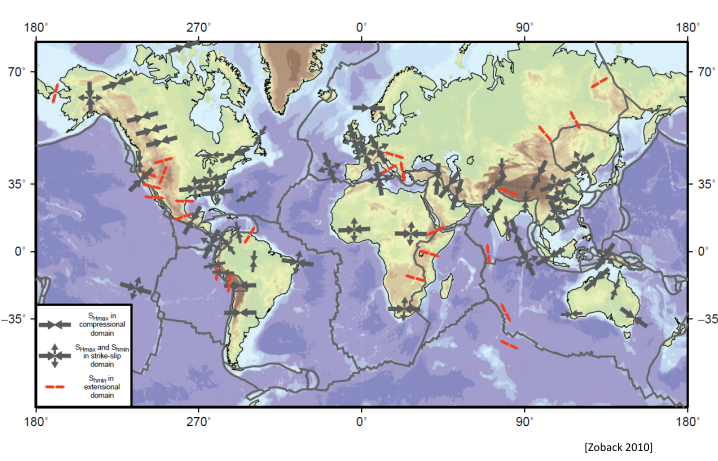
\includegraphics[scale=0.45]{.././Figures/split/1-2.pdf}%
\lthtmlpictureZ
\lthtmlcheckvsize\clearpage}

{\newpage\clearpage
\lthtmlpictureA{tex2html_wrap20875}%
\includegraphics[scale=0.50]{.././Figures/split/1-3.pdf}%
\lthtmlpictureZ
\lthtmlcheckvsize\clearpage}

\stepcounter{section}
\stepcounter{subsection}
{\newpage\clearpage
\lthtmlpictureA{tex2html_wrap20884}%
\includegraphics[scale=0.55]{.././Figures/split/1-4.pdf}%
\lthtmlpictureZ
\lthtmlcheckvsize\clearpage}

\stepcounter{subsection}
{\newpage\clearpage
\lthtmlpictureA{tex2html_wrap20892}%
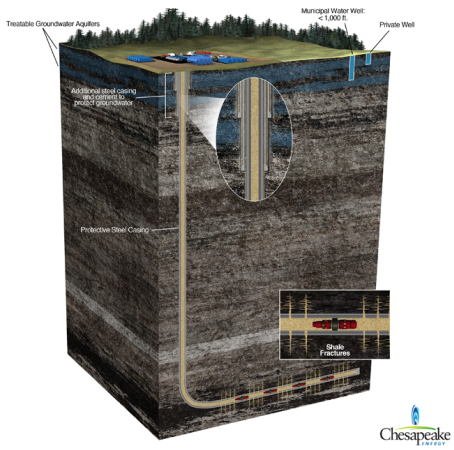
\includegraphics[scale=0.65]{.././Figures/split/1-6.pdf}%
\lthtmlpictureZ
\lthtmlcheckvsize\clearpage}

\stepcounter{subsection}
{\newpage\clearpage
\lthtmlpictureA{tex2html_wrap20898}%
\includegraphics[scale=0.50]{.././Figures/split/1-5.pdf}%
\lthtmlpictureZ
\lthtmlcheckvsize\clearpage}

\stepcounter{section}
\stepcounter{chapter}
\stepcounter{section}
\stepcounter{subsection}
{\newpage\clearpage
\lthtmlinlinemathA{tex2html_wrap_inline20909}%
$ \uline{F}_1$%
\lthtmlindisplaymathZ
\lthtmlcheckvsize\clearpage}

{\newpage\clearpage
\lthtmlinlinemathA{tex2html_wrap_inline20911}%
$ \uline{F}_2$%
\lthtmlindisplaymathZ
\lthtmlcheckvsize\clearpage}

{\newpage\clearpage
\lthtmlinlinemathA{tex2html_wrap_inline20913}%
$ {\rm I\!R}^3$%
\lthtmlindisplaymathZ
\lthtmlcheckvsize\clearpage}

{\newpage\clearpage
\lthtmlinlinemathA{tex2html_wrap_inline20915}%
$ \uline{F}_1 = \uline{F}_2$%
\lthtmlindisplaymathZ
\lthtmlcheckvsize\clearpage}

{\newpage\clearpage
\lthtmlinlinemathA{tex2html_wrap_inline20917}%
$ \uline{F}_1 =  \uline{F}_2 + m \uline{g}$%
\lthtmlindisplaymathZ
\lthtmlcheckvsize\clearpage}

{\newpage\clearpage
\lthtmlinlinemathA{tex2html_wrap_inline20919}%
$ m \uline{g}$%
\lthtmlindisplaymathZ
\lthtmlcheckvsize\clearpage}

{\newpage\clearpage
\lthtmlinlinemathA{tex2html_wrap_inline20921}%
$ \uline{F}$%
\lthtmlindisplaymathZ
\lthtmlcheckvsize\clearpage}

{\newpage\clearpage
\lthtmlinlinemathA{tex2html_wrap_inline20923}%
$ A$%
\lthtmlindisplaymathZ
\lthtmlcheckvsize\clearpage}

{\newpage\clearpage
\lthtmlinlinemathA{tex2html_wrap_indisplay20925}%
$\displaystyle \uline{\sigma} = \frac{\uline{F}}{A}$%
\lthtmlindisplaymathZ
\lthtmlcheckvsize\clearpage}

{\newpage\clearpage
\lthtmlpictureA{tex2html_wrap20927}%
\includegraphics[scale=0.50]{.././Figures/split/2-2.pdf}%
\lthtmlpictureZ
\lthtmlcheckvsize\clearpage}

\stepcounter{subsection}
{\newpage\clearpage
\lthtmlinlinemathA{tex2html_wrap_inline20933}%
$ \Delta x \Delta y \Delta z$%
\lthtmlindisplaymathZ
\lthtmlcheckvsize\clearpage}

{\newpage\clearpage
\lthtmlinlinemathA{tex2html_wrap_inline20935}%
$ \sum \uline{F} = 0$%
\lthtmlindisplaymathZ
\lthtmlcheckvsize\clearpage}

{\newpage\clearpage
\lthtmlinlinemathA{tex2html_wrap_inline20937}%
$ \uline{g}$%
\lthtmlindisplaymathZ
\lthtmlcheckvsize\clearpage}

{\newpage\clearpage
\lthtmlinlinemathA{tex2html_wrap_inline20939}%
$ \sum F_z = 0$%
\lthtmlindisplaymathZ
\lthtmlcheckvsize\clearpage}

{\newpage\clearpage
\lthtmlinlinemathA{tex2html_wrap_indisplay20942}%
$\displaystyle S_v A + \rho_{bulk} Vol  g = S_v A + \Delta S_v A$%
\lthtmlindisplaymathZ
\lthtmlcheckvsize\clearpage}

{\newpage\clearpage
\lthtmlinlinemathA{tex2html_wrap_indisplay20944}%
$\displaystyle \rho_{bulk} \: \Delta x \Delta y \Delta z \:  g = \Delta S_v \Delta x \Delta y$%
\lthtmlindisplaymathZ
\lthtmlcheckvsize\clearpage}

{\newpage\clearpage
\lthtmlinlinemathA{tex2html_wrap_indisplay20946}%
$\displaystyle \frac{\Delta S_v}{\Delta z} = \rho_{bulk} \: g$%
\lthtmlindisplaymathZ
\lthtmlcheckvsize\clearpage}

{\newpage\clearpage
\lthtmlpictureA{tex2html_wrap20948}%
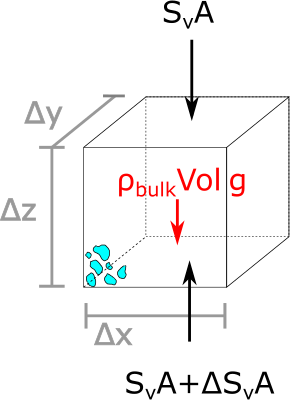
\includegraphics[scale=0.40]{.././Figures/split/2-REVoverburden.pdf}%
\lthtmlpictureZ
\lthtmlcheckvsize\clearpage}

{\newpage\clearpage
\lthtmlinlinemathA{tex2html_wrap_indisplay20953}%
$\displaystyle \int_0^{S_v(z)} dS_v = \int_0^z \rho_{bulk}(z) g \: dz$%
\lthtmlindisplaymathZ
\lthtmlcheckvsize\clearpage}

{\newpage\clearpage
\lthtmlinlinemathA{tex2html_wrap_inline20955}%
$ \rho_{bulk}(z) g$%
\lthtmlindisplaymathZ
\lthtmlcheckvsize\clearpage}

{\newpage\clearpage
\lthtmlinlinemathA{tex2html_wrap_inline20957}%
$ S_v(z=0)=0$%
\lthtmlindisplaymathZ
\lthtmlcheckvsize\clearpage}

{\newpage\clearpage
\lthtmlinlinemathA{tex2html_wrap_inline20959}%
$ \rho_{bulk} = cst$%
\lthtmlindisplaymathZ
\lthtmlcheckvsize\clearpage}

{\newpage\clearpage
\lthtmlinlinemathA{tex2html_wrap_inline20963}%
$ z$%
\lthtmlindisplaymathZ
\lthtmlcheckvsize\clearpage}

{\newpage\clearpage
\lthtmlinlinemathA{tex2html_wrap_indisplay20965}%
$\displaystyle S_v(z)  = \rho_{bulk} g \:z .$%
\lthtmlindisplaymathZ
\lthtmlcheckvsize\clearpage}

{\newpage\clearpage
\lthtmlinlinemathA{tex2html_wrap_inline20967}%
$ \rho_{SiO_2}$%
\lthtmlindisplaymathZ
\lthtmlcheckvsize\clearpage}

{\newpage\clearpage
\lthtmlinlinemathA{tex2html_wrap_inline20969}%
$ \rho_w$%
\lthtmlindisplaymathZ
\lthtmlcheckvsize\clearpage}

{\newpage\clearpage
\lthtmlinlinemathA{tex2html_wrap_inline20971}%
$ \rho_{bulk}$%
\lthtmlindisplaymathZ
\lthtmlcheckvsize\clearpage}

{\newpage\clearpage
\lthtmlinlinemathA{tex2html_wrap_inline20973}%
$ \phi$%
\lthtmlindisplaymathZ
\lthtmlcheckvsize\clearpage}

{\newpage\clearpage
\lthtmlinlinemathA{tex2html_wrap_indisplay20975}%
$\displaystyle \rho_{bulk} = (1-\phi) \rho_{SiO_2} + \phi \rho_w$%
\lthtmlindisplaymathZ
\lthtmlcheckvsize\clearpage}

{\newpage\clearpage
\lthtmlinlinemathA{tex2html_wrap_inline20977}%
$ \rho_{SiO_2} = 2650$%
\lthtmlindisplaymathZ
\lthtmlcheckvsize\clearpage}

{\newpage\clearpage
\lthtmlinlinemathA{tex2html_wrap_inline20979}%
$ ^3$%
\lthtmlindisplaymathZ
\lthtmlcheckvsize\clearpage}

{\newpage\clearpage
\lthtmlinlinemathA{tex2html_wrap_inline20981}%
$ \rho_w = 1000$%
\lthtmlindisplaymathZ
\lthtmlcheckvsize\clearpage}

{\newpage\clearpage
\lthtmlinlinemathA{tex2html_wrap_indisplay20985}%
$\displaystyle \rho_{bulk} = (1-0.2) \times 2650$%
\lthtmlindisplaymathZ
\lthtmlcheckvsize\clearpage}

{\newpage\clearpage
\lthtmlinlinemathA{tex2html_wrap_indisplay20986}%
$\displaystyle ^3 + (0.2) \times 1000$%
\lthtmlindisplaymathZ
\lthtmlcheckvsize\clearpage}

{\newpage\clearpage
\lthtmlinlinemathA{tex2html_wrap_indisplay20987}%
$\displaystyle ^3 = 2320$%
\lthtmlindisplaymathZ
\lthtmlcheckvsize\clearpage}

{\newpage\clearpage
\lthtmlinlinemathA{tex2html_wrap_indisplay20988}%
$\displaystyle ^3 .$%
\lthtmlindisplaymathZ
\lthtmlcheckvsize\clearpage}

{\newpage\clearpage
\lthtmlinlinemathA{tex2html_wrap_indisplay20994}%
$\displaystyle \rho_{bulk} \: g = 2320$%
\lthtmlindisplaymathZ
\lthtmlcheckvsize\clearpage}

{\newpage\clearpage
\lthtmlinlinemathA{tex2html_wrap_indisplay20995}%
$\displaystyle ^3 \times 9.8$%
\lthtmlindisplaymathZ
\lthtmlcheckvsize\clearpage}

{\newpage\clearpage
\lthtmlinlinemathA{tex2html_wrap_indisplay20996}%
$\displaystyle ^2 = 22.7 \times 10^3$%
\lthtmlindisplaymathZ
\lthtmlcheckvsize\clearpage}

{\newpage\clearpage
\lthtmlinlinemathA{tex2html_wrap_indisplay20997}%
$\displaystyle = 22.7$%
\lthtmlindisplaymathZ
\lthtmlcheckvsize\clearpage}

{\newpage\clearpage
\lthtmlinlinemathA{tex2html_wrap_indisplay20998}%
$\displaystyle .$%
\lthtmlindisplaymathZ
\lthtmlcheckvsize\clearpage}

{\newpage\clearpage
\lthtmlinlinemathA{tex2html_wrap_inline21000}%
$ ^2$%
\lthtmlindisplaymathZ
\lthtmlcheckvsize\clearpage}

{\newpage\clearpage
\lthtmlinlinemathA{tex2html_wrap_inline21004}%
$ ^6$%
\lthtmlindisplaymathZ
\lthtmlcheckvsize\clearpage}

{\newpage\clearpage
\lthtmlinlinemathA{tex2html_wrap_inline21008}%
$ g$%
\lthtmlindisplaymathZ
\lthtmlcheckvsize\clearpage}

{\newpage\clearpage
\lthtmlinlinemathA{tex2html_wrap_indisplay21014}%
$\displaystyle \rho_{bulk} g = 144.8$%
\lthtmlindisplaymathZ
\lthtmlcheckvsize\clearpage}

{\newpage\clearpage
\lthtmlinlinemathA{tex2html_wrap_indisplay21015}%
$\displaystyle ^3
= 144.8$%
\lthtmlindisplaymathZ
\lthtmlcheckvsize\clearpage}

{\newpage\clearpage
\lthtmlinlinemathA{tex2html_wrap_indisplay21016}%
$\displaystyle ^2 \times$%
\lthtmlindisplaymathZ
\lthtmlcheckvsize\clearpage}

{\newpage\clearpage
\lthtmlinlinemathA{tex2html_wrap_indisplay21017}%
$\displaystyle = 144.8$%
\lthtmlindisplaymathZ
\lthtmlcheckvsize\clearpage}

{\newpage\clearpage
\lthtmlinlinemathA{tex2html_wrap_indisplay21019}%
$\displaystyle = 1.01$%
\lthtmlindisplaymathZ
\lthtmlcheckvsize\clearpage}

{\newpage\clearpage
\lthtmlinlinemathA{tex2html_wrap_indisplay21020}%
$\displaystyle . \: \: \blacksquare$%
\lthtmlindisplaymathZ
\lthtmlcheckvsize\clearpage}

{\newpage\clearpage
\lthtmlinlinemathA{tex2html_wrap_inline21022}%
$ \sim 1$%
\lthtmlindisplaymathZ
\lthtmlcheckvsize\clearpage}

{\newpage\clearpage
\lthtmlinlinemathA{tex2html_wrap_inline21024}%
$ \sim 23$%
\lthtmlindisplaymathZ
\lthtmlcheckvsize\clearpage}

{\newpage\clearpage
\lthtmlinlinemathA{tex2html_wrap_inline21026}%
$ \phi = 0.20$%
\lthtmlindisplaymathZ
\lthtmlcheckvsize\clearpage}

{\newpage\clearpage
\lthtmlinlinemathA{tex2html_wrap_inline21028}%
$ \sim 0.44$%
\lthtmlindisplaymathZ
\lthtmlcheckvsize\clearpage}

{\newpage\clearpage
\lthtmlinlinemathA{tex2html_wrap_inline21030}%
$ \sim 10$%
\lthtmlindisplaymathZ
\lthtmlcheckvsize\clearpage}

{\newpage\clearpage
\lthtmlinlinemathA{tex2html_wrap_inline21032}%
$ S_w, S_o, S_g$%
\lthtmlindisplaymathZ
\lthtmlcheckvsize\clearpage}

\stepcounter{subsubsection}
{\newpage\clearpage
\lthtmlinlinemathA{tex2html_wrap_indisplay21041}%
$\displaystyle P_p = \rho_w g \, z$%
\lthtmlindisplaymathZ
\lthtmlcheckvsize\clearpage}

{\newpage\clearpage
\lthtmlpictureA{tex2html_wrap21053}%
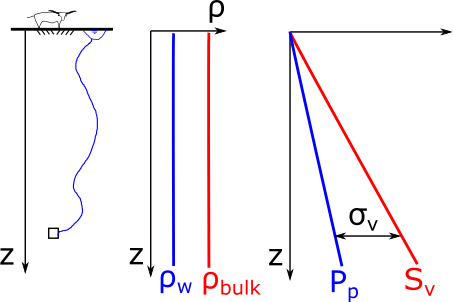
\includegraphics[scale=0.55]{.././Figures/split/2-OnshorePpSv.pdf}%
\lthtmlpictureZ
\lthtmlcheckvsize\clearpage}

{\newpage\clearpage
\lthtmlinlinemathA{tex2html_wrap_indisplay21070}%
$\displaystyle \sigma_v = S_v - P_p$%
\lthtmlindisplaymathZ
\lthtmlcheckvsize\clearpage}

{\newpage\clearpage
\lthtmlinlinemathA{tex2html_wrap_inline21072}%
$ S_v > P_p$%
\lthtmlindisplaymathZ
\lthtmlcheckvsize\clearpage}

{\newpage\clearpage
\lthtmlpictureA{tex2html_wrap21074}%
\includegraphics[scale=0.55]{.././Figures/split/2-20.pdf}%
\lthtmlpictureZ
\lthtmlcheckvsize\clearpage}

{\newpage\clearpage
\lthtmlinlinemathA{tex2html_wrap_inline21079}%
$ P_w$%
\lthtmlindisplaymathZ
\lthtmlcheckvsize\clearpage}

{\newpage\clearpage
\lthtmlinlinemathA{tex2html_wrap_indisplay21095}%
$\displaystyle \frac{dP_p}{dz} = \rho_w g = 1040$%
\lthtmlindisplaymathZ
\lthtmlcheckvsize\clearpage}

{\newpage\clearpage
\lthtmlinlinemathA{tex2html_wrap_indisplay21097}%
$\displaystyle ^2 = 10.19$%
\lthtmlindisplaymathZ
\lthtmlcheckvsize\clearpage}

{\newpage\clearpage
\lthtmlinlinemathA{tex2html_wrap_indisplay21099}%
$\displaystyle \frac{dS_v}{dz} = \rho_{bulk} g = 2350$%
\lthtmlindisplaymathZ
\lthtmlcheckvsize\clearpage}

{\newpage\clearpage
\lthtmlinlinemathA{tex2html_wrap_indisplay21101}%
$\displaystyle ^2 = 23.03$%
\lthtmlindisplaymathZ
\lthtmlcheckvsize\clearpage}

{\newpage\clearpage
\lthtmlinlinemathA{tex2html_wrap_indisplay21103}%
$\displaystyle P_p = \frac{dP_p}{dz} z = 10.19$%
\lthtmlindisplaymathZ
\lthtmlcheckvsize\clearpage}

{\newpage\clearpage
\lthtmlinlinemathA{tex2html_wrap_indisplay21104}%
$\displaystyle \times 1.219$%
\lthtmlindisplaymathZ
\lthtmlcheckvsize\clearpage}

{\newpage\clearpage
\lthtmlinlinemathA{tex2html_wrap_indisplay21105}%
$\displaystyle =  12.43$%
\lthtmlindisplaymathZ
\lthtmlcheckvsize\clearpage}

{\newpage\clearpage
\lthtmlinlinemathA{tex2html_wrap_indisplay21106}%
$\displaystyle = 1801$%
\lthtmlindisplaymathZ
\lthtmlcheckvsize\clearpage}

{\newpage\clearpage
\lthtmlinlinemathA{tex2html_wrap_indisplay21108}%
$\displaystyle \frac{dS_v}{dz} z = 23.03$%
\lthtmlindisplaymathZ
\lthtmlcheckvsize\clearpage}

{\newpage\clearpage
\lthtmlinlinemathA{tex2html_wrap_indisplay21110}%
$\displaystyle =  28.07$%
\lthtmlindisplaymathZ
\lthtmlcheckvsize\clearpage}

{\newpage\clearpage
\lthtmlinlinemathA{tex2html_wrap_indisplay21111}%
$\displaystyle = 4070$%
\lthtmlindisplaymathZ
\lthtmlcheckvsize\clearpage}

{\newpage\clearpage
\lthtmlinlinemathA{tex2html_wrap_inline21114}%
$ \: \: \blacksquare$%
\lthtmlindisplaymathZ
\lthtmlcheckvsize\clearpage}

\stepcounter{subsubsection}
{\newpage\clearpage
\lthtmlinlinemathA{tex2html_wrap_inline21117}%
$ z_w$%
\lthtmlindisplaymathZ
\lthtmlcheckvsize\clearpage}

{\newpage\clearpage
\lthtmlinlinemathA{tex2html_wrap_inline21121}%
$ z > z_w$%
\lthtmlindisplaymathZ
\lthtmlcheckvsize\clearpage}

{\newpage\clearpage
\lthtmlinlinemathA{tex2html_wrap_indisplay21123}%
$\displaystyle S_v = \rho_{w} g \, z_w + \rho_{bulk} g (z-z_w)$%
\lthtmlindisplaymathZ
\lthtmlcheckvsize\clearpage}

{\newpage\clearpage
\lthtmlinlinemathA{tex2html_wrap_indisplay21124}%
$\displaystyle \quad z \geq z_w$%
\lthtmlindisplaymathZ
\lthtmlcheckvsize\clearpage}

{\newpage\clearpage
\lthtmlpictureA{tex2html_wrap21126}%
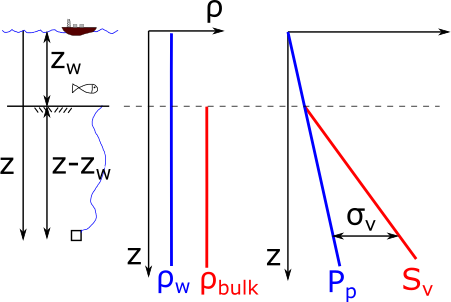
\includegraphics[scale=0.55]{.././Figures/split/2-OffshorePpSv.pdf}%
\lthtmlpictureZ
\lthtmlcheckvsize\clearpage}

{\newpage\clearpage
\lthtmlinlinemathA{tex2html_wrap_inline21131}%
$ z=z_w$%
\lthtmlindisplaymathZ
\lthtmlcheckvsize\clearpage}

{\newpage\clearpage
\lthtmlinlinemathA{tex2html_wrap_indisplay21133}%
$\displaystyle \sigma_v = S_v - P_p =  \rho_{bulk} g (z-z_w)$%
\lthtmlindisplaymathZ
\lthtmlcheckvsize\clearpage}

{\newpage\clearpage
\lthtmlinlinemathA{tex2html_wrap_indisplay21140}%
$\displaystyle P_p = \rho_w g z_w + \frac{dP_p}{dz} (z-z_w)  = 0.44$%
\lthtmlindisplaymathZ
\lthtmlcheckvsize\clearpage}

{\newpage\clearpage
\lthtmlinlinemathA{tex2html_wrap_indisplay21141}%
$\displaystyle \times 2000$%
\lthtmlindisplaymathZ
\lthtmlcheckvsize\clearpage}

{\newpage\clearpage
\lthtmlinlinemathA{tex2html_wrap_indisplay21142}%
$\displaystyle + 0.44$%
\lthtmlindisplaymathZ
\lthtmlcheckvsize\clearpage}

{\newpage\clearpage
\lthtmlinlinemathA{tex2html_wrap_indisplay21143}%
$\displaystyle \times (9000-2000)$%
\lthtmlindisplaymathZ
\lthtmlcheckvsize\clearpage}

{\newpage\clearpage
\lthtmlinlinemathA{tex2html_wrap_indisplay21144}%
$\displaystyle =   3960$%
\lthtmlindisplaymathZ
\lthtmlcheckvsize\clearpage}

{\newpage\clearpage
\lthtmlinlinemathA{tex2html_wrap_indisplay21146}%
$\displaystyle S_v = \rho_w g z_w + \frac{dS_v}{dz} (z-z_w)  = 0.44$%
\lthtmlindisplaymathZ
\lthtmlcheckvsize\clearpage}

{\newpage\clearpage
\lthtmlinlinemathA{tex2html_wrap_indisplay21148}%
$\displaystyle + 1.00$%
\lthtmlindisplaymathZ
\lthtmlcheckvsize\clearpage}

{\newpage\clearpage
\lthtmlinlinemathA{tex2html_wrap_indisplay21150}%
$\displaystyle = 7880$%
\lthtmlindisplaymathZ
\lthtmlcheckvsize\clearpage}

{\newpage\clearpage
\lthtmlinlinemathA{tex2html_wrap_indisplay21151}%
$\displaystyle ,$%
\lthtmlindisplaymathZ
\lthtmlcheckvsize\clearpage}

{\newpage\clearpage
\lthtmlinlinemathA{tex2html_wrap_indisplay21153}%
$\displaystyle \sigma_v = S_v - P_p = 7880$%
\lthtmlindisplaymathZ
\lthtmlcheckvsize\clearpage}

{\newpage\clearpage
\lthtmlinlinemathA{tex2html_wrap_indisplay21154}%
$\displaystyle - 3960$%
\lthtmlindisplaymathZ
\lthtmlcheckvsize\clearpage}

{\newpage\clearpage
\lthtmlinlinemathA{tex2html_wrap_indisplay21155}%
$\displaystyle = 3920$%
\lthtmlindisplaymathZ
\lthtmlcheckvsize\clearpage}

{\newpage\clearpage
\lthtmlinlinemathA{tex2html_wrap_inline21158}%
$ P_p = 27.31$%
\lthtmlindisplaymathZ
\lthtmlcheckvsize\clearpage}

{\newpage\clearpage
\lthtmlinlinemathA{tex2html_wrap_inline21160}%
$ S_v =  54.34$%
\lthtmlindisplaymathZ
\lthtmlcheckvsize\clearpage}

{\newpage\clearpage
\lthtmlinlinemathA{tex2html_wrap_inline21162}%
$ \sigma_v = 27.03$%
\lthtmlindisplaymathZ
\lthtmlcheckvsize\clearpage}

\stepcounter{subsubsection}
{\newpage\clearpage
\lthtmlinlinemathA{tex2html_wrap_indisplay21169}%
$\displaystyle S_v(z) = \int_0^z \rho_{bulk}(z) g \: dz$%
\lthtmlindisplaymathZ
\lthtmlcheckvsize\clearpage}

{\newpage\clearpage
\lthtmlinlinemathA{tex2html_wrap_inline21171}%
$ \rho_{bulk}(z)$%
\lthtmlindisplaymathZ
\lthtmlcheckvsize\clearpage}

{\newpage\clearpage
\lthtmlinlinemathA{tex2html_wrap_indisplay21179}%
$\displaystyle S_v(z_i) = \sum\limits_1^i \rho_{bulk}(z_i) g \Delta z_i$%
\lthtmlindisplaymathZ
\lthtmlcheckvsize\clearpage}

{\newpage\clearpage
\lthtmlinlinemathA{tex2html_wrap_inline21181}%
$ i$%
\lthtmlindisplaymathZ
\lthtmlcheckvsize\clearpage}

{\newpage\clearpage
\lthtmlinlinemathA{tex2html_wrap_inline21183}%
$ z_i$%
\lthtmlindisplaymathZ
\lthtmlcheckvsize\clearpage}

{\newpage\clearpage
\lthtmlpictureA{tex2html_wrap21187}%
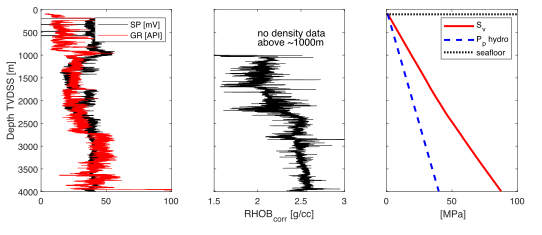
\includegraphics[scale=0.85]{.././Figures/split/2-VertStress_TVDSS.pdf}%
\lthtmlpictureZ
\lthtmlcheckvsize\clearpage}

\stepcounter{section}
{\newpage\clearpage
\lthtmlinlinemathA{tex2html_wrap_inline21193}%
$ z \sim 8,500$%
\lthtmlindisplaymathZ
\lthtmlcheckvsize\clearpage}

{\newpage\clearpage
\lthtmlinlinemathA{tex2html_wrap_inline21197}%
$ z \sim 11,000$%
\lthtmlindisplaymathZ
\lthtmlcheckvsize\clearpage}

{\newpage\clearpage
\lthtmlpictureA{tex2html_wrap21201}%
\includegraphics[scale=0.65]{.././Figures/split/2-9.pdf}%
\lthtmlpictureZ
\lthtmlcheckvsize\clearpage}

{\newpage\clearpage
\lthtmlinlinemathA{tex2html_wrap_inline21206}%
$ \lambda_p$%
\lthtmlindisplaymathZ
\lthtmlcheckvsize\clearpage}

{\newpage\clearpage
\lthtmlinlinemathA{tex2html_wrap_indisplay21208}%
$\displaystyle \lambda_p(z) = \frac{P_p(z)}{S_v(z)}$%
\lthtmlindisplaymathZ
\lthtmlcheckvsize\clearpage}

{\newpage\clearpage
\lthtmlinlinemathA{tex2html_wrap_inline21214}%
$ \lambda_p \leq 1$%
\lthtmlindisplaymathZ
\lthtmlcheckvsize\clearpage}

{\newpage\clearpage
\lthtmlinlinemathA{tex2html_wrap_inline21216}%
$ \lambda_p \sim 0.44$%
\lthtmlindisplaymathZ
\lthtmlcheckvsize\clearpage}

{\newpage\clearpage
\lthtmlinlinemathA{tex2html_wrap_inline21218}%
$ \lambda_p \neq 0.44$%
\lthtmlindisplaymathZ
\lthtmlcheckvsize\clearpage}

{\newpage\clearpage
\lthtmlinlinemathA{tex2html_wrap_inline21220}%
$ \lambda_p \rightarrow 1$%
\lthtmlindisplaymathZ
\lthtmlcheckvsize\clearpage}

\stepcounter{subsection}
{\newpage\clearpage
\lthtmlinlinemathA{tex2html_wrap_inline21223}%
$ P_p > P_p^{\text{hydrostatic}}$%
\lthtmlindisplaymathZ
\lthtmlcheckvsize\clearpage}

{\newpage\clearpage
\lthtmlinlinemathA{tex2html_wrap_inline21225}%
$ \Delta P_p$%
\lthtmlindisplaymathZ
\lthtmlcheckvsize\clearpage}

{\newpage\clearpage
\lthtmlinlinemathA{tex2html_wrap_inline21227}%
$ h$%
\lthtmlindisplaymathZ
\lthtmlcheckvsize\clearpage}

{\newpage\clearpage
\lthtmlinlinemathA{tex2html_wrap_inline21229}%
$ \rho_{brine} - \rho_{hydrocarbon}$%
\lthtmlindisplaymathZ
\lthtmlcheckvsize\clearpage}

{\newpage\clearpage
\lthtmlinlinemathA{tex2html_wrap_indisplay21231}%
$\displaystyle \Delta P = (\rho_{brine} - \rho_{hydrocarbon}) g  h$%
\lthtmlindisplaymathZ
\lthtmlcheckvsize\clearpage}

{\newpage\clearpage
\lthtmlpictureA{tex2html_wrap21239}%
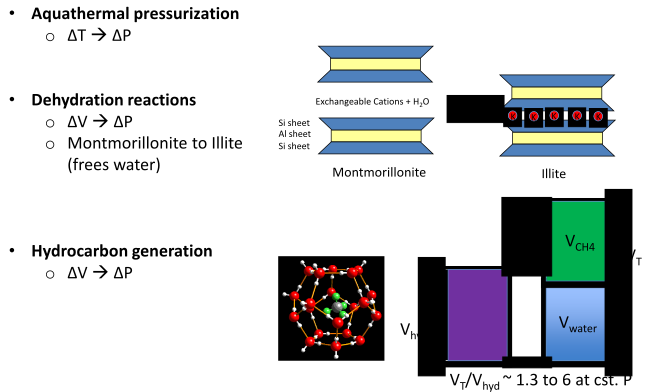
\includegraphics[scale=0.50]{.././Figures/split/2-11.pdf}%
\lthtmlpictureZ
\lthtmlcheckvsize\clearpage}

\stepcounter{subsection}
{\newpage\clearpage
\lthtmlinlinemathA{tex2html_wrap_inline21245}%
$ W$%
\lthtmlindisplaymathZ
\lthtmlcheckvsize\clearpage}

{\newpage\clearpage
\lthtmlinlinemathA{tex2html_wrap_inline21247}%
$ \Delta P = W/A$%
\lthtmlindisplaymathZ
\lthtmlcheckvsize\clearpage}

{\newpage\clearpage
\lthtmlinlinemathA{tex2html_wrap_inline21255}%
$ \sigma_v = W/A$%
\lthtmlindisplaymathZ
\lthtmlcheckvsize\clearpage}

{\newpage\clearpage
\lthtmlinlinemathA{tex2html_wrap_inline21259}%
$ \Delta P = 0$%
\lthtmlindisplaymathZ
\lthtmlcheckvsize\clearpage}

{\newpage\clearpage
\lthtmlpictureA{tex2html_wrap21263}%
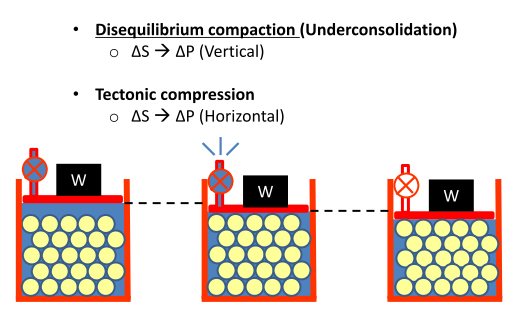
\includegraphics[scale=0.50]{.././Figures/split/2-12.pdf}%
\lthtmlpictureZ
\lthtmlcheckvsize\clearpage}

{\newpage\clearpage
\lthtmlpictureA{tex2html_wrap21268}%
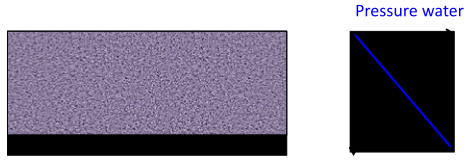
\includegraphics[scale=0.60]{.././Figures/split/2-13.pdf}%
\lthtmlpictureZ
\lthtmlcheckvsize\clearpage}

{\newpage\clearpage
\lthtmlinlinemathA{tex2html_wrap_inline21273}%
$ \Delta z$%
\lthtmlindisplaymathZ
\lthtmlcheckvsize\clearpage}

{\newpage\clearpage
\lthtmlinlinemathA{tex2html_wrap_indisplay21275}%
$\displaystyle D_h = \frac{M k} {\mu}$%
\lthtmlindisplaymathZ
\lthtmlcheckvsize\clearpage}

{\newpage\clearpage
\lthtmlinlinemathA{tex2html_wrap_inline21279}%
$ C_{bp}$%
\lthtmlindisplaymathZ
\lthtmlcheckvsize\clearpage}

{\newpage\clearpage
\lthtmlinlinemathA{tex2html_wrap_inline21281}%
$ k$%
\lthtmlindisplaymathZ
\lthtmlcheckvsize\clearpage}

{\newpage\clearpage
\lthtmlinlinemathA{tex2html_wrap_inline21283}%
$ \mu$%
\lthtmlindisplaymathZ
\lthtmlcheckvsize\clearpage}

{\newpage\clearpage
\lthtmlinlinemathA{tex2html_wrap_indisplay21285}%
$\displaystyle \frac{\partial P_p}{\partial t} = D_h \frac{d^2P_p}{dz^2}$%
\lthtmlindisplaymathZ
\lthtmlcheckvsize\clearpage}

{\newpage\clearpage
\lthtmlpictureA{tex2html_wrap21287}%
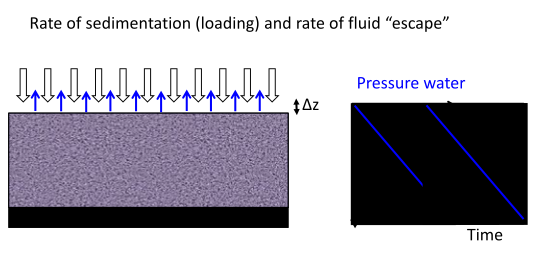
\includegraphics[scale=0.60]{.././Figures/split/2-14.pdf}%
\lthtmlpictureZ
\lthtmlcheckvsize\clearpage}

{\newpage\clearpage
\lthtmlinlinemathA{tex2html_wrap_inline21292}%
$ T_{ch}$%
\lthtmlindisplaymathZ
\lthtmlcheckvsize\clearpage}

{\newpage\clearpage
\lthtmlinlinemathA{tex2html_wrap_inline21294}%
$ \sim 2/3$%
\lthtmlindisplaymathZ
\lthtmlcheckvsize\clearpage}

{\newpage\clearpage
\lthtmlinlinemathA{tex2html_wrap_indisplay21296}%
$\displaystyle T_{ch} = \frac{L^2}{D_h}$%
\lthtmlindisplaymathZ
\lthtmlcheckvsize\clearpage}

{\newpage\clearpage
\lthtmlinlinemathA{tex2html_wrap_inline21298}%
$ L$%
\lthtmlindisplaymathZ
\lthtmlcheckvsize\clearpage}

{\newpage\clearpage
\lthtmlinlinemathA{tex2html_wrap_inline21302}%
$ k =$%
\lthtmlindisplaymathZ
\lthtmlcheckvsize\clearpage}

{\newpage\clearpage
\lthtmlinlinemathA{tex2html_wrap_inline21304}%
$ M =$%
\lthtmlindisplaymathZ
\lthtmlcheckvsize\clearpage}

{\newpage\clearpage
\lthtmlinlinemathA{tex2html_wrap_inline21310}%
$ T_{ch} \sim $%
\lthtmlindisplaymathZ
\lthtmlcheckvsize\clearpage}

{\newpage\clearpage
\lthtmlinlinemathA{tex2html_wrap_indisplay21318}%
$\displaystyle \phi = \phi_o \exp (-\beta \sigma_v)$%
\lthtmlindisplaymathZ
\lthtmlcheckvsize\clearpage}

{\newpage\clearpage
\lthtmlpictureA{tex2html_wrap21324}%
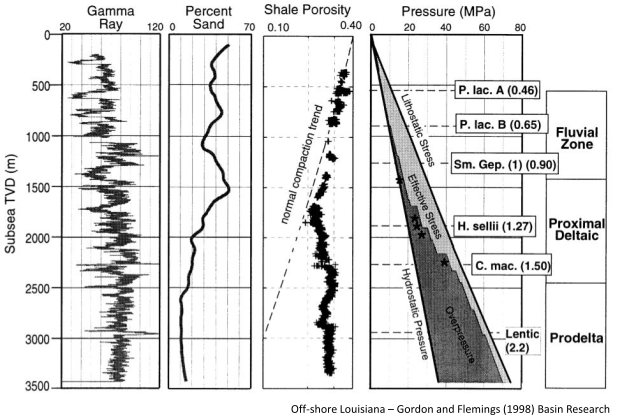
\includegraphics[scale=0.65]{.././Figures/split/2-16.pdf}%
\lthtmlpictureZ
\lthtmlcheckvsize\clearpage}

{\newpage\clearpage
\lthtmlinlinemathA{tex2html_wrap_inline21337}%
$ \phi = 0.298$%
\lthtmlindisplaymathZ
\lthtmlcheckvsize\clearpage}

{\newpage\clearpage
\lthtmlinlinemathA{tex2html_wrap_inline21339}%
$ \beta = 3.2 \times 10^{-2}$%
\lthtmlindisplaymathZ
\lthtmlcheckvsize\clearpage}

{\newpage\clearpage
\lthtmlinlinemathA{tex2html_wrap_inline21341}%
$ ^{-1}$%
\lthtmlindisplaymathZ
\lthtmlcheckvsize\clearpage}

{\newpage\clearpage
\lthtmlinlinemathA{tex2html_wrap_inline21343}%
$ \phi_0 = 0.38$%
\lthtmlindisplaymathZ
\lthtmlcheckvsize\clearpage}

{\newpage\clearpage
\lthtmlinlinemathA{tex2html_wrap_indisplay21345}%
$\displaystyle S_v = 10$%
\lthtmlindisplaymathZ
\lthtmlcheckvsize\clearpage}

{\newpage\clearpage
\lthtmlinlinemathA{tex2html_wrap_indisplay21346}%
$\displaystyle \times 0.5$%
\lthtmlindisplaymathZ
\lthtmlcheckvsize\clearpage}

{\newpage\clearpage
\lthtmlinlinemathA{tex2html_wrap_indisplay21347}%
$\displaystyle + 22$%
\lthtmlindisplaymathZ
\lthtmlcheckvsize\clearpage}

{\newpage\clearpage
\lthtmlinlinemathA{tex2html_wrap_indisplay21348}%
$\displaystyle \times 1.5$%
\lthtmlindisplaymathZ
\lthtmlcheckvsize\clearpage}

{\newpage\clearpage
\lthtmlinlinemathA{tex2html_wrap_indisplay21349}%
$\displaystyle = 38$%
\lthtmlindisplaymathZ
\lthtmlcheckvsize\clearpage}

{\newpage\clearpage
\lthtmlinlinemathA{tex2html_wrap_indisplay21352}%
$\displaystyle \sigma_v = - \frac{\ln \left( \phi / \phi_o \right)}{\beta} = 7.6$%
\lthtmlindisplaymathZ
\lthtmlcheckvsize\clearpage}

{\newpage\clearpage
\lthtmlinlinemathA{tex2html_wrap_inline21355}%
$ S_v = \sigma_v + P_p$%
\lthtmlindisplaymathZ
\lthtmlcheckvsize\clearpage}

{\newpage\clearpage
\lthtmlinlinemathA{tex2html_wrap_indisplay21357}%
$\displaystyle P_p = S_v - \sigma_v =
38$%
\lthtmlindisplaymathZ
\lthtmlcheckvsize\clearpage}

{\newpage\clearpage
\lthtmlinlinemathA{tex2html_wrap_indisplay21358}%
$\displaystyle - 7.6$%
\lthtmlindisplaymathZ
\lthtmlcheckvsize\clearpage}

{\newpage\clearpage
\lthtmlinlinemathA{tex2html_wrap_indisplay21359}%
$\displaystyle = 30.40$%
\lthtmlindisplaymathZ
\lthtmlcheckvsize\clearpage}

{\newpage\clearpage
\lthtmlinlinemathA{tex2html_wrap_indisplay21362}%
$\displaystyle \lambda_p = \frac{P_p}{S_v} = 	\frac{30.40 \text{ MPa}}{38 \text{ MPa}} = 0.8. \: \: \blacksquare$%
\lthtmlindisplaymathZ
\lthtmlcheckvsize\clearpage}

\stepcounter{subsection}
{\newpage\clearpage
\lthtmlpictureA{tex2html_wrap21365}%
\includegraphics[scale=0.65]{.././Figures/split/2-17.pdf}%
\lthtmlpictureZ
\lthtmlcheckvsize\clearpage}

\stepcounter{section}
\stepcounter{subsection}
{\newpage\clearpage
\lthtmlinlinemathA{tex2html_wrap_inline21378}%
$ S_{Hmax} \geq S_{hmin}$%
\lthtmlindisplaymathZ
\lthtmlcheckvsize\clearpage}

{\newpage\clearpage
\lthtmlpictureA{tex2html_wrap21380}%
\includegraphics[scale=0.50]{.././Figures/split/3-20.pdf}%
\lthtmlpictureZ
\lthtmlcheckvsize\clearpage}

{\newpage\clearpage
\lthtmlpictureA{tex2html_wrap21385}%
\includegraphics[scale=0.50]{.././Figures/split/3-16.pdf}%
\lthtmlpictureZ
\lthtmlcheckvsize\clearpage}

{\newpage\clearpage
\lthtmlpictureA{tex2html_wrap21390}%
\includegraphics[scale=0.55]{.././Figures/split/3-18.pdf}%
\lthtmlpictureZ
\lthtmlcheckvsize\clearpage}

\stepcounter{subsection}
{\newpage\clearpage
\lthtmlpictureA{tex2html_wrap21398}%
\includegraphics[scale=0.55]{.././Figures/split/3-2.pdf}%
\lthtmlpictureZ
\lthtmlcheckvsize\clearpage}

\stepcounter{subsection}
{\newpage\clearpage
\lthtmlinlinemathA{tex2html_wrap_inline21406}%
$ S_v > S_{hmin} = S_3$%
\lthtmlindisplaymathZ
\lthtmlcheckvsize\clearpage}

\stepcounter{subsection}
{\newpage\clearpage
\lthtmlinlinemathA{tex2html_wrap_inline21433}%
$ S_2$%
\lthtmlindisplaymathZ
\lthtmlcheckvsize\clearpage}

\stepcounter{subsubsection}
{\newpage\clearpage
\lthtmlinlinemathA{tex2html_wrap_inline21499}%
$ S_v > S_{Hmax} > S_{hmin}$%
\lthtmlindisplaymathZ
\lthtmlcheckvsize\clearpage}

{\newpage\clearpage
\lthtmlinlinemathA{tex2html_wrap_inline21501}%
$ S_1 = S_v$%
\lthtmlindisplaymathZ
\lthtmlcheckvsize\clearpage}

{\newpage\clearpage
\lthtmlinlinemathA{tex2html_wrap_inline21503}%
$ S_2 = S_{Hmax}$%
\lthtmlindisplaymathZ
\lthtmlcheckvsize\clearpage}

{\newpage\clearpage
\lthtmlinlinemathA{tex2html_wrap_inline21505}%
$ S_3 = S_{hmin}$%
\lthtmlindisplaymathZ
\lthtmlcheckvsize\clearpage}

{\newpage\clearpage
\lthtmlinlinemathA{tex2html_wrap_inline21509}%
$ \sim 60$%
\lthtmlindisplaymathZ
\lthtmlcheckvsize\clearpage}

{\newpage\clearpage
\lthtmlinlinemathA{tex2html_wrap_inline21513}%
$ \sigma_1 = S_1 - P_p$%
\lthtmlindisplaymathZ
\lthtmlcheckvsize\clearpage}

{\newpage\clearpage
\lthtmlinlinemathA{tex2html_wrap_inline21515}%
$ \sigma_3 = S_3 - P_p$%
\lthtmlindisplaymathZ
\lthtmlcheckvsize\clearpage}

{\newpage\clearpage
\lthtmlpictureA{tex2html_wrap21519}%
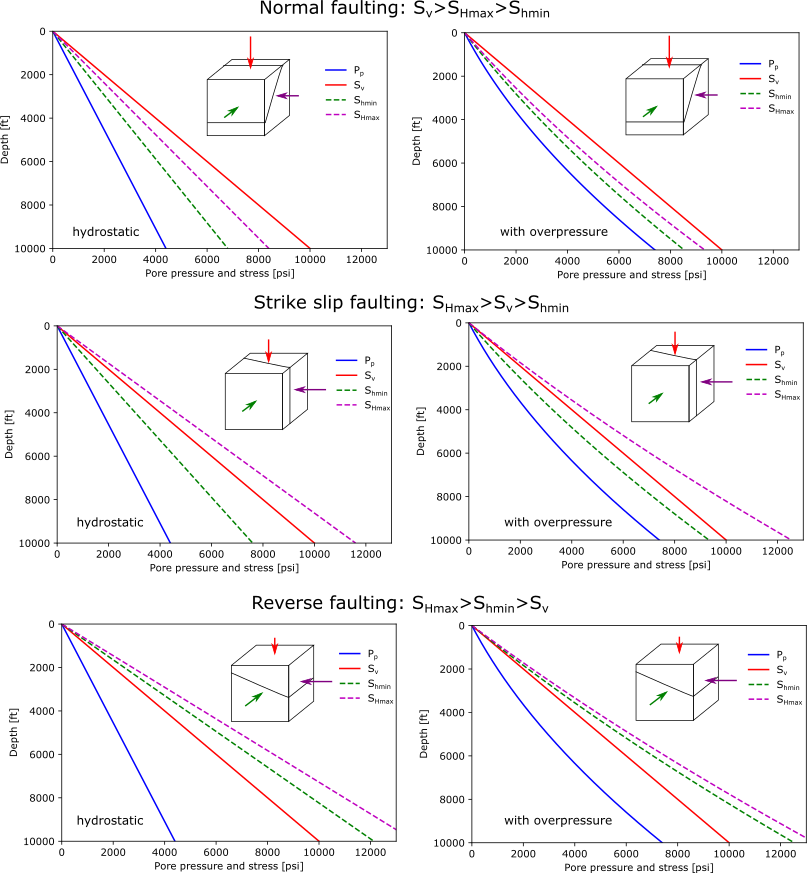
\includegraphics[scale=0.55]{.././Figures/split/2-StressProfiles.pdf}%
\lthtmlpictureZ
\lthtmlcheckvsize\clearpage}

\stepcounter{subsubsection}
{\newpage\clearpage
\lthtmlinlinemathA{tex2html_wrap_inline21525}%
$ S_{Hmax} > S_v > S_{hmin}$%
\lthtmlindisplaymathZ
\lthtmlcheckvsize\clearpage}

{\newpage\clearpage
\lthtmlinlinemathA{tex2html_wrap_inline21527}%
$ S_1 = S_{Hmax}$%
\lthtmlindisplaymathZ
\lthtmlcheckvsize\clearpage}

{\newpage\clearpage
\lthtmlinlinemathA{tex2html_wrap_inline21529}%
$ S_2 = S_v$%
\lthtmlindisplaymathZ
\lthtmlcheckvsize\clearpage}

\stepcounter{subsubsection}
{\newpage\clearpage
\lthtmlinlinemathA{tex2html_wrap_inline21540}%
$ S_{Hmax} > S_{hmin} > S_v$%
\lthtmlindisplaymathZ
\lthtmlcheckvsize\clearpage}

{\newpage\clearpage
\lthtmlinlinemathA{tex2html_wrap_inline21544}%
$ S_2 = S_{hmin}$%
\lthtmlindisplaymathZ
\lthtmlcheckvsize\clearpage}

{\newpage\clearpage
\lthtmlinlinemathA{tex2html_wrap_inline21546}%
$ S_3 = S_v$%
\lthtmlindisplaymathZ
\lthtmlcheckvsize\clearpage}

\stepcounter{subsection}
{\newpage\clearpage
\lthtmlinlinemathA{tex2html_wrap_inline21555}%
$ \rho_w g z$%
\lthtmlindisplaymathZ
\lthtmlcheckvsize\clearpage}

{\newpage\clearpage
\lthtmlinlinemathA{tex2html_wrap_inline21571}%
$ S_3 = S_{22}$%
\lthtmlindisplaymathZ
\lthtmlcheckvsize\clearpage}

{\newpage\clearpage
\lthtmlinlinemathA{tex2html_wrap_inline21573}%
$ S_3 = S_{11}$%
\lthtmlindisplaymathZ
\lthtmlcheckvsize\clearpage}

{\newpage\clearpage
\lthtmlinlinemathA{tex2html_wrap_inline21575}%
$ S_3 = S_{33}$%
\lthtmlindisplaymathZ
\lthtmlcheckvsize\clearpage}

{\newpage\clearpage
\lthtmlinlinemathA{tex2html_wrap_inline21577}%
$ S_{hmin} < S_{Hmax} < S_v$%
\lthtmlindisplaymathZ
\lthtmlcheckvsize\clearpage}

\stepcounter{section}
{\newpage\clearpage
\lthtmlinlinemathA{tex2html_wrap_inline21618}%
$ \beta = 3 \times 10^{-2}$%
\lthtmlindisplaymathZ
\lthtmlcheckvsize\clearpage}

{\newpage\clearpage
\lthtmlinlinemathA{tex2html_wrap_inline21624}%
$ [$%
\lthtmlindisplaymathZ
\lthtmlcheckvsize\clearpage}

{\newpage\clearpage
\lthtmlinlinemathA{tex2html_wrap_inline21626}%
$ ]$%
\lthtmlindisplaymathZ
\lthtmlcheckvsize\clearpage}

{\newpage\clearpage
\lthtmlinlinemathA{tex2html_wrap_inline21630}%
$ ^3]$%
\lthtmlindisplaymathZ
\lthtmlcheckvsize\clearpage}

{\newpage\clearpage
\lthtmlinlinemathA{tex2html_wrap_inline21632}%
$ [-]$%
\lthtmlindisplaymathZ
\lthtmlcheckvsize\clearpage}

\stepcounter{section}
\stepcounter{chapter}
\stepcounter{section}
{\newpage\clearpage
\lthtmlinlinemathA{tex2html_wrap_inline21733}%
$ \uline{e}_1$%
\lthtmlindisplaymathZ
\lthtmlcheckvsize\clearpage}

{\newpage\clearpage
\lthtmlinlinemathA{tex2html_wrap_inline21735}%
$ \uline{e}_2$%
\lthtmlindisplaymathZ
\lthtmlcheckvsize\clearpage}

{\newpage\clearpage
\lthtmlinlinemathA{tex2html_wrap_inline21737}%
$ \uline{e}_3$%
\lthtmlindisplaymathZ
\lthtmlcheckvsize\clearpage}

{\newpage\clearpage
\lthtmlinlinemathA{tex2html_wrap_inline21745}%
$ T$%
\lthtmlindisplaymathZ
\lthtmlcheckvsize\clearpage}

{\newpage\clearpage
\lthtmlinlinemathA{tex2html_wrap_inline21751}%
$ \uline{v}$%
\lthtmlindisplaymathZ
\lthtmlcheckvsize\clearpage}

{\newpage\clearpage
\lthtmlinlinemathA{tex2html_wrap_inline21775}%
$ S_{ij}=S_{ji}$%
\lthtmlindisplaymathZ
\lthtmlcheckvsize\clearpage}

{\newpage\clearpage
\lthtmlinlinemathA{tex2html_wrap_inline21777}%
$ i \neq j$%
\lthtmlindisplaymathZ
\lthtmlcheckvsize\clearpage}

{\newpage\clearpage
\lthtmlpictureA{tex2html_wrap21779}%
\includegraphics[scale=0.55]{.././Figures/split/4-3.pdf}%
\lthtmlpictureZ
\lthtmlcheckvsize\clearpage}

{\newpage\clearpage
\lthtmlinlinemathA{tex2html_wrap_inline21812}%
$ S_1 \geq S_2 \geq S_3$%
\lthtmlindisplaymathZ
\lthtmlcheckvsize\clearpage}

{\newpage\clearpage
\lthtmlpictureA{tex2html_wrap21816}%
\includegraphics[scale=0.55]{.././Figures/split/4-4.pdf}%
\lthtmlpictureZ
\lthtmlcheckvsize\clearpage}

\stepcounter{subsection}
{\newpage\clearpage
\lthtmlinlinemathA{tex2html_wrap_inline21822}%
$ \uline{a}$%
\lthtmlindisplaymathZ
\lthtmlcheckvsize\clearpage}

{\newpage\clearpage
\lthtmlinlinemathA{tex2html_wrap_inline21824}%
$ m \uline{a} = 0$%
\lthtmlindisplaymathZ
\lthtmlcheckvsize\clearpage}

{\newpage\clearpage
\lthtmlinlinemathA{tex2html_wrap_inline21826}%
$ \rho V b_1$%
\lthtmlindisplaymathZ
\lthtmlcheckvsize\clearpage}

{\newpage\clearpage
\lthtmlinlinemathA{tex2html_wrap_inline21828}%
$ \rho$%
\lthtmlindisplaymathZ
\lthtmlcheckvsize\clearpage}

{\newpage\clearpage
\lthtmlinlinemathA{tex2html_wrap_inline21830}%
$ V$%
\lthtmlindisplaymathZ
\lthtmlcheckvsize\clearpage}

{\newpage\clearpage
\lthtmlinlinemathA{tex2html_wrap_inline21832}%
$ b_1$%
\lthtmlindisplaymathZ
\lthtmlcheckvsize\clearpage}

{\newpage\clearpage
\lthtmldisplayA{displaymath21834}%
\begin{displaymath}\begin{array}{rcl}
\sum F_1 & = & 0 \\
\sum F_1 & =
& + S_{11} dx_2 dx_3 - \left[ S_{11} + (\frac{\partial S_{11}}{\partial x_1}) dx_1 \right] dx_2 dx_3 \\
& & + S_{21} dx_1 dx_3 - \left[ S_{21} + (\frac{\partial S_{21}}{\partial x_2}) dx_2 \right] dx_1 dx_3 \\
& & + S_{31} dx_1 dx_2 - \left[ S_{31} + (\frac{\partial S_{31}}{\partial x_3}) dx_3 \right] dx_1 dx_2 \\
& & - \rho (dx_1 dx_2 dx_3) b_1 = 0
\end{array}\end{displaymath}%
\lthtmldisplayZ
\lthtmlcheckvsize\clearpage}

{\newpage\clearpage
\lthtmlinlinemathA{tex2html_wrap_inline21836}%
$ (dx_1 dx_2 dx_3)$%
\lthtmlindisplaymathZ
\lthtmlcheckvsize\clearpage}

{\newpage\clearpage
\lthtmlinlinemathA{tex2html_wrap_indisplay21838}%
$\displaystyle \frac{\partial S_{11}}{\partial x_1} +
\frac{\partial S_{21}}{\partial x_2} +
\frac{\partial S_{31}}{\partial x_3} -
\rho b_1 = 0$%
\lthtmlindisplaymathZ
\lthtmlcheckvsize\clearpage}

{\newpage\clearpage
\lthtmlpictureA{tex2html_wrap21840}%
\includegraphics[scale=0.65]{.././Figures/split/4-5.pdf}%
\lthtmlpictureZ
\lthtmlcheckvsize\clearpage}

{\newpage\clearpage
\lthtmldisplayA{displaymath21857}%
\begin{displaymath}\displaystyle
\left\lbrace
\begin{array}{rcl}
\cfrac{\partial S_{11}}{\partial x_1} +
\cfrac{\partial S_{21}}{\partial x_2} +
\cfrac{\partial S_{31}}{\partial x_3} -
\rho b_1 & = & 0 \\
\cfrac{\partial S_{12}}{\partial x_1} +
\cfrac{\partial S_{22}}{\partial x_2} +
\cfrac{\partial S_{32}}{\partial x_3} -
\rho b_2 & = & 0 \\
\cfrac{\partial S_{13}}{\partial x_1} +
\cfrac{\partial S_{23}}{\partial x_2} +
\cfrac{\partial S_{33}}{\partial x_3} -
\rho b_3 & = & 0 \\
\end{array}
\right.\end{displaymath}%
\lthtmldisplayZ
\lthtmlcheckvsize\clearpage}

\stepcounter{subsection}
{\newpage\clearpage
\lthtmlinlinemathA{tex2html_wrap_inline21862}%
$ b_3 = g$%
\lthtmlindisplaymathZ
\lthtmlcheckvsize\clearpage}

{\newpage\clearpage
\lthtmlinlinemathA{tex2html_wrap_inline21864}%
$ \partial()/\partial x_1 = \partial()/\partial x_2 = 0$%
\lthtmlindisplaymathZ
\lthtmlcheckvsize\clearpage}

{\newpage\clearpage
\lthtmlinlinemathA{tex2html_wrap_indisplay21870}%
$\displaystyle S_{33}(x_3) = \int_0^{x_3} \rho(x_3) g \: dx_3$%
\lthtmlindisplaymathZ
\lthtmlcheckvsize\clearpage}

{\newpage\clearpage
\lthtmlpictureA{tex2html_wrap21872}%
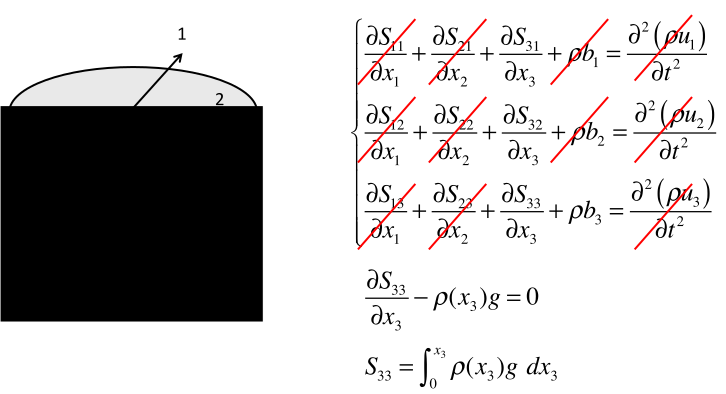
\includegraphics[scale=0.45]{.././Figures/split/4-7.pdf}%
\lthtmlpictureZ
\lthtmlcheckvsize\clearpage}

{\newpage\clearpage
\lthtmlinlinemathA{tex2html_wrap_inline21881}%
$ S_{11}$%
\lthtmlindisplaymathZ
\lthtmlcheckvsize\clearpage}

{\newpage\clearpage
\lthtmlinlinemathA{tex2html_wrap_inline21883}%
$ S_{22}$%
\lthtmlindisplaymathZ
\lthtmlcheckvsize\clearpage}

\stepcounter{subsection}
{\newpage\clearpage
\lthtmlinlinemathA{tex2html_wrap_inline21886}%
$ \uline{t}$%
\lthtmlindisplaymathZ
\lthtmlcheckvsize\clearpage}

{\newpage\clearpage
\lthtmlinlinemathA{tex2html_wrap_inline21890}%
$ \uline{b}$%
\lthtmlindisplaymathZ
\lthtmlcheckvsize\clearpage}

{\newpage\clearpage
\lthtmlpictureA{tex2html_wrap21892}%
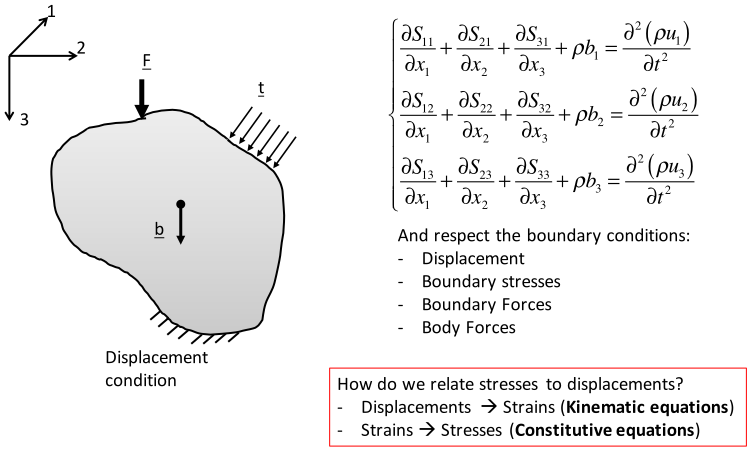
\includegraphics[scale=0.55]{.././Figures/split/4-8.pdf}%
\lthtmlpictureZ
\lthtmlcheckvsize\clearpage}

\stepcounter{section}
{\newpage\clearpage
\lthtmlpictureA{tex2html_wrap21898}%
\includegraphics[scale=0.65]{.././Figures/split/4-9.pdf}%
\lthtmlpictureZ
\lthtmlcheckvsize\clearpage}

{\newpage\clearpage
\lthtmlinlinemathA{tex2html_wrap_indisplay21905}%
$\displaystyle \varepsilon_{11} = \frac{\Delta u_1}{\Delta x_1}$%
\lthtmlindisplaymathZ
\lthtmlcheckvsize\clearpage}

{\newpage\clearpage
\lthtmlinlinemathA{tex2html_wrap_indisplay21907}%
$\displaystyle \varepsilon_{22} = \frac{\Delta u_2}{\Delta x_2}$%
\lthtmlindisplaymathZ
\lthtmlcheckvsize\clearpage}

{\newpage\clearpage
\lthtmlinlinemathA{tex2html_wrap_inline21909}%
$ \pi - \left[ \pi - \arctan(\Delta u_1 / \Delta x_2) + \arctan(\Delta u_2 / \Delta x_1) \right] $%
\lthtmlindisplaymathZ
\lthtmlcheckvsize\clearpage}

{\newpage\clearpage
\lthtmlinlinemathA{tex2html_wrap_inline21911}%
$ \arctan(x/y) \sim x/y$%
\lthtmlindisplaymathZ
\lthtmlcheckvsize\clearpage}

{\newpage\clearpage
\lthtmlinlinemathA{tex2html_wrap_indisplay21913}%
$\displaystyle \varepsilon_{12} = \frac{1}{2} \left( \frac{\Delta u_1}{\Delta x_2} + \frac{\Delta u_2}{\Delta x_1} \right)$%
\lthtmlindisplaymathZ
\lthtmlcheckvsize\clearpage}

{\newpage\clearpage
\lthtmlpictureA{tex2html_wrap21915}%
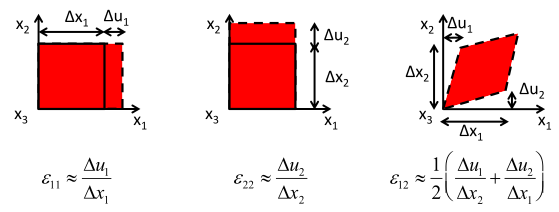
\includegraphics[scale=0.65]{.././Figures/split/4-10.pdf}%
\lthtmlpictureZ
\lthtmlcheckvsize\clearpage}

{\newpage\clearpage
\lthtmlinlinemathA{tex2html_wrap_inline21920}%
$ x_i$%
\lthtmlindisplaymathZ
\lthtmlcheckvsize\clearpage}

{\newpage\clearpage
\lthtmldisplayA{displaymath21922}%
\begin{displaymath}\uuline{\varepsilon} =
\left[
\begin{array}{ccc}
\cfrac{\partial u_1}{\partial x_1} & \cfrac{1}{2} \left( \cfrac{\partial u_1}{\partial x_2} + \cfrac{\partial u_2}{\partial x_1} \right) &  \cfrac{1}{2} \left( \cfrac{\partial u_1}{\partial x_3} + \cfrac{\partial u_3}{\partial x_1} \right)\\
\cfrac{1}{2} \left( \cfrac{\partial u_2}{\partial x_1} + \cfrac{\partial u_1}{\partial x_2} \right) & \cfrac{\partial u_2}{\partial x_2} & \cfrac{1}{2} \left( \cfrac{\partial u_2}{\partial x_3} + \cfrac{\partial u_3}{\partial x_2} \right)\\
\cfrac{1}{2} \left( \cfrac{\partial u_3}{\partial x_1} + \cfrac{\partial u_1}{\partial x_3} \right) &  \cfrac{1}{2} \left( \cfrac{\partial u_3}{\partial x_2} + \cfrac{\partial u_2}{\partial x_3} \right) & \cfrac{\partial u_3}{\partial x_3}
\end{array}
\right] =
\left[
\begin{array}{ccc}
\varepsilon_{11} & \varepsilon_{12}  &  \varepsilon_{13} \\
\varepsilon_{21} & \varepsilon_{22}  &  \varepsilon_{23} \\
\varepsilon_{31} & \varepsilon_{32}  &  \varepsilon_{33}
\end{array}
\right]\end{displaymath}%
\lthtmldisplayZ
\lthtmlcheckvsize\clearpage}

{\newpage\clearpage
\lthtmlinlinemathA{tex2html_wrap_indisplay21924}%
$\displaystyle \varepsilon_{vol} = \varepsilon_{11} + \varepsilon_{22} + \varepsilon_{33}$%
\lthtmlindisplaymathZ
\lthtmlcheckvsize\clearpage}

{\newpage\clearpage
\lthtmlinlinemathA{tex2html_wrap_inline21926}%
$ \Delta x_1 \Delta x_2 \Delta x_3$%
\lthtmlindisplaymathZ
\lthtmlcheckvsize\clearpage}

{\newpage\clearpage
\lthtmlinlinemathA{tex2html_wrap_inline21928}%
$ \Delta V$%
\lthtmlindisplaymathZ
\lthtmlcheckvsize\clearpage}

{\newpage\clearpage
\lthtmlinlinemathA{tex2html_wrap_inline21930}%
$ V_0$%
\lthtmlindisplaymathZ
\lthtmlcheckvsize\clearpage}

{\newpage\clearpage
\lthtmlinlinemathA{tex2html_wrap_indisplay21932}%
$\displaystyle \varepsilon_{vol} =  \frac{\Delta V}{V_0}
$%
\lthtmlindisplaymathZ
\lthtmlcheckvsize\clearpage}

{\newpage\clearpage
\lthtmlinlinemathA{tex2html_wrap_inline21934}%
$ \mathrm{d} x_1 \mathrm{d} x_2 \mathrm{d} x_3$%
\lthtmlindisplaymathZ
\lthtmlcheckvsize\clearpage}

{\newpage\clearpage
\lthtmlinlinemathA{tex2html_wrap_inline21936}%
$ (\mathrm{d} x_1 + \mathrm{d}u_1)(\mathrm{d} x_2 + \mathrm{d}u_2)(\mathrm{d} x_3 + \mathrm{d} u_3)$%
\lthtmlindisplaymathZ
\lthtmlcheckvsize\clearpage}

{\newpage\clearpage
\lthtmlinlinemathA{tex2html_wrap_indisplay21938}%
$\displaystyle \varepsilon_{vol} =  \frac{[(\mathrm{d} x_1 + \mathrm{d}u_1)(\mathrm{d} x_2 + \mathrm{d}u_2)(\mathrm{d} x_3 + \mathrm{d}u_3) - (\mathrm{d} x_1 \mathrm{d} x_2 \mathrm{d} x_3)]}{(\mathrm{d} x_1 \mathrm{d} x_2 \mathrm{d} x_3)}
$%
\lthtmlindisplaymathZ
\lthtmlcheckvsize\clearpage}

{\newpage\clearpage
\lthtmlinlinemathA{tex2html_wrap_inline21940}%
$ \mathrm{d}u_i \mathrm{d}u_j$%
\lthtmlindisplaymathZ
\lthtmlcheckvsize\clearpage}

{\newpage\clearpage
\lthtmlinlinemathA{tex2html_wrap_inline21942}%
$ \mathrm{d}u_1 \mathrm{d}u_2 \mathrm{d}u_3$%
\lthtmlindisplaymathZ
\lthtmlcheckvsize\clearpage}

{\newpage\clearpage
\lthtmlinlinemathA{tex2html_wrap_inline21944}%
$ \mathrm{d}u_i$%
\lthtmlindisplaymathZ
\lthtmlcheckvsize\clearpage}

{\newpage\clearpage
\lthtmlinlinemathA{tex2html_wrap_inline21946}%
$ \mathrm{d}u_i << \mathrm{d}x_j $%
\lthtmlindisplaymathZ
\lthtmlcheckvsize\clearpage}

{\newpage\clearpage
\lthtmlinlinemathA{tex2html_wrap_indisplay21948}%
$\displaystyle \varepsilon_{vol} \sim  \frac{(\mathrm{d} x_1 \mathrm{d} x_2 \mathrm{d}u_3 + 
							 \mathrm{d} x_1 \mathrm{d} x_3 \mathrm{d}u_2 +
							 \mathrm{d} x_2 \mathrm{d} x_3 \mathrm{d}u_1)}
							 {(\mathrm{d} x_1 \mathrm{d} x_2 \mathrm{d} x_3)}
				=  \frac{\mathrm{d}u_1}{\mathrm{d} x_1} + 
				   \frac{\mathrm{d}u_2}{\mathrm{d} x_2} + 
				   \frac{\mathrm{d}u_3}{\mathrm{d} x_3} 
				= \varepsilon_{11} + \varepsilon_{22} + \varepsilon_{33} \: \: \blacksquare
$%
\lthtmlindisplaymathZ
\lthtmlcheckvsize\clearpage}

\stepcounter{section}
{\newpage\clearpage
\lthtmlpictureA{tex2html_wrap21951}%
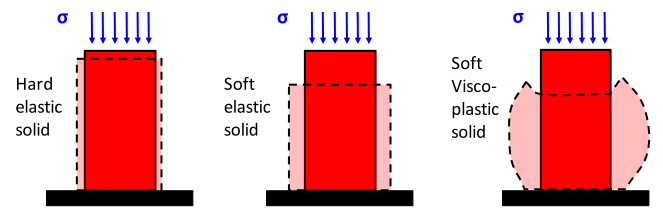
\includegraphics[scale=0.65]{.././Figures/split/4-12.pdf}%
\lthtmlpictureZ
\lthtmlcheckvsize\clearpage}

{\newpage\clearpage
\lthtmlinlinemathA{tex2html_wrap_inline21956}%
$ F$%
\lthtmlindisplaymathZ
\lthtmlcheckvsize\clearpage}

{\newpage\clearpage
\lthtmlinlinemathA{tex2html_wrap_inline21958}%
$ \Delta x$%
\lthtmlindisplaymathZ
\lthtmlcheckvsize\clearpage}

{\newpage\clearpage
\lthtmlinlinemathA{tex2html_wrap_indisplay21962}%
$\displaystyle F = k \Delta x$%
\lthtmlindisplaymathZ
\lthtmlcheckvsize\clearpage}

{\newpage\clearpage
\lthtmlinlinemathA{tex2html_wrap_inline21974}%
$ E$%
\lthtmlindisplaymathZ
\lthtmlcheckvsize\clearpage}

{\newpage\clearpage
\lthtmlinlinemathA{tex2html_wrap_indisplay21976}%
$\displaystyle \frac{F}{A} = E \frac{\Delta x}{L}$%
\lthtmlindisplaymathZ
\lthtmlcheckvsize\clearpage}

{\newpage\clearpage
\lthtmlinlinemathA{tex2html_wrap_inline21978}%
$ \sigma$%
\lthtmlindisplaymathZ
\lthtmlcheckvsize\clearpage}

{\newpage\clearpage
\lthtmlinlinemathA{tex2html_wrap_inline21980}%
$ \varepsilon$%
\lthtmlindisplaymathZ
\lthtmlcheckvsize\clearpage}

{\newpage\clearpage
\lthtmlinlinemathA{tex2html_wrap_indisplay21982}%
$\displaystyle \sigma = E \varepsilon$%
\lthtmlindisplaymathZ
\lthtmlcheckvsize\clearpage}

{\newpage\clearpage
\lthtmlinlinemathA{tex2html_wrap_inline21984}%
$ \uuline{\sigma}$%
\lthtmlindisplaymathZ
\lthtmlcheckvsize\clearpage}

{\newpage\clearpage
\lthtmlinlinemathA{tex2html_wrap_inline21986}%
$ \uuline{\varepsilon}$%
\lthtmlindisplaymathZ
\lthtmlcheckvsize\clearpage}

{\newpage\clearpage
\lthtmlinlinemathA{tex2html_wrap_inline21988}%
$ \uuline{C}$%
\lthtmlindisplaymathZ
\lthtmlcheckvsize\clearpage}

{\newpage\clearpage
\lthtmlinlinemathA{tex2html_wrap_indisplay21990}%
$\displaystyle \uuline{\sigma} = \uuline{C} \: \uuline{\varepsilon}$%
\lthtmlindisplaymathZ
\lthtmlcheckvsize\clearpage}

{\newpage\clearpage
\lthtmlpictureA{tex2html_wrap21992}%
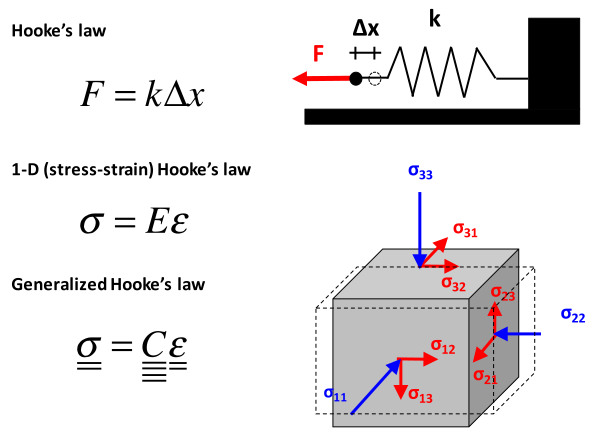
\includegraphics[scale=0.50]{.././Figures/split/4-13.pdf}%
\lthtmlpictureZ
\lthtmlcheckvsize\clearpage}

\stepcounter{subsection}
{\newpage\clearpage
\lthtmlinlinemathA{tex2html_wrap_inline22000}%
$ \sigma_{33}$%
\lthtmlindisplaymathZ
\lthtmlcheckvsize\clearpage}

{\newpage\clearpage
\lthtmlinlinemathA{tex2html_wrap_inline22006}%
$ \varepsilon_{33}$%
\lthtmlindisplaymathZ
\lthtmlcheckvsize\clearpage}

{\newpage\clearpage
\lthtmlinlinemathA{tex2html_wrap_indisplay22008}%
$\displaystyle E = \frac{\sigma_{33}}{\varepsilon_{33}}$%
\lthtmlindisplaymathZ
\lthtmlcheckvsize\clearpage}

{\newpage\clearpage
\lthtmlinlinemathA{tex2html_wrap_inline22010}%
$ \varepsilon_{11}$%
\lthtmlindisplaymathZ
\lthtmlcheckvsize\clearpage}

{\newpage\clearpage
\lthtmlinlinemathA{tex2html_wrap_inline22012}%
$ \varepsilon_{22}$%
\lthtmlindisplaymathZ
\lthtmlcheckvsize\clearpage}

{\newpage\clearpage
\lthtmlinlinemathA{tex2html_wrap_indisplay22016}%
$\displaystyle \nu = -\frac{\varepsilon_{11}}{\varepsilon_{33}}$%
\lthtmlindisplaymathZ
\lthtmlcheckvsize\clearpage}

{\newpage\clearpage
\lthtmlpictureA{tex2html_wrap22018}%
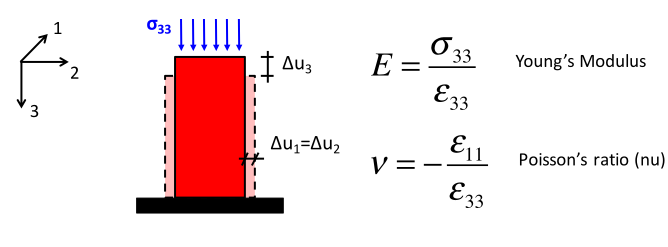
\includegraphics[scale=0.65]{.././Figures/split/4-14.pdf}%
\lthtmlpictureZ
\lthtmlcheckvsize\clearpage}

{\newpage\clearpage
\lthtmlinlinemathA{tex2html_wrap_inline22023}%
$ \sigma_a$%
\lthtmlindisplaymathZ
\lthtmlcheckvsize\clearpage}

{\newpage\clearpage
\lthtmlinlinemathA{tex2html_wrap_inline22025}%
$ \varepsilon_a$%
\lthtmlindisplaymathZ
\lthtmlcheckvsize\clearpage}

{\newpage\clearpage
\lthtmlinlinemathA{tex2html_wrap_indisplay22037}%
$\displaystyle \sigma_a = 3000$%
\lthtmlindisplaymathZ
\lthtmlcheckvsize\clearpage}

{\newpage\clearpage
\lthtmlinlinemathA{tex2html_wrap_indisplay22038}%
$\displaystyle = 3000 \frac{1}{145}$%
\lthtmlindisplaymathZ
\lthtmlcheckvsize\clearpage}

{\newpage\clearpage
\lthtmlinlinemathA{tex2html_wrap_indisplay22039}%
$\displaystyle = 20.7$%
\lthtmlindisplaymathZ
\lthtmlcheckvsize\clearpage}

{\newpage\clearpage
\lthtmlinlinemathA{tex2html_wrap_indisplay22041}%
$\displaystyle \varepsilon_a(1$%
\lthtmlindisplaymathZ
\lthtmlcheckvsize\clearpage}

{\newpage\clearpage
\lthtmlinlinemathA{tex2html_wrap_indisplay22042}%
$\displaystyle ) = \frac{\sigma_a}{E} = \frac{20.7 \text{ MPa}}{1000 \text{ MPa}} = 0.0207 = 2.07 \%
$%
\lthtmlindisplaymathZ
\lthtmlcheckvsize\clearpage}

{\newpage\clearpage
\lthtmlinlinemathA{tex2html_wrap_indisplay22044}%
$\displaystyle \varepsilon_a(10$%
\lthtmlindisplaymathZ
\lthtmlcheckvsize\clearpage}

{\newpage\clearpage
\lthtmlinlinemathA{tex2html_wrap_indisplay22045}%
$\displaystyle ) = \frac{\sigma_a}{E} = \frac{20.7 \text{ MPa}}{10000 \text{ MPa}} = 0.00207 = 0.207 \%
$%
\lthtmlindisplaymathZ
\lthtmlcheckvsize\clearpage}

{\newpage\clearpage
\lthtmlinlinemathA{tex2html_wrap_indisplay22047}%
$\displaystyle \varepsilon_a(50$%
\lthtmlindisplaymathZ
\lthtmlcheckvsize\clearpage}

{\newpage\clearpage
\lthtmlinlinemathA{tex2html_wrap_indisplay22048}%
$\displaystyle ) = \frac{\sigma_a}{E} = \frac{20.7 \text{ MPa}}{50000 \text{ MPa}} = 0.00041 = 0.041 \%
$%
\lthtmlindisplaymathZ
\lthtmlcheckvsize\clearpage}

\stepcounter{subsection}
{\newpage\clearpage
\lthtmldisplayA{displaymath22053}%
\begin{displaymath}\left\lbrace
\begin{array}{rcl}
\varepsilon_{11} & = & +\cfrac{1}{E} \: \sigma_{11} -\cfrac{\nu}{E} \: \sigma_{22} -\cfrac{\nu}{E} \: \sigma_{33}\\
\varepsilon_{22} & = &  -\cfrac{\nu}{E} \: \sigma_{11} +\cfrac{1}{E} \: \sigma_{22} - \cfrac{\nu}{E} \: \sigma_{33}\\
\varepsilon_{33} & = & -\cfrac{\nu}{E} \: \sigma_{11} -\cfrac{\nu}{E} \: \sigma_{22} + \cfrac{1}{E} \: \sigma_{33}
\end{array}
\right.\end{displaymath}%
\lthtmldisplayZ
\lthtmlcheckvsize\clearpage}

{\newpage\clearpage
\lthtmlinlinemathA{tex2html_wrap_inline22055}%
$ \varepsilon_{ij}$%
\lthtmlindisplaymathZ
\lthtmlcheckvsize\clearpage}

{\newpage\clearpage
\lthtmlinlinemathA{tex2html_wrap_inline22057}%
$ G=E/[2(1+\nu)]$%
\lthtmlindisplaymathZ
\lthtmlcheckvsize\clearpage}

{\newpage\clearpage
\lthtmldisplayA{displaymath22059}%
\begin{displaymath}\left\lbrace
\begin{array}{rcl}
2 \varepsilon_{12} & = & \cfrac{1}{G} \: \sigma_{12}\\
2 \varepsilon_{13} & = & \cfrac{1}{G} \: \sigma_{13}\\
2 \varepsilon_{23} & = & \cfrac{1}{G} \: \sigma_{23}
\end{array}
\right.\end{displaymath}%
\lthtmldisplayZ
\lthtmlcheckvsize\clearpage}

{\newpage\clearpage
\lthtmlinlinemathA{tex2html_wrap_inline22065}%
$ \uuline{D}$%
\lthtmlindisplaymathZ
\lthtmlcheckvsize\clearpage}

{\newpage\clearpage
\lthtmlinlinemathA{tex2html_wrap_indisplay22067}%
$\displaystyle \uuline{\varepsilon} = \uuline{D} \: \uuline{\sigma}$%
\lthtmlindisplaymathZ
\lthtmlcheckvsize\clearpage}

{\newpage\clearpage
\lthtmlinlinemathA{tex2html_wrap_inline22069}%
$ 6 \times 1$%
\lthtmlindisplaymathZ
\lthtmlcheckvsize\clearpage}

{\newpage\clearpage
\lthtmlinlinemathA{tex2html_wrap_inline22073}%
$ 6 \times 6$%
\lthtmlindisplaymathZ
\lthtmlcheckvsize\clearpage}

{\newpage\clearpage
\lthtmldisplayA{displaymath22079}%
\begin{displaymath}%compliance matrix
	\left[
\begin{array} {c}
\varepsilon_{11} \cfrac{}{}\\
\varepsilon_{22} \cfrac{}{}\\
\varepsilon_{33} \cfrac{}{}\\
2 \varepsilon_{12} \cfrac{}{}\\
2 \varepsilon_{13} \cfrac{}{}\\
2 \varepsilon_{23} \cfrac{}{}
\end{array}
\right] =
\left[
\begin{array}{cccccc}
+\cfrac{1}{E} & -\cfrac{\nu}{E} & -\cfrac{\nu}{E} & 0 & 0 & 0\\
-\cfrac{\nu}{E} & +\cfrac{1}{E} & -\cfrac{\nu}{E} & 0 & 0 & 0\\
-\cfrac{\nu}{E} & -\cfrac{\nu}{E} & +\cfrac{1}{E} & 0 & 0 & 0\\
0 & 0 & 0 & \cfrac{2(1+\nu)}{E} & 0 & 0 \\
0 & 0 & 0 & 0 & \cfrac{2(1+\nu)}{E} & 0 \\
0 & 0 & 0 & 0 & 0 & \cfrac{2(1+\nu)}{E}
\end{array}
\right] \:
\left[
\begin{array} {c}
\sigma_{11} \cfrac{}{}\\
\sigma_{22} \cfrac{}{}\\
\sigma_{33} \cfrac{}{}\\
\sigma_{12} \cfrac{}{}\\
\sigma_{13} \cfrac{}{}\\
\sigma_{23} \cfrac{}{}
\end{array}
\right]\end{displaymath}%
\lthtmldisplayZ
\lthtmlcheckvsize\clearpage}

{\newpage\clearpage
\lthtmlinlinemathA{tex2html_wrap_inline22081}%
$ \uuline{\sigma} = [0,0,\sigma_{33},0,0,0]^T$%
\lthtmlindisplaymathZ
\lthtmlcheckvsize\clearpage}

{\newpage\clearpage
\lthtmlinlinemathA{tex2html_wrap_inline22083}%
$ \uuline{D} \: \uuline{\sigma}$%
\lthtmlindisplaymathZ
\lthtmlcheckvsize\clearpage}

{\newpage\clearpage
\lthtmlinlinemathA{tex2html_wrap_indisplay22085}%
$\displaystyle \uuline{\varepsilon} = \left [ -\cfrac{\nu}{E} \: \sigma_{33},-\cfrac{\nu}{E} \: \sigma_{33},\cfrac{1}{E} \: \sigma_{33},0,0,0 \right]^T $%
\lthtmlindisplaymathZ
\lthtmlcheckvsize\clearpage}

{\newpage\clearpage
\lthtmlinlinemathA{tex2html_wrap_inline22089}%
$ \nu$%
\lthtmlindisplaymathZ
\lthtmlcheckvsize\clearpage}

{\newpage\clearpage
\lthtmlinlinemathA{tex2html_wrap_inline22091}%
$ \uuline{C} = \uuline{D}^{-1}$%
\lthtmlindisplaymathZ
\lthtmlcheckvsize\clearpage}

{\newpage\clearpage
\lthtmldisplayA{displaymath22093}%
\begin{displaymath}%stiffness matrix
	\left[
\begin{array} {c}
\sigma_{11} \\
\sigma_{22} \\
\sigma_{33} \\
\sigma_{12} \cfrac{}{} \\
\sigma_{13} \cfrac{}{} \\
\sigma_{23} \cfrac{}{}
\end{array}
\right]
= \cfrac{E}{(1+\nu)(1-2\nu)}
\left[
\begin{array}{cccccc}
1-\nu & \nu & \nu & 0 & 0 & 0\\
\nu & 1-\nu & \nu & 0 & 0 & 0\\
\nu & \nu & 1-\nu & 0 & 0 & 0\\
0 & 0 & 0 & \cfrac{(1-2\nu)}{2} & 0 & 0 \\
0 & 0 & 0 & 0 & \cfrac{(1-2\nu)}{2} & 0 \\
0 & 0 & 0 & 0 & 0 & \cfrac{(1-2\nu)}{2}
\end{array}
\right]
\:
\left[
\begin{array} {c}
\varepsilon_{11} \\
\varepsilon_{22} \\
\varepsilon_{33} \\
2 \varepsilon_{12} \cfrac{}{} \\
2 \varepsilon_{13}  \cfrac{}{}\\
2 \varepsilon_{23} \cfrac{}{}
\end{array}
\right]\end{displaymath}%
\lthtmldisplayZ
\lthtmlcheckvsize\clearpage}

{\newpage\clearpage
\lthtmlinlinemathA{tex2html_wrap_inline22095}%
$ \lambda$%
\lthtmlindisplaymathZ
\lthtmlcheckvsize\clearpage}

{\newpage\clearpage
\lthtmlinlinemathA{tex2html_wrap_indisplay22103}%
$\displaystyle \sigma_{11}  = \cfrac{E}{(1+\nu)(1-2\nu)}
\left[ (1-\nu) \varepsilon_{11} + \nu \varepsilon_{22} + \nu \varepsilon_{33} \right]$%
\lthtmlindisplaymathZ
\lthtmlcheckvsize\clearpage}

{\newpage\clearpage
\lthtmlinlinemathA{tex2html_wrap_indisplay22105}%
$\displaystyle \sigma_{11}  = \cfrac{\nu E}{(1+\nu)(1-2\nu)}
(\varepsilon_{11} + \varepsilon_{22} + \varepsilon_{33})
+  \cfrac{\nu E}{(1+\nu)(1-2\nu)} \left( -1 + \cfrac{1-\nu}{\nu} \right) \varepsilon_{11}$%
\lthtmlindisplaymathZ
\lthtmlcheckvsize\clearpage}

{\newpage\clearpage
\lthtmlinlinemathA{tex2html_wrap_indisplay22107}%
$\displaystyle \lambda = \cfrac{\nu E}{(1+\nu)(1-2\nu)}$%
\lthtmlindisplaymathZ
\lthtmlcheckvsize\clearpage}

{\newpage\clearpage
\lthtmlinlinemathA{tex2html_wrap_indisplay22109}%
$\displaystyle 2\mu =  \cfrac{\nu E}{(1+\nu)(1-2\nu)} \left( -1 + \cfrac{1-\nu}{\nu} \right) = \cfrac{E}{(1+\nu)}$%
\lthtmlindisplaymathZ
\lthtmlcheckvsize\clearpage}

{\newpage\clearpage
\lthtmlinlinemathA{tex2html_wrap_inline22111}%
$ \mu = G$%
\lthtmlindisplaymathZ
\lthtmlcheckvsize\clearpage}

{\newpage\clearpage
\lthtmldisplayA{displaymath22113}%
\begin{displaymath}\left\lbrace
\begin{array}{rcl}
\sigma_{11} & = & (\lambda + 2 \mu) \: \varepsilon_{11} + \lambda \: \varepsilon_{22} + \lambda \: \varepsilon_{33}\\
\sigma_{22} & = & \lambda \: \varepsilon_{11} + (\lambda + 2 \mu) \: \varepsilon_{22} + \lambda \: \varepsilon_{33}\\
\sigma_{33} & = & \lambda \: \varepsilon_{11} + \lambda \: \varepsilon_{22} + (\lambda + 2 \mu) \: \varepsilon_{33}\\
\sigma_{12} & = & 2 \mu \: \varepsilon_{12}\\
\sigma_{13} & = & 2 \mu \: \varepsilon_{13}\\
\sigma_{23} & = & 2 \mu \: \varepsilon_{23}\\
\end{array}
\right. \text{.}\end{displaymath}%
\lthtmldisplayZ
\lthtmlcheckvsize\clearpage}

{\newpage\clearpage
\lthtmldisplayA{displaymath22115}%
\begin{displaymath}%compliance matrix
	\left[
\begin{array} {c}
\sigma_{11} \\
\sigma_{22} \\
\sigma_{33} \\
\sigma_{12} \\
\sigma_{13} \\
\sigma_{23}
\end{array}
\right]
=
\left[
\begin{array}{cccccc}
\lambda + 2\mu & \lambda & \lambda & 0 & 0 & 0\\
\lambda & \lambda + 2 \mu & \lambda & 0 & 0 & 0\\
\lambda & \lambda & \lambda + 2 \mu & 0 & 0 & 0\\
0 & 0 & 0 & \mu & 0 & 0 \\
0 & 0 & 0 & 0 & \mu & 0 \\
0 & 0 & 0 & 0 & 0 & \mu
\end{array}
\right]
\:
\left[
\begin{array} {c}
\varepsilon_{11} \\
\varepsilon_{22} \\
\varepsilon_{33} \\
2 \varepsilon_{12} \\
2 \varepsilon_{13} \\
2 \varepsilon_{23}
\end{array}
\right] \: \: \blacksquare\end{displaymath}%
\lthtmldisplayZ
\lthtmlcheckvsize\clearpage}

{\newpage\clearpage
\lthtmlinlinemathA{tex2html_wrap_inline22121}%
$ K$%
\lthtmlindisplaymathZ
\lthtmlcheckvsize\clearpage}

{\newpage\clearpage
\lthtmlinlinemathA{tex2html_wrap_inline22123}%
$ G$%
\lthtmlindisplaymathZ
\lthtmlcheckvsize\clearpage}

{\newpage\clearpage
\lthtmlpictureA{tex2html_wrap22125}%
\includegraphics[scale=0.55]{.././Figures/split/4-21.pdf}%
\lthtmlpictureZ
\lthtmlcheckvsize\clearpage}

\stepcounter{subsection}
{\newpage\clearpage
\lthtmlinlinemathA{tex2html_wrap_inline22131}%
$ \uuline{\varepsilon} = \uuline{D} \: \uuline{S}$%
\lthtmlindisplaymathZ
\lthtmlcheckvsize\clearpage}

{\newpage\clearpage
\lthtmlinlinemathA{tex2html_wrap_indisplay22133}%
$\displaystyle \uuline{\varepsilon} = \uuline{D} \: (\uuline{S} - P_p \uuline{I})  = \uuline{D} \: \uuline{\sigma}$%
\lthtmlindisplaymathZ
\lthtmlcheckvsize\clearpage}

{\newpage\clearpage
\lthtmlpictureA{tex2html_wrap22135}%
\includegraphics[scale=0.55]{.././Figures/split/4-26.pdf}%
\lthtmlpictureZ
\lthtmlcheckvsize\clearpage}

{\newpage\clearpage
\lthtmlinlinemathA{tex2html_wrap_indisplay22142}%
$\displaystyle \uuline{\varepsilon} = \uuline{D} \: (\uuline{S} - \alpha P_p \uuline{I})$%
\lthtmlindisplaymathZ
\lthtmlcheckvsize\clearpage}

{\newpage\clearpage
\lthtmlinlinemathA{tex2html_wrap_inline22144}%
$ \alpha \sim 1$%
\lthtmlindisplaymathZ
\lthtmlcheckvsize\clearpage}

{\newpage\clearpage
\lthtmlinlinemathA{tex2html_wrap_inline22146}%
$ \alpha \sim 0.5$%
\lthtmlindisplaymathZ
\lthtmlcheckvsize\clearpage}

\stepcounter{subsection}
{\newpage\clearpage
\lthtmlinlinemathA{tex2html_wrap_inline22149}%
$ S_v = S_{33}$%
\lthtmlindisplaymathZ
\lthtmlcheckvsize\clearpage}

{\newpage\clearpage
\lthtmlinlinemathA{tex2html_wrap_indisplay22153}%
$\displaystyle \sigma_v(z) = S_v(z) - P_p$%
\lthtmlindisplaymathZ
\lthtmlcheckvsize\clearpage}

{\newpage\clearpage
\lthtmlinlinemathA{tex2html_wrap_inline22155}%
$ \varepsilon_{11}=\varepsilon_{22}$%
\lthtmlindisplaymathZ
\lthtmlcheckvsize\clearpage}

{\newpage\clearpage
\lthtmlinlinemathA{tex2html_wrap_inline22161}%
$ \uuline{\varepsilon} = [0,0,\varepsilon_{33},0,0,0]^T$%
\lthtmlindisplaymathZ
\lthtmlcheckvsize\clearpage}

{\newpage\clearpage
\lthtmlinlinemathA{tex2html_wrap_inline22163}%
$ \uuline{\sigma} = \uuline{D} \: \uuline{\varepsilon}$%
\lthtmlindisplaymathZ
\lthtmlcheckvsize\clearpage}

{\newpage\clearpage
\lthtmldisplayA{displaymath22165}%
\begin{displaymath}\left\lbrace
\begin{array}{l}
\sigma_{11} = \sigma_{22} =
\frac{\nu E}{(1+\nu)(1-2\nu)} \varepsilon_{33}  \\
\sigma_{33} = \frac{(1-\nu) E}{(1+\nu)(1-2\nu)} 		 			\varepsilon_{33}
\end{array}
\right.\end{displaymath}%
\lthtmldisplayZ
\lthtmlcheckvsize\clearpage}

{\newpage\clearpage
\lthtmlinlinemathA{tex2html_wrap_inline22171}%
$ \sigma_{11}$%
\lthtmlindisplaymathZ
\lthtmlcheckvsize\clearpage}

{\newpage\clearpage
\lthtmlinlinemathA{tex2html_wrap_inline22173}%
$ \sigma_{22}$%
\lthtmlindisplaymathZ
\lthtmlcheckvsize\clearpage}

{\newpage\clearpage
\lthtmlinlinemathA{tex2html_wrap_indisplay22175}%
$\displaystyle \sigma_{11} = \sigma_{22} = \frac{\nu}{1-\nu} \sigma_{33}$%
\lthtmlindisplaymathZ
\lthtmlcheckvsize\clearpage}

{\newpage\clearpage
\lthtmlinlinemathA{tex2html_wrap_indisplay22177}%
$\displaystyle \sigma_{h} = \frac{\nu}{1-\nu} \sigma_{v}$%
\lthtmlindisplaymathZ
\lthtmlcheckvsize\clearpage}

{\newpage\clearpage
\lthtmlinlinemathA{tex2html_wrap_inline22179}%
$ \nu \sim 0.25$%
\lthtmlindisplaymathZ
\lthtmlcheckvsize\clearpage}

{\newpage\clearpage
\lthtmlinlinemathA{tex2html_wrap_inline22181}%
$ \nu/(1-\nu) \sim 1/3 $%
\lthtmlindisplaymathZ
\lthtmlcheckvsize\clearpage}

{\newpage\clearpage
\lthtmlinlinemathA{tex2html_wrap_inline22183}%
$ \nu \rightarrow 0.5$%
\lthtmlindisplaymathZ
\lthtmlcheckvsize\clearpage}

{\newpage\clearpage
\lthtmlinlinemathA{tex2html_wrap_inline22185}%
$ \nu/(1-\nu) \rightarrow 1$%
\lthtmlindisplaymathZ
\lthtmlcheckvsize\clearpage}

{\newpage\clearpage
\lthtmlinlinemathA{tex2html_wrap_inline22187}%
$ \nu \sim 0.5$%
\lthtmlindisplaymathZ
\lthtmlcheckvsize\clearpage}

{\newpage\clearpage
\lthtmlinlinemathA{tex2html_wrap_inline22193}%
$ S_{11} = \sigma_{11} + P_p$%
\lthtmlindisplaymathZ
\lthtmlcheckvsize\clearpage}

{\newpage\clearpage
\lthtmlinlinemathA{tex2html_wrap_inline22195}%
$ S_{22} = \sigma_{22} + P_p$%
\lthtmlindisplaymathZ
\lthtmlcheckvsize\clearpage}

{\newpage\clearpage
\lthtmlinlinemathA{tex2html_wrap_inline22221}%
$ \varepsilon_{11} \neq \varepsilon_{22} \neq 0$%
\lthtmlindisplaymathZ
\lthtmlcheckvsize\clearpage}

{\newpage\clearpage
\lthtmlinlinemathA{tex2html_wrap_inline22223}%
$ \uuline{\sigma} = \uuline{C} \: \uuline{\varepsilon}$%
\lthtmlindisplaymathZ
\lthtmlcheckvsize\clearpage}

{\newpage\clearpage
\lthtmlinlinemathA{tex2html_wrap_inline22225}%
$ \uuline{\varepsilon} = [\varepsilon_{11},\varepsilon_{22},\varepsilon_{33},0,0,0]^T$%
\lthtmlindisplaymathZ
\lthtmlcheckvsize\clearpage}

{\newpage\clearpage
\lthtmldisplayA{displaymath22227}%
\begin{displaymath}\left\lbrace
\begin{array}{l}
\sigma_{11} =
\cfrac{(1-\nu) E}{(1+\nu)(1-2\nu)} \varepsilon_{11}
+ \cfrac{\nu E}{(1+\nu)(1-2\nu)} \varepsilon_{22}
+ \cfrac{\nu E}{(1+\nu)(1-2\nu)} \varepsilon_{33} \\
\sigma_{22} =
\cfrac{\nu E}{(1+\nu)(1-2\nu)} \varepsilon_{11}
+ \cfrac{(1-\nu) E}{(1+\nu)(1-2\nu)} \varepsilon_{22}
+ \cfrac{\nu E}{(1+\nu)(1-2\nu)} \varepsilon_{33} \\
\sigma_{33} =
\cfrac{\nu E}{(1+\nu)(1-2\nu)} \varepsilon_{11}
+   \cfrac{\nu E}{(1+\nu)(1-2\nu)} \varepsilon_{22}
+	\cfrac{(1-\nu) E}{(1+\nu)(1-2\nu)} \varepsilon_{33}
\end{array}
\right.\end{displaymath}%
\lthtmldisplayZ
\lthtmlcheckvsize\clearpage}

{\newpage\clearpage
\lthtmldisplayA{displaymath22237}%
\begin{displaymath}\left\lbrace
\begin{array}{l}
\sigma_{11} =
\cfrac{\nu}{1-\nu} \sigma_{33} +
\cfrac{E}{1-\nu^2} \varepsilon_{11} +
\cfrac{\nu E}{1-\nu^2} \varepsilon_{22} \\
\sigma_{22} =
\cfrac{\nu}{1-\nu} \sigma_{33} +
\cfrac{\nu E}{1-\nu^2} \varepsilon_{11} +
\cfrac{E}{1-\nu^2} \varepsilon_{22} \\
\end{array}
\right.\end{displaymath}%
\lthtmldisplayZ
\lthtmlcheckvsize\clearpage}

{\newpage\clearpage
\lthtmlinlinemathA{tex2html_wrap_inline22241}%
$ \varepsilon_{hmin}$%
\lthtmlindisplaymathZ
\lthtmlcheckvsize\clearpage}

{\newpage\clearpage
\lthtmldisplayA{displaymath22243}%
\begin{displaymath}\left\lbrace
\begin{array}{l}
\sigma_{Hmax} =  \cfrac{\nu}{1-\nu} \sigma_{v} +
E' \varepsilon_{Hmax} +
\nu E'\varepsilon_{hmin}  \\
\sigma_{hmin} =  \cfrac{\nu}{1-\nu} \sigma_{v} +
\nu E' \varepsilon_{Hmax} +
E' \varepsilon_{hmin} \\
\end{array}
\right.\end{displaymath}%
\lthtmldisplayZ
\lthtmlcheckvsize\clearpage}

{\newpage\clearpage
\lthtmlinlinemathA{tex2html_wrap_inline22245}%
$ E' = \frac{E}{1-\nu^2}$%
\lthtmlindisplaymathZ
\lthtmlcheckvsize\clearpage}

{\newpage\clearpage
\lthtmlinlinemathA{tex2html_wrap_inline22261}%
$ \sigma_{hmin}$%
\lthtmlindisplaymathZ
\lthtmlcheckvsize\clearpage}

{\newpage\clearpage
\lthtmlinlinemathA{tex2html_wrap_inline22263}%
$ \sigma_{Hmax}$%
\lthtmlindisplaymathZ
\lthtmlcheckvsize\clearpage}

{\newpage\clearpage
\lthtmlinlinemathA{tex2html_wrap_inline22269}%
$ \mathrm{d}S_v/\mathrm{d}z = 23.8$%
\lthtmlindisplaymathZ
\lthtmlcheckvsize\clearpage}

{\newpage\clearpage
\lthtmlinlinemathA{tex2html_wrap_inline22271}%
$ \lambda_p = 0.7$%
\lthtmlindisplaymathZ
\lthtmlcheckvsize\clearpage}

{\newpage\clearpage
\lthtmlinlinemathA{tex2html_wrap_inline22275}%
$ \nu = 0.22$%
\lthtmlindisplaymathZ
\lthtmlcheckvsize\clearpage}

{\newpage\clearpage
\lthtmlinlinemathA{tex2html_wrap_inline22277}%
$ \varepsilon_{hmin} = 0$%
\lthtmlindisplaymathZ
\lthtmlcheckvsize\clearpage}

{\newpage\clearpage
\lthtmlinlinemathA{tex2html_wrap_inline22279}%
$ \varepsilon_{Hmax} = 0.0002$%
\lthtmlindisplaymathZ
\lthtmlcheckvsize\clearpage}

{\newpage\clearpage
\lthtmlinlinemathA{tex2html_wrap_indisplay22281}%
$\displaystyle S_v = 23.8 \frac{\text{MPa}}{\text{km}} \times \frac{1 \frac{\text{psi}}{\text{ft}}}{23 \frac{\text{MPa}}{\text{km}}} \times 7950 \text{ ft} = 8227 \text {psi}
$%
\lthtmlindisplaymathZ
\lthtmlcheckvsize\clearpage}

{\newpage\clearpage
\lthtmlinlinemathA{tex2html_wrap_indisplay22283}%
$\displaystyle P_p = \lambda_p S_v = 0.7 \times 8227$%
\lthtmlindisplaymathZ
\lthtmlcheckvsize\clearpage}

{\newpage\clearpage
\lthtmlinlinemathA{tex2html_wrap_indisplay22284}%
$\displaystyle \text {psi} = 5759 \text{ psi}
$%
\lthtmlindisplaymathZ
\lthtmlcheckvsize\clearpage}

{\newpage\clearpage
\lthtmlinlinemathA{tex2html_wrap_indisplay22286}%
$\displaystyle \sigma_v = S_v - P_p = 8227$%
\lthtmlindisplaymathZ
\lthtmlcheckvsize\clearpage}

{\newpage\clearpage
\lthtmlinlinemathA{tex2html_wrap_indisplay22287}%
$\displaystyle \text {psi} - 5759 \text{ psi} = 2468 \text{ psi}
$%
\lthtmlindisplaymathZ
\lthtmlcheckvsize\clearpage}

{\newpage\clearpage
\lthtmlinlinemathA{tex2html_wrap_indisplay22289}%
$\displaystyle E' = \frac{E}{1-\nu^2} = \frac{5 \times 10^6 \text{ psi}}{1-0.22^2} = 5.25 \times 10^6 \text{ psi}
$%
\lthtmlindisplaymathZ
\lthtmlcheckvsize\clearpage}

{\newpage\clearpage
\lthtmldisplayA{displaymath22291}%
\begin{displaymath}\left\lbrace
\begin{array}{l}
\sigma_{Hmax} =  \frac{\nu}{1-\nu} \sigma_{v} +
E' \varepsilon_{Hmax} +
\nu E'\varepsilon_{hmin} =
\frac{0.22}{1-0.22} 2468 \text{ psi} +
5.25 \times 10^6 \text{ psi} \times 0.0002 = 1745 \text{ psi}\\
\sigma_{hmin} =  \frac{\nu}{1-\nu} \sigma_{v} +
\nu E' \varepsilon_{Hmax} +
E' \varepsilon_{hmin} =
\frac{0.22}{1-0.22} 2468 \text{ psi} +
0.22 \times 5.25 \times 10^6 \text{ psi} \times 0.0002 = 927 \text{ psi}  \\
\end{array}
\right.\end{displaymath}%
\lthtmldisplayZ
\lthtmlcheckvsize\clearpage}

{\newpage\clearpage
\lthtmldisplayA{displaymath22293}%
\begin{displaymath}\left\lbrace
\begin{array}{l}
S_{Hmax} = \sigma_{Hmax} + P_p =  1745 \text{ psi} + 5759 \text{ psi} = 7504 \text{ psi}\\
S_{hmin} = \sigma_{hmin} + P_p =  927 \text{ psi} + 5759 \text{ psi} = 6686 \text{ psi}
\end{array}
\right. \: \: \blacksquare\end{displaymath}%
\lthtmldisplayZ
\lthtmlcheckvsize\clearpage}

\stepcounter{subsection}
{\newpage\clearpage
\lthtmlinlinemathA{tex2html_wrap_inline22296}%
$ C_{pp}$%
\lthtmlindisplaymathZ
\lthtmlcheckvsize\clearpage}

{\newpage\clearpage
\lthtmlinlinemathA{tex2html_wrap_indisplay22298}%
$\displaystyle \frac{\partial P_p}{\partial t}= \frac{k}{\mu C_t} \frac{\partial^2 P_p}{\partial x^2}$%
\lthtmlindisplaymathZ
\lthtmlcheckvsize\clearpage}

{\newpage\clearpage
\lthtmlinlinemathA{tex2html_wrap_inline22300}%
$ C_t = C_g S_g + C_w S_w + C_o S_o + C_{pp}$%
\lthtmlindisplaymathZ
\lthtmlcheckvsize\clearpage}

{\newpage\clearpage
\lthtmlinlinemathA{tex2html_wrap_inline22302}%
$ (C_g S_g + C_w S_w + C_o S_o)$%
\lthtmlindisplaymathZ
\lthtmlcheckvsize\clearpage}

{\newpage\clearpage
\lthtmlinlinemathA{tex2html_wrap_inline22308}%
$ V_p$%
\lthtmlindisplaymathZ
\lthtmlcheckvsize\clearpage}

{\newpage\clearpage
\lthtmlinlinemathA{tex2html_wrap_indisplay22310}%
$\displaystyle C_{pp} = \left. \frac{1}{V_p} \frac{\mathrm{d}V_p}{\mathrm{d}P_p} \right|_{S_v,\varepsilon_h}$%
\lthtmlindisplaymathZ
\lthtmlcheckvsize\clearpage}

{\newpage\clearpage
\lthtmlinlinemathA{tex2html_wrap_inline22314}%
$ \varepsilon_h$%
\lthtmlindisplaymathZ
\lthtmlcheckvsize\clearpage}

{\newpage\clearpage
\lthtmlinlinemathA{tex2html_wrap_inline22318}%
$ \mathrm{d}V_p$%
\lthtmlindisplaymathZ
\lthtmlcheckvsize\clearpage}

{\newpage\clearpage
\lthtmlinlinemathA{tex2html_wrap_inline22320}%
$ \mathrm{d}V_b$%
\lthtmlindisplaymathZ
\lthtmlcheckvsize\clearpage}

{\newpage\clearpage
\lthtmlinlinemathA{tex2html_wrap_indisplay22324}%
$\displaystyle C_{pp} = \frac{1}{\frac{V_p}{V_b}} \left( \frac{1}{V_b}  \left. \frac{\mathrm{d}V_b}{\mathrm{d}P_p} \right|_{S_v,\varepsilon_h} \right)$%
\lthtmlindisplaymathZ
\lthtmlcheckvsize\clearpage}

{\newpage\clearpage
\lthtmlinlinemathA{tex2html_wrap_inline22326}%
$ \phi = V_p/V_b$%
\lthtmlindisplaymathZ
\lthtmlcheckvsize\clearpage}

{\newpage\clearpage
\lthtmlinlinemathA{tex2html_wrap_inline22330}%
$ \varepsilon_{vol} = \mathrm{d}V_b/V_b$%
\lthtmlindisplaymathZ
\lthtmlcheckvsize\clearpage}

{\newpage\clearpage
\lthtmlinlinemathA{tex2html_wrap_indisplay22336}%
$\displaystyle C_{pp} = \frac{C_{bp}}{\phi}$%
\lthtmlindisplaymathZ
\lthtmlcheckvsize\clearpage}

{\newpage\clearpage
\lthtmlinlinemathA{tex2html_wrap_inline22338}%
$ C_{bp} \sim M^{-1}$%
\lthtmlindisplaymathZ
\lthtmlcheckvsize\clearpage}

{\newpage\clearpage
\lthtmlinlinemathA{tex2html_wrap_inline22340}%
$ M = (1-\nu) E / [(1+\nu)(1-2\nu)]$%
\lthtmlindisplaymathZ
\lthtmlcheckvsize\clearpage}

{\newpage\clearpage
\lthtmlinlinemathA{tex2html_wrap_indisplay22346}%
$\displaystyle C_{pp} = \frac{(1+\nu)(1-2\nu)}{(1-\nu) E \phi}$%
\lthtmlindisplaymathZ
\lthtmlcheckvsize\clearpage}

{\newpage\clearpage
\lthtmlinlinemathA{tex2html_wrap_inline22356}%
$ \times 10^{-6}$%
\lthtmlindisplaymathZ
\lthtmlcheckvsize\clearpage}

{\newpage\clearpage
\lthtmlinlinemathA{tex2html_wrap_inline22360}%
$ ^{-1} = \mu$%
\lthtmlindisplaymathZ
\lthtmlcheckvsize\clearpage}

{\newpage\clearpage
\lthtmlinlinemathA{tex2html_wrap_inline22362}%
$ \sim 2 \: \mu$%
\lthtmlindisplaymathZ
\lthtmlcheckvsize\clearpage}

{\newpage\clearpage
\lthtmlinlinemathA{tex2html_wrap_inline22364}%
$ \sim 30 \: \mu$%
\lthtmlindisplaymathZ
\lthtmlcheckvsize\clearpage}

{\newpage\clearpage
\lthtmlinlinemathA{tex2html_wrap_inline22368}%
$ E = 10$%
\lthtmlindisplaymathZ
\lthtmlcheckvsize\clearpage}

{\newpage\clearpage
\lthtmlinlinemathA{tex2html_wrap_inline22370}%
$ \nu = 0.20$%
\lthtmlindisplaymathZ
\lthtmlcheckvsize\clearpage}

{\newpage\clearpage
\lthtmlinlinemathA{tex2html_wrap_inline22372}%
$ 10^{6}$%
\lthtmlindisplaymathZ
\lthtmlcheckvsize\clearpage}

{\newpage\clearpage
\lthtmlinlinemathA{tex2html_wrap_indisplay22376}%
$\displaystyle M = \frac{(1-\nu) E}{(1+\nu)(1-2\nu)} = \frac{(1-0.20) 10 \text{ GPa} }{(1+0.20)(1-2 \times 0.20)} = 11.11 \text{ GPa} = 1.6 \times 10^{6} \text{ psi}
$%
\lthtmlindisplaymathZ
\lthtmlcheckvsize\clearpage}

{\newpage\clearpage
\lthtmlinlinemathA{tex2html_wrap_indisplay22378}%
$\displaystyle C_{pp} = \frac{1}{M \phi} = \frac{1}{1.6 \times 10^{6} \text{psi} \times 0.20} = 3.1 \: [10^{6} \text{psi}]^{-1} = 3.1 \: \mu \text{sip} \: \: \blacksquare
$%
\lthtmlindisplaymathZ
\lthtmlcheckvsize\clearpage}

\stepcounter{subsection}
{\newpage\clearpage
\lthtmlinlinemathA{tex2html_wrap_inline22381}%
$ \uline{u}$%
\lthtmlindisplaymathZ
\lthtmlcheckvsize\clearpage}

{\newpage\clearpage
\lthtmlinlinemathA{tex2html_wrap_indisplay22383}%
$\displaystyle (\lambda + G) \nabla (\nabla \cdot \uline{u}) +
G \nabla^2 \uline{u} + \rho \uline{b} = 0$%
\lthtmlindisplaymathZ
\lthtmlcheckvsize\clearpage}

{\newpage\clearpage
\lthtmlinlinemathA{tex2html_wrap_inline22385}%
$ \lambda = (\nu E)/[(1+\nu)(1-2\nu)]$%
\lthtmlindisplaymathZ
\lthtmlcheckvsize\clearpage}

{\newpage\clearpage
\lthtmlinlinemathA{tex2html_wrap_inline22393}%
$ \nabla ()$%
\lthtmlindisplaymathZ
\lthtmlcheckvsize\clearpage}

{\newpage\clearpage
\lthtmlinlinemathA{tex2html_wrap_inline22395}%
$ \nabla \cdot ()$%
\lthtmlindisplaymathZ
\lthtmlcheckvsize\clearpage}

{\newpage\clearpage
\lthtmlinlinemathA{tex2html_wrap_inline22397}%
$ \nabla^2 ()$%
\lthtmlindisplaymathZ
\lthtmlcheckvsize\clearpage}

{\newpage\clearpage
\lthtmlpictureA{tex2html_wrap22399}%
\includegraphics[scale=0.55]{.././Figures/split/4-GeneralContMechProblem.PNG}%
\lthtmlpictureZ
\lthtmlcheckvsize\clearpage}

\stepcounter{section}
{\newpage\clearpage
\lthtmlpictureA{tex2html_wrap22405}%
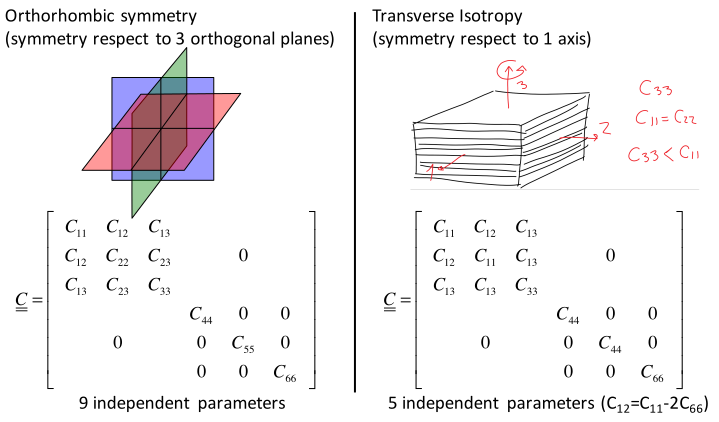
\includegraphics[scale=0.55]{.././Figures/split/4-22.pdf}%
\lthtmlpictureZ
\lthtmlcheckvsize\clearpage}

{\newpage\clearpage
\lthtmlinlinemathA{tex2html_wrap_inline22410}%
$ E_h > E_v$%
\lthtmlindisplaymathZ
\lthtmlcheckvsize\clearpage}

\stepcounter{section}
{\newpage\clearpage
\lthtmlinlinemathA{tex2html_wrap_inline22417}%
$ \varepsilon \gtrsim 0.001$%
\lthtmlindisplaymathZ
\lthtmlcheckvsize\clearpage}

{\newpage\clearpage
\lthtmlinlinemathA{tex2html_wrap_inline22419}%
$ E_{load}$%
\lthtmlindisplaymathZ
\lthtmlcheckvsize\clearpage}

{\newpage\clearpage
\lthtmlinlinemathA{tex2html_wrap_inline22421}%
$ E_{unload}$%
\lthtmlindisplaymathZ
\lthtmlcheckvsize\clearpage}

{\newpage\clearpage
\lthtmlinlinemathA{tex2html_wrap_inline22427}%
$ E_{unload} \sim E_{unload}$%
\lthtmlindisplaymathZ
\lthtmlcheckvsize\clearpage}

{\newpage\clearpage
\lthtmlpictureA{tex2html_wrap22429}%
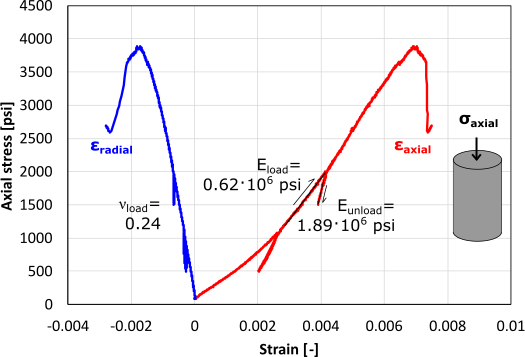
\includegraphics[scale=0.55]{.././Figures/split/LoadingUnloading.pdf}%
\lthtmlpictureZ
\lthtmlcheckvsize\clearpage}

\stepcounter{section}
{\newpage\clearpage
\lthtmlpictureA{tex2html_wrap22439}%
\includegraphics[scale=0.50]{.././Figures/split/5B-18.pdf}%
\lthtmlpictureZ
\lthtmlcheckvsize\clearpage}

{\newpage\clearpage
\lthtmlpictureA{tex2html_wrap22444}%
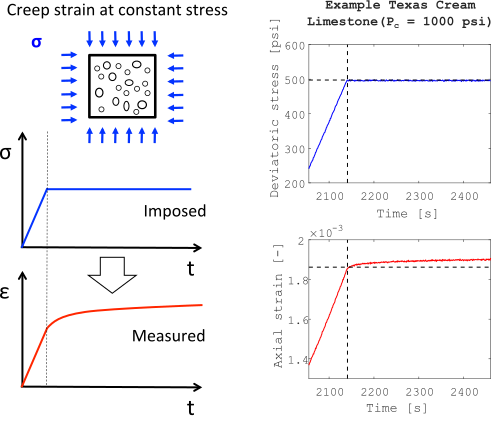
\includegraphics[scale=0.60]{.././Figures/split/5-CreepTXC.pdf}%
\lthtmlpictureZ
\lthtmlcheckvsize\clearpage}

{\newpage\clearpage
\lthtmlpictureA{tex2html_wrap22449}%
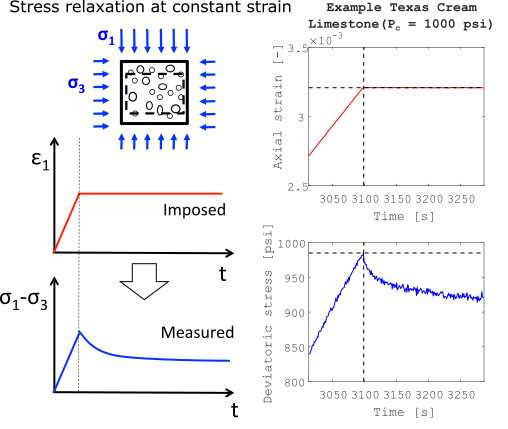
\includegraphics[scale=0.60]{.././Figures/split/5-StressRelaxTXC.pdf}%
\lthtmlpictureZ
\lthtmlcheckvsize\clearpage}

{\newpage\clearpage
\lthtmlpictureA{tex2html_wrap22454}%
\includegraphics[scale=0.45]{.././Figures/split/4-StressRelaxField.PNG}%
\lthtmlpictureZ
\lthtmlcheckvsize\clearpage}

\stepcounter{section}
\stepcounter{subsection}
{\newpage\clearpage
\lthtmlinlinemathA{tex2html_wrap_inline22473}%
$ \uuline{\varepsilon} = \uuline{D} \: \uuline{\sigma}$%
\lthtmlindisplaymathZ
\lthtmlcheckvsize\clearpage}

{\newpage\clearpage
\lthtmlinlinemathA{tex2html_wrap_indisplay22475}%
$\displaystyle \uuline{\sigma} = \uuline{S} - \alpha P_p \uuline{I}$%
\lthtmlindisplaymathZ
\lthtmlcheckvsize\clearpage}

{\newpage\clearpage
\lthtmlinlinemathA{tex2html_wrap_inline22479}%
$ \uuline{I}$%
\lthtmlindisplaymathZ
\lthtmlcheckvsize\clearpage}

{\newpage\clearpage
\lthtmlinlinemathA{tex2html_wrap_indisplay22481}%
$\displaystyle \alpha = 1 - \frac{K_{drained}}{K_{unj}}$%
\lthtmlindisplaymathZ
\lthtmlcheckvsize\clearpage}

{\newpage\clearpage
\lthtmlinlinemathA{tex2html_wrap_inline22483}%
$ K_{drained}$%
\lthtmlindisplaymathZ
\lthtmlcheckvsize\clearpage}

{\newpage\clearpage
\lthtmlinlinemathA{tex2html_wrap_inline22485}%
$ K_{unj}$%
\lthtmlindisplaymathZ
\lthtmlcheckvsize\clearpage}

{\newpage\clearpage
\lthtmlinlinemathA{tex2html_wrap_inline22487}%
$ K_{unj} = K_{m}$%
\lthtmlindisplaymathZ
\lthtmlcheckvsize\clearpage}

{\newpage\clearpage
\lthtmlinlinemathA{tex2html_wrap_inline22489}%
$ \uuline{\alpha}$%
\lthtmlindisplaymathZ
\lthtmlcheckvsize\clearpage}

{\newpage\clearpage
\lthtmlinlinemathA{tex2html_wrap_inline22491}%
$ \alpha \neq 1$%
\lthtmlindisplaymathZ
\lthtmlcheckvsize\clearpage}

\stepcounter{subsection}
{\newpage\clearpage
\lthtmlpictureA{tex2html_wrap22494}%
\includegraphics[scale=0.55]{.././Figures/split/4-23.pdf}%
\lthtmlpictureZ
\lthtmlcheckvsize\clearpage}

{\newpage\clearpage
\lthtmlinlinemathA{tex2html_wrap_inline22499}%
$ \alpha_L$%
\lthtmlindisplaymathZ
\lthtmlcheckvsize\clearpage}

{\newpage\clearpage
\lthtmlinlinemathA{tex2html_wrap_inline22503}%
$ p$%
\lthtmlindisplaymathZ
\lthtmlcheckvsize\clearpage}

{\newpage\clearpage
\lthtmlinlinemathA{tex2html_wrap_indisplay22505}%
$\displaystyle \alpha_L = \left. \cfrac{1}{L} \cfrac{ \mathrm{d} L}{ \mathrm{d} T} \right|_p$%
\lthtmlindisplaymathZ
\lthtmlcheckvsize\clearpage}

{\newpage\clearpage
\lthtmlinlinemathA{tex2html_wrap_inline22507}%
$ \Delta T$%
\lthtmlindisplaymathZ
\lthtmlcheckvsize\clearpage}

{\newpage\clearpage
\lthtmldisplayA{displaymath22509}%
\begin{displaymath}\left\lbrace
\begin{array}{rcl}
\sigma_{11} & = & (\lambda + 2 \mu) \: \varepsilon_{11} + \lambda \: \varepsilon_{22} + \lambda \: \varepsilon_{33} + 3 K \alpha_L \Delta T \\
\sigma_{22} & = & \lambda \: \varepsilon_{11} + (\lambda + 2 \mu) \: \varepsilon_{22} + \lambda \: \varepsilon_{33} + 3 K \alpha_L \Delta T \\
\sigma_{33} & = & \lambda \: \varepsilon_{11} + \lambda \: \varepsilon_{22} + (\lambda + 2 \mu) \: \varepsilon_{33} + 3 K \alpha_L \Delta T \\
\sigma_{12} & = & 2 \mu \: \varepsilon_{12}\\
\sigma_{13} & = & 2 \mu \: \varepsilon_{13}\\
\sigma_{23} & = & 2 \mu \: \varepsilon_{23}\\
\end{array}
\right.\end{displaymath}%
\lthtmldisplayZ
\lthtmlcheckvsize\clearpage}

{\newpage\clearpage
\lthtmlinlinemathA{tex2html_wrap_inline22511}%
$ \sigma_{11}=\sigma_{22}=0$%
\lthtmlindisplaymathZ
\lthtmlcheckvsize\clearpage}

{\newpage\clearpage
\lthtmlinlinemathA{tex2html_wrap_inline22513}%
$ \varepsilon_{11}=\varepsilon_{22} \neq 0$%
\lthtmlindisplaymathZ
\lthtmlcheckvsize\clearpage}

{\newpage\clearpage
\lthtmlinlinemathA{tex2html_wrap_inline22515}%
$ \varepsilon_{33}=0$%
\lthtmlindisplaymathZ
\lthtmlcheckvsize\clearpage}

{\newpage\clearpage
\lthtmlinlinemathA{tex2html_wrap_inline22517}%
$ \Delta T \neq 0$%
\lthtmlindisplaymathZ
\lthtmlcheckvsize\clearpage}

{\newpage\clearpage
\lthtmldisplayA{displaymath22519}%
\begin{displaymath}\left\lbrace
\begin{array}{rcl}
0 & = & (\lambda + 2 \mu) \: \varepsilon_{11} + \lambda \: \varepsilon_{11} + 3 K \alpha_L \Delta T\\
\sigma_{33} & = & \lambda \: \varepsilon_{11} + \lambda \: \varepsilon_{11} + 3 K \alpha_L \Delta T \\
\end{array}
\right.\end{displaymath}%
\lthtmldisplayZ
\lthtmlcheckvsize\clearpage}

{\newpage\clearpage
\lthtmlinlinemathA{tex2html_wrap_indisplay22525}%
$\displaystyle \sigma_{33} = \left( \frac{6-\mu/K}{3+\mu/K} \right) K \alpha_L \Delta T \: \: \blacksquare
$%
\lthtmlindisplaymathZ
\lthtmlcheckvsize\clearpage}

\stepcounter{section}
{\newpage\clearpage
\lthtmlinlinemathA{tex2html_wrap_inline22528}%
$ D = 1.00$%
\lthtmlindisplaymathZ
\lthtmlcheckvsize\clearpage}

{\newpage\clearpage
\lthtmlinlinemathA{tex2html_wrap_inline22530}%
$ L = 2.01$%
\lthtmlindisplaymathZ
\lthtmlcheckvsize\clearpage}

{\newpage\clearpage
\lthtmlinlinemathA{tex2html_wrap_inline22532}%
$ \Delta L$%
\lthtmlindisplaymathZ
\lthtmlcheckvsize\clearpage}

{\newpage\clearpage
\lthtmlinlinemathA{tex2html_wrap_inline22534}%
$ \Delta D$%
\lthtmlindisplaymathZ
\lthtmlcheckvsize\clearpage}

{\newpage\clearpage
\lthtmlinlinemathA{tex2html_wrap_inline22537}%
$ \uline{\sigma} = \uuline{C} \: \uline{\varepsilon}$%
\lthtmlindisplaymathZ
\lthtmlcheckvsize\clearpage}

{\newpage\clearpage
\lthtmlinlinemathA{tex2html_wrap_inline22539}%
$ \sigma_{iso}$%
\lthtmlindisplaymathZ
\lthtmlcheckvsize\clearpage}

{\newpage\clearpage
\lthtmlinlinemathA{tex2html_wrap_inline22541}%
$ \varepsilon_{vol}=\frac{3(1-2\nu)}{E} \sigma_{iso}$%
\lthtmlindisplaymathZ
\lthtmlcheckvsize\clearpage}

{\newpage\clearpage
\lthtmlinlinemathA{tex2html_wrap_inline22543}%
$ \varepsilon_{vol}$%
\lthtmlindisplaymathZ
\lthtmlcheckvsize\clearpage}

{\newpage\clearpage
\lthtmlinlinemathA{tex2html_wrap_inline22545}%
$ E = 4 \times 10^6$%
\lthtmlindisplaymathZ
\lthtmlcheckvsize\clearpage}

{\newpage\clearpage
\lthtmlinlinemathA{tex2html_wrap_inline22547}%
$ \nu = 0.2$%
\lthtmlindisplaymathZ
\lthtmlcheckvsize\clearpage}

{\newpage\clearpage
\lthtmlinlinemathA{tex2html_wrap_inline22549}%
$ \sigma_{iso} =$%
\lthtmlindisplaymathZ
\lthtmlcheckvsize\clearpage}

{\newpage\clearpage
\lthtmlinlinemathA{tex2html_wrap_inline22551}%
$ \times$%
\lthtmlindisplaymathZ
\lthtmlcheckvsize\clearpage}

{\newpage\clearpage
\lthtmlinlinemathA{tex2html_wrap_inline22557}%
$ \sigma_{11} = \cfrac{E(1-\nu)}{(1+\nu)(1-2\nu)} \varepsilon_{11}$%
\lthtmlindisplaymathZ
\lthtmlcheckvsize\clearpage}

{\newpage\clearpage
\lthtmlinlinemathA{tex2html_wrap_inline22561}%
$ 3 \times 3$%
\lthtmlindisplaymathZ
\lthtmlcheckvsize\clearpage}

{\newpage\clearpage
\lthtmlinlinemathA{tex2html_wrap_inline22563}%
$ \phi = 0.35$%
\lthtmlindisplaymathZ
\lthtmlcheckvsize\clearpage}

\stepcounter{section}
\stepcounter{chapter}
\stepcounter{section}
\stepcounter{subsection}
{\newpage\clearpage
\lthtmlpictureA{tex2html_wrap22581}%
\includegraphics[scale=0.65]{.././Figures/split/5A-3.pdf}%
\lthtmlpictureZ
\lthtmlcheckvsize\clearpage}

\stepcounter{subsection}
{\newpage\clearpage
\lthtmlpictureA{tex2html_wrap22587}%
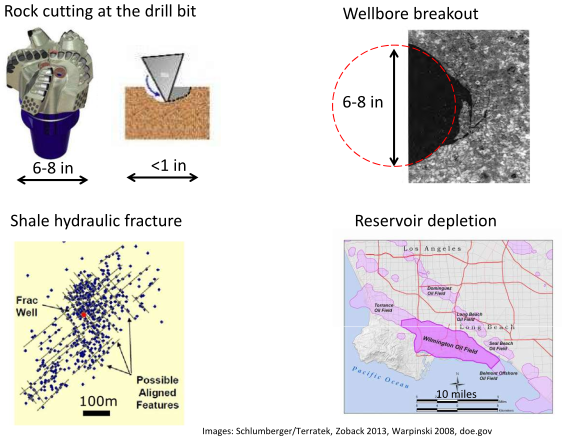
\includegraphics[scale=0.65]{.././Figures/split/5A-4.pdf}%
\lthtmlpictureZ
\lthtmlcheckvsize\clearpage}

\stepcounter{subsection}
{\newpage\clearpage
\lthtmlpictureA{tex2html_wrap22593}%
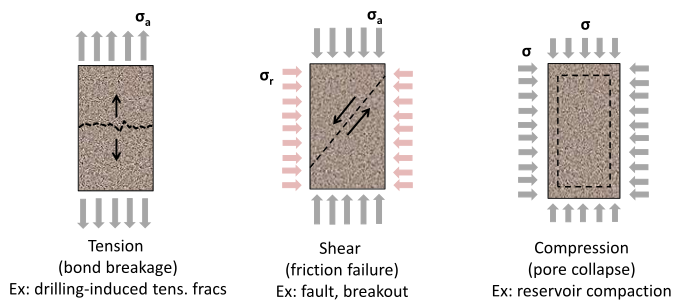
\includegraphics[scale=0.55]{.././Figures/split/5A-5.pdf}%
\lthtmlpictureZ
\lthtmlcheckvsize\clearpage}

\stepcounter{section}
\stepcounter{subsection}
{\newpage\clearpage
\lthtmlpictureA{tex2html_wrap22600}%
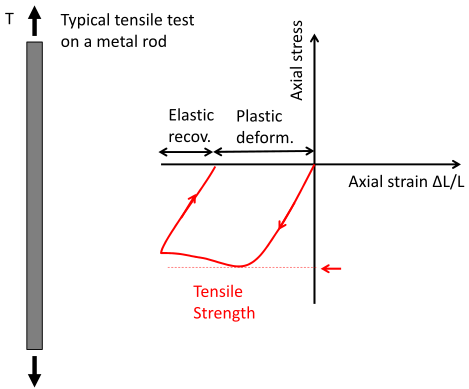
\includegraphics[scale=0.55]{.././Figures/split/5A-6.pdf}%
\lthtmlpictureZ
\lthtmlcheckvsize\clearpage}

{\newpage\clearpage
\lthtmlpictureA{tex2html_wrap22605}%
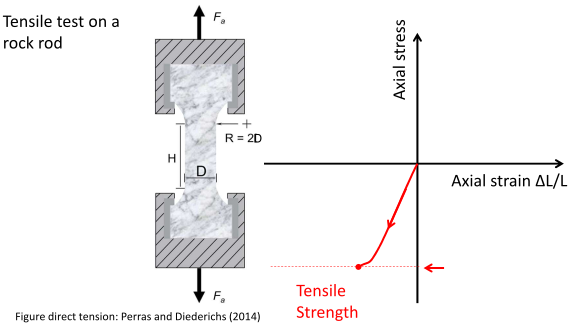
\includegraphics[scale=0.60]{.././Figures/split/5A-7.pdf}%
\lthtmlpictureZ
\lthtmlcheckvsize\clearpage}

\stepcounter{subsection}
{\newpage\clearpage
\lthtmlinlinemathA{tex2html_wrap_indisplay22613}%
$\displaystyle T_S = \frac{P_B}{\pi L R}$%
\lthtmlindisplaymathZ
\lthtmlcheckvsize\clearpage}

{\newpage\clearpage
\lthtmlinlinemathA{tex2html_wrap_inline22615}%
$ P_B$%
\lthtmlindisplaymathZ
\lthtmlcheckvsize\clearpage}

{\newpage\clearpage
\lthtmlinlinemathA{tex2html_wrap_inline22619}%
$ R$%
\lthtmlindisplaymathZ
\lthtmlcheckvsize\clearpage}

{\newpage\clearpage
\lthtmlpictureA{tex2html_wrap22621}%
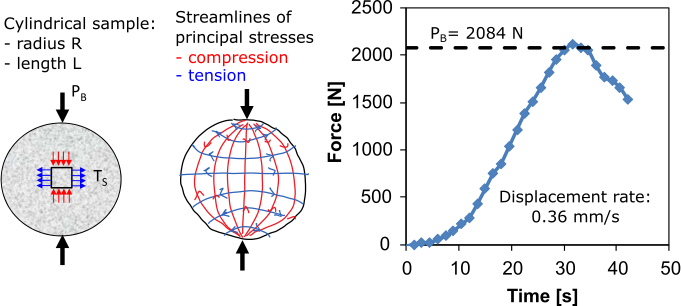
\includegraphics[scale=0.55]{.././Figures/split/4-TensileStrength.pdf}%
\lthtmlpictureZ
\lthtmlcheckvsize\clearpage}

{\newpage\clearpage
\lthtmlinlinemathA{tex2html_wrap_indisplay22626}%
$\displaystyle R = \frac{1}{2}$%
\lthtmlindisplaymathZ
\lthtmlcheckvsize\clearpage}

{\newpage\clearpage
\lthtmlinlinemathA{tex2html_wrap_indisplay22627}%
$\displaystyle = 0.0127$%
\lthtmlindisplaymathZ
\lthtmlcheckvsize\clearpage}

{\newpage\clearpage
\lthtmlinlinemathA{tex2html_wrap_indisplay22629}%
$\displaystyle L = 1$%
\lthtmlindisplaymathZ
\lthtmlcheckvsize\clearpage}

{\newpage\clearpage
\lthtmlinlinemathA{tex2html_wrap_indisplay22630}%
$\displaystyle = 0.0254$%
\lthtmlindisplaymathZ
\lthtmlcheckvsize\clearpage}

{\newpage\clearpage
\lthtmlinlinemathA{tex2html_wrap_indisplay22632}%
$\displaystyle T_S = \frac{2084 \text { N}}{\pi (0.0254 \text{ m}) (0.0127 \text{ m})}
= 2.06 \times 10^6 \text{ Pa} = 2.06 \text{ MPa} \: \: \blacksquare$%
\lthtmlindisplaymathZ
\lthtmlcheckvsize\clearpage}

{\newpage\clearpage
\lthtmlpictureA{tex2html_wrap22634}%
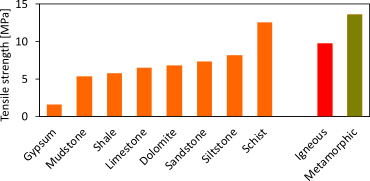
\includegraphics[scale=0.65]{.././Figures/split/4-TensStrengthSummary.pdf}%
\lthtmlpictureZ
\lthtmlcheckvsize\clearpage}

\stepcounter{section}
\stepcounter{subsection}
{\newpage\clearpage
\lthtmlinlinemathA{tex2html_wrap_inline22641}%
$ S_0$%
\lthtmlindisplaymathZ
\lthtmlcheckvsize\clearpage}

{\newpage\clearpage
\lthtmlinlinemathA{tex2html_wrap_inline22643}%
$ F_T$%
\lthtmlindisplaymathZ
\lthtmlcheckvsize\clearpage}

{\newpage\clearpage
\lthtmlinlinemathA{tex2html_wrap_inline22647}%
$ F_N$%
\lthtmlindisplaymathZ
\lthtmlcheckvsize\clearpage}

{\newpage\clearpage
\lthtmlinlinemathA{tex2html_wrap_inline22649}%
$ F_T = \mu F_N$%
\lthtmlindisplaymathZ
\lthtmlcheckvsize\clearpage}

{\newpage\clearpage
\lthtmlinlinemathA{tex2html_wrap_inline22651}%
$ F_N=0$%
\lthtmlindisplaymathZ
\lthtmlcheckvsize\clearpage}

{\newpage\clearpage
\lthtmlinlinemathA{tex2html_wrap_inline22653}%
$ F_T = 0$%
\lthtmlindisplaymathZ
\lthtmlcheckvsize\clearpage}

{\newpage\clearpage
\lthtmlpictureA{tex2html_wrap22659}%
\includegraphics[scale=0.65]{.././Figures/split/5-Friction.pdf}%
\lthtmlpictureZ
\lthtmlcheckvsize\clearpage}

{\newpage\clearpage
\lthtmlinlinemathA{tex2html_wrap_inline22664}%
$ \tau$%
\lthtmlindisplaymathZ
\lthtmlcheckvsize\clearpage}

{\newpage\clearpage
\lthtmlinlinemathA{tex2html_wrap_inline22666}%
$ \sigma_n$%
\lthtmlindisplaymathZ
\lthtmlcheckvsize\clearpage}

{\newpage\clearpage
\lthtmlinlinemathA{tex2html_wrap_inline22668}%
$ \mu_i$%
\lthtmlindisplaymathZ
\lthtmlcheckvsize\clearpage}

{\newpage\clearpage
\lthtmlinlinemathA{tex2html_wrap_inline22670}%
$ \tau = \mu_i \sigma_n$%
\lthtmlindisplaymathZ
\lthtmlcheckvsize\clearpage}

{\newpage\clearpage
\lthtmlpictureA{tex2html_wrap22672}%
\includegraphics[scale=0.50]{.././Figures/split/5A-14.pdf}%
\lthtmlpictureZ
\lthtmlcheckvsize\clearpage}

{\newpage\clearpage
\lthtmlinlinemathA{tex2html_wrap_inline22683}%
$ \sigma_n = 0$%
\lthtmlindisplaymathZ
\lthtmlcheckvsize\clearpage}

{\newpage\clearpage
\lthtmlinlinemathA{tex2html_wrap_inline22685}%
$ \tau = 0$%
\lthtmlindisplaymathZ
\lthtmlcheckvsize\clearpage}

{\newpage\clearpage
\lthtmlinlinemathA{tex2html_wrap_inline22689}%
$ \varphi$%
\lthtmlindisplaymathZ
\lthtmlcheckvsize\clearpage}

{\newpage\clearpage
\lthtmlinlinemathA{tex2html_wrap_inline22691}%
$ \tan (\varphi) = \mu_i$%
\lthtmlindisplaymathZ
\lthtmlcheckvsize\clearpage}

{\newpage\clearpage
\lthtmlinlinemathA{tex2html_wrap_inline22695}%
$ \mu_i=0.5$%
\lthtmlindisplaymathZ
\lthtmlcheckvsize\clearpage}

{\newpage\clearpage
\lthtmlinlinemathA{tex2html_wrap_inline22697}%
$ \varphi \sim 30^{\circ}$%
\lthtmlindisplaymathZ
\lthtmlcheckvsize\clearpage}

\stepcounter{subsection}
{\newpage\clearpage
\lthtmlinlinemathA{tex2html_wrap_inline22700}%
$ \sigma_r = 0$%
\lthtmlindisplaymathZ
\lthtmlcheckvsize\clearpage}

{\newpage\clearpage
\lthtmlpictureA{tex2html_wrap22708}%
\includegraphics[scale=0.60]{.././Figures/split/5A-12.pdf}%
\lthtmlpictureZ
\lthtmlcheckvsize\clearpage}

\stepcounter{subsection}
{\newpage\clearpage
\lthtmlinlinemathA{tex2html_wrap_inline22714}%
$ \sigma_r \neq 0$%
\lthtmlindisplaymathZ
\lthtmlcheckvsize\clearpage}

{\newpage\clearpage
\lthtmlinlinemathA{tex2html_wrap_indisplay22722}%
$\displaystyle \tau = S_0 + \mu_i \sigma_n$%
\lthtmlindisplaymathZ
\lthtmlcheckvsize\clearpage}

{\newpage\clearpage
\lthtmlpictureA{tex2html_wrap22724}%
\includegraphics[scale=0.60]{.././Figures/split/5A-13.pdf}%
\lthtmlpictureZ
\lthtmlcheckvsize\clearpage}

{\newpage\clearpage
\lthtmlinlinemathA{tex2html_wrap_inline22733}%
$ \pi/4 + \varphi/2$%
\lthtmlindisplaymathZ
\lthtmlcheckvsize\clearpage}

{\newpage\clearpage
\lthtmlinlinemathA{tex2html_wrap_inline22737}%
$ \pi/4 + \varphi/2 = 60^{\circ}$%
\lthtmlindisplaymathZ
\lthtmlcheckvsize\clearpage}

{\newpage\clearpage
\lthtmlinlinemathA{tex2html_wrap_inline22741}%
$ \sigma_a / \sigma_r$%
\lthtmlindisplaymathZ
\lthtmlcheckvsize\clearpage}

{\newpage\clearpage
\lthtmlpictureA{tex2html_wrap22743}%
\includegraphics[scale=0.50]{.././Figures/split/5A-15.pdf}%
\lthtmlpictureZ
\lthtmlcheckvsize\clearpage}

{\newpage\clearpage
\lthtmlinlinemathA{tex2html_wrap_inline22747}%
$ \tau / \sigma_n = \mu_i$%
\lthtmlindisplaymathZ
\lthtmlcheckvsize\clearpage}

{\newpage\clearpage
\lthtmlpictureA{tex2html_wrap22749}%
\includegraphics[scale=0.55]{.././Figures/split/AngleFailurePlane.pdf}%
\lthtmlpictureZ
\lthtmlcheckvsize\clearpage}

{\newpage\clearpage
\lthtmlinlinemathA{tex2html_wrap_inline22751}%
$ (\sigma_a,0)$%
\lthtmlindisplaymathZ
\lthtmlcheckvsize\clearpage}

{\newpage\clearpage
\lthtmlinlinemathA{tex2html_wrap_inline22757}%
$ (\sigma_r,0)$%
\lthtmlindisplaymathZ
\lthtmlcheckvsize\clearpage}

{\newpage\clearpage
\lthtmlinlinemathA{tex2html_wrap_inline22763}%
$ (\sigma_n,\tau)$%
\lthtmlindisplaymathZ
\lthtmlcheckvsize\clearpage}

{\newpage\clearpage
\lthtmlinlinemathA{tex2html_wrap_inline22765}%
$ \pi/2 + \varphi$%
\lthtmlindisplaymathZ
\lthtmlcheckvsize\clearpage}

{\newpage\clearpage
\lthtmlinlinemathA{tex2html_wrap_inline22771}%
$ (\pi/2 + \varphi)/2$%
\lthtmlindisplaymathZ
\lthtmlcheckvsize\clearpage}

{\newpage\clearpage
\lthtmlinlinemathA{tex2html_wrap_inline22777}%
$ ^{\circ} = \pi/2$%
\lthtmlindisplaymathZ
\lthtmlcheckvsize\clearpage}

{\newpage\clearpage
\lthtmlinlinemathA{tex2html_wrap_inline22779}%
$ C$%
\lthtmlindisplaymathZ
\lthtmlcheckvsize\clearpage}

{\newpage\clearpage
\lthtmlinlinemathA{tex2html_wrap_indisplay22785}%
$\displaystyle \frac{\sigma_a}{\sigma_r} = \frac{C + R}{C-R} = 
		\frac{C+C \sin \varphi}{C-C \sin \varphi} =
		\frac{1+\sin \varphi}{1-\sin \varphi} =		
 \: \: \blacksquare
$%
\lthtmlindisplaymathZ
\lthtmlcheckvsize\clearpage}

{\newpage\clearpage
\lthtmlinlinemathA{tex2html_wrap_indisplay22787}%
$\displaystyle \sigma_1 = UCS + q \: \sigma_3$%
\lthtmlindisplaymathZ
\lthtmlcheckvsize\clearpage}

{\newpage\clearpage
\lthtmlinlinemathA{tex2html_wrap_inline22793}%
$ q$%
\lthtmlindisplaymathZ
\lthtmlcheckvsize\clearpage}

{\newpage\clearpage
\lthtmlinlinemathA{tex2html_wrap_inline22797}%
$ p'-q$%
\lthtmlindisplaymathZ
\lthtmlcheckvsize\clearpage}

{\newpage\clearpage
\lthtmlinlinemathA{tex2html_wrap_inline22799}%
$ \sigma_m-q$%
\lthtmlindisplaymathZ
\lthtmlcheckvsize\clearpage}

{\newpage\clearpage
\lthtmlinlinemathA{tex2html_wrap_indisplay22801}%
$\displaystyle q = \frac{1 + \sin \varphi}{1 - \sin \varphi}$%
\lthtmlindisplaymathZ
\lthtmlcheckvsize\clearpage}

{\newpage\clearpage
\lthtmlinlinemathA{tex2html_wrap_inline22803}%
$ \varphi ~ 30^{\circ}$%
\lthtmlindisplaymathZ
\lthtmlcheckvsize\clearpage}

{\newpage\clearpage
\lthtmlinlinemathA{tex2html_wrap_inline22805}%
$ q = 3$%
\lthtmlindisplaymathZ
\lthtmlcheckvsize\clearpage}

{\newpage\clearpage
\lthtmlinlinemathA{tex2html_wrap_indisplay22809}%
$\displaystyle \mu_i = \frac{q-1}{2 \sqrt{q}}$%
\lthtmlindisplaymathZ
\lthtmlcheckvsize\clearpage}

{\newpage\clearpage
\lthtmlinlinemathA{tex2html_wrap_indisplay22813}%
$\displaystyle UCS = 2 S_0 \left( \frac{1 + \sin \varphi}{1 - \sin \varphi} \right)^{1/2}
= 2 S_0 \sqrt{q}$%
\lthtmlindisplaymathZ
\lthtmlcheckvsize\clearpage}

{\newpage\clearpage
\lthtmlpictureA{tex2html_wrap22815}%
\includegraphics[scale=0.65]{.././Figures/split/5A-16.pdf}%
\lthtmlpictureZ
\lthtmlcheckvsize\clearpage}

{\newpage\clearpage
\lthtmlpictureA{tex2html_wrap22820}%
\includegraphics[scale=0.85]{.././Figures/split/4-ShearStrengthSummary.pdf}%
\lthtmlpictureZ
\lthtmlcheckvsize\clearpage}

\stepcounter{subsection}
{\newpage\clearpage
\lthtmlinlinemathA{tex2html_wrap_inline22826}%
$ (S_1,S_2,S_3)$%
\lthtmlindisplaymathZ
\lthtmlcheckvsize\clearpage}

{\newpage\clearpage
\lthtmlinlinemathA{tex2html_wrap_inline22828}%
$ (\sigma_1,\sigma_2,\sigma_3)$%
\lthtmlindisplaymathZ
\lthtmlcheckvsize\clearpage}

{\newpage\clearpage
\lthtmlinlinemathA{tex2html_wrap_inline22830}%
$ P_c$%
\lthtmlindisplaymathZ
\lthtmlcheckvsize\clearpage}

{\newpage\clearpage
\lthtmlinlinemathA{tex2html_wrap_inline22832}%
$ \sigma_D$%
\lthtmlindisplaymathZ
\lthtmlcheckvsize\clearpage}

{\newpage\clearpage
\lthtmlinlinemathA{tex2html_wrap_inline22838}%
$ P_c = cst$%
\lthtmlindisplaymathZ
\lthtmlcheckvsize\clearpage}

{\newpage\clearpage
\lthtmlinlinemathA{tex2html_wrap_inline22842}%
$ P_p < P_c$%
\lthtmlindisplaymathZ
\lthtmlcheckvsize\clearpage}

{\newpage\clearpage
\lthtmlinlinemathA{tex2html_wrap_inline22844}%
$ P_p = cst$%
\lthtmlindisplaymathZ
\lthtmlcheckvsize\clearpage}

{\newpage\clearpage
\lthtmlinlinemathA{tex2html_wrap_inline22848}%
$ \sigma_D =S_1 - S_3$%
\lthtmlindisplaymathZ
\lthtmlcheckvsize\clearpage}

{\newpage\clearpage
\lthtmlinlinemathA{tex2html_wrap_inline22854}%
$ S_3 = P_c$%
\lthtmlindisplaymathZ
\lthtmlcheckvsize\clearpage}

{\newpage\clearpage
\lthtmlinlinemathA{tex2html_wrap_inline22856}%
$ S_2=S_3$%
\lthtmlindisplaymathZ
\lthtmlcheckvsize\clearpage}

{\newpage\clearpage
\lthtmlinlinemathA{tex2html_wrap_inline22858}%
$ S_1 - S_3=\sigma_1-\sigma_3$%
\lthtmlindisplaymathZ
\lthtmlcheckvsize\clearpage}

{\newpage\clearpage
\lthtmlinlinemathA{tex2html_wrap_inline22860}%
$ d \varepsilon_a / dt = cst$%
\lthtmlindisplaymathZ
\lthtmlcheckvsize\clearpage}

{\newpage\clearpage
\lthtmlinlinemathA{tex2html_wrap_inline22894}%
$ \sigma_1 = (S_1 - P_p)$%
\lthtmlindisplaymathZ
\lthtmlcheckvsize\clearpage}

{\newpage\clearpage
\lthtmlinlinemathA{tex2html_wrap_inline22896}%
$ \sigma_3 = (S_3 - P_p)$%
\lthtmlindisplaymathZ
\lthtmlcheckvsize\clearpage}

{\newpage\clearpage
\lthtmlinlinemathA{tex2html_wrap_indisplay22906}%
$\displaystyle \varphi = \arctan \left( \frac{q-1}{2\sqrt{q}} \right)$%
\lthtmlindisplaymathZ
\lthtmlcheckvsize\clearpage}

{\newpage\clearpage
\lthtmlinlinemathA{tex2html_wrap_inline22918}%
$ S_3 \leqslant 80$%
\lthtmlindisplaymathZ
\lthtmlcheckvsize\clearpage}

{\newpage\clearpage
\lthtmlinlinemathA{tex2html_wrap_inline22920}%
$ S_1 \sim 80$%
\lthtmlindisplaymathZ
\lthtmlcheckvsize\clearpage}

{\newpage\clearpage
\lthtmlinlinemathA{tex2html_wrap_indisplay22922}%
$\displaystyle UCS = 80$%
\lthtmlindisplaymathZ
\lthtmlcheckvsize\clearpage}

{\newpage\clearpage
\lthtmlinlinemathA{tex2html_wrap_indisplay22923}%
$\displaystyle $%
\lthtmlindisplaymathZ
\lthtmlcheckvsize\clearpage}

{\newpage\clearpage
\lthtmlinlinemathA{tex2html_wrap_indisplay22927}%
$\displaystyle q = \frac{\Delta \sigma_1}{\Delta \sigma_3} = 
       \frac{520 \text{ MPa}}{110 \text{ MPa}} = 4.73
$%
\lthtmlindisplaymathZ
\lthtmlcheckvsize\clearpage}

{\newpage\clearpage
\lthtmlinlinemathA{tex2html_wrap_indisplay22929}%
$\displaystyle S_0 = \frac{UCS}{2 \sqrt{q}} = \frac{80 \text{MPa}}{2 \sqrt{4.73}} = 18.4 \text{MPa} $%
\lthtmlindisplaymathZ
\lthtmlcheckvsize\clearpage}

{\newpage\clearpage
\lthtmlinlinemathA{tex2html_wrap_indisplay22931}%
$\displaystyle \varphi = \arctan \left( \frac{q-1}{2\sqrt{q}} \right) 
        = \arctan \left( \frac{4.73-1}{2\sqrt{4.73}} \right) = 40.6^{\circ} 
$%
\lthtmlindisplaymathZ
\lthtmlcheckvsize\clearpage}

{\newpage\clearpage
\lthtmlinlinemathA{tex2html_wrap_indisplay22933}%
$\displaystyle \mu_i = \tan (\varphi) = \tan (40.6^{\circ}) = 0.86 
\: \: \blacksquare
$%
\lthtmlindisplaymathZ
\lthtmlcheckvsize\clearpage}

{\newpage\clearpage
\lthtmlinlinemathA{tex2html_wrap_inline22935}%
$ \varepsilon_v = \varepsilon_a + 2\varepsilon_r$%
\lthtmlindisplaymathZ
\lthtmlcheckvsize\clearpage}

{\newpage\clearpage
\lthtmlinlinemathA{tex2html_wrap_inline22937}%
$ d \varepsilon_v/dt<0$%
\lthtmlindisplaymathZ
\lthtmlcheckvsize\clearpage}

{\newpage\clearpage
\lthtmlpictureA{tex2html_wrap22939}%
\includegraphics[scale=0.65]{.././Figures/split/Triaxial-Darley.pdf}%
\lthtmlpictureZ
\lthtmlcheckvsize\clearpage}

\stepcounter{section}
{\newpage\clearpage
\lthtmlpictureA{tex2html_wrap22947}%
\includegraphics[scale=0.65]{.././Figures/split/5A-21.pdf}%
\lthtmlpictureZ
\lthtmlcheckvsize\clearpage}

\stepcounter{section}
{\newpage\clearpage
\lthtmlinlinemathA{tex2html_wrap_inline22961}%
$ \tau = S_0 + \mu_i \sigma_n$%
\lthtmlindisplaymathZ
\lthtmlcheckvsize\clearpage}

{\newpage\clearpage
\lthtmlpictureA{tex2html_wrap22963}%
\includegraphics[scale=0.55]{.././Figures/split/5B-YieldLocus.pdf}%
\lthtmlpictureZ
\lthtmlcheckvsize\clearpage}

\stepcounter{section}
{\newpage\clearpage
\lthtmlpictureA{tex2html_wrap22971}%
\includegraphics[scale=0.75]{.././Figures/split/5-StrengthAnisotropy.pdf}%
\lthtmlpictureZ
\lthtmlcheckvsize\clearpage}

\stepcounter{section}
{\newpage\clearpage
\lthtmlpictureA{tex2html_wrap22977}%
\includegraphics[scale=0.65]{.././Figures/split/5B-9.pdf}%
\lthtmlpictureZ
\lthtmlcheckvsize\clearpage}

{\newpage\clearpage
\lthtmlinlinemathA{tex2html_wrap_inline22982}%
$ E/\nu$%
\lthtmlindisplaymathZ
\lthtmlcheckvsize\clearpage}

{\newpage\clearpage
\lthtmlpictureA{tex2html_wrap22988}%
\includegraphics[scale=0.65]{.././Figures/split/5B-10.pdf}%
\lthtmlpictureZ
\lthtmlcheckvsize\clearpage}

{\newpage\clearpage
\lthtmlinlinemathA{tex2html_wrap_inline22993}%
$ \sigma_d = (\sigma_1 - \sigma_3)$%
\lthtmlindisplaymathZ
\lthtmlcheckvsize\clearpage}

{\newpage\clearpage
\lthtmlinlinemathA{tex2html_wrap_inline22995}%
$ \uuline{\varepsilon}{}_p$%
\lthtmlindisplaymathZ
\lthtmlcheckvsize\clearpage}

{\newpage\clearpage
\lthtmlinlinemathA{tex2html_wrap_inline22997}%
$ \uuline{C}{}_p$%
\lthtmlindisplaymathZ
\lthtmlcheckvsize\clearpage}

{\newpage\clearpage
\lthtmlinlinemathA{tex2html_wrap_indisplay22999}%
$\displaystyle \Delta \uuline{\sigma} = \uuline{C}{}_p \Delta \uuline{\varepsilon}{}_p$%
\lthtmlindisplaymathZ
\lthtmlcheckvsize\clearpage}

{\newpage\clearpage
\lthtmlpictureA{tex2html_wrap23001}%
\includegraphics[scale=0.60]{.././Figures/split/5B-11.pdf}%
\lthtmlpictureZ
\lthtmlcheckvsize\clearpage}

\stepcounter{section}
{\newpage\clearpage
\lthtmlpictureA{tex2html_wrap23007}%
\includegraphics[scale=0.65]{.././Figures/split/5B-12.pdf}%
\lthtmlpictureZ
\lthtmlcheckvsize\clearpage}

{\newpage\clearpage
\lthtmlpictureA{tex2html_wrap23012}%
\includegraphics[scale=0.60]{.././Figures/split/5B-13.pdf}%
\lthtmlpictureZ
\lthtmlcheckvsize\clearpage}

{\newpage\clearpage
\lthtmlpictureA{tex2html_wrap23017}%
\includegraphics[scale=0.55]{.././Figures/split/5B-14.pdf}%
\lthtmlpictureZ
\lthtmlcheckvsize\clearpage}

\stepcounter{section}
{\newpage\clearpage
\lthtmlinlinemathA{tex2html_wrap_inline23027}%
$ S_1 - S_3$%
\lthtmlindisplaymathZ
\lthtmlcheckvsize\clearpage}

{\newpage\clearpage
\lthtmlinlinemathA{tex2html_wrap_inline23053}%
$ \varphi = f(q)$%
\lthtmlindisplaymathZ
\lthtmlcheckvsize\clearpage}

{\newpage\clearpage
\lthtmlinlinemathA{tex2html_wrap_inline23059}%
$ Sig_D$%
\lthtmlindisplaymathZ
\lthtmlcheckvsize\clearpage}

{\newpage\clearpage
\lthtmlinlinemathA{tex2html_wrap_inline23063}%
$ E_x$%
\lthtmlindisplaymathZ
\lthtmlcheckvsize\clearpage}

{\newpage\clearpage
\lthtmlinlinemathA{tex2html_wrap_inline23065}%
$ E_y$%
\lthtmlindisplaymathZ
\lthtmlcheckvsize\clearpage}

{\newpage\clearpage
\lthtmlinlinemathA{tex2html_wrap_inline23067}%
$ q=5.3$%
\lthtmlindisplaymathZ
\lthtmlcheckvsize\clearpage}

{\newpage\clearpage
\lthtmlinlinemathA{tex2html_wrap_inline23073}%
$ S_1=S_3 \rightarrow S_1-S_3=0$%
\lthtmlindisplaymathZ
\lthtmlcheckvsize\clearpage}

{\newpage\clearpage
\lthtmlinlinemathA{tex2html_wrap_inline23134}%
$ S_o$%
\lthtmlindisplaymathZ
\lthtmlcheckvsize\clearpage}

\stepcounter{section}
\stepcounter{chapter}
\stepcounter{section}
{\newpage\clearpage
\lthtmlpictureA{tex2html_wrap23145}%
\includegraphics[scale=0.60]{.././Figures/split/6-2.pdf}%
\lthtmlpictureZ
\lthtmlcheckvsize\clearpage}

\stepcounter{section}
{\newpage\clearpage
\lthtmlpictureA{tex2html_wrap23155}%
\includegraphics[scale=0.60]{.././Figures/split/6-8.pdf}%
\lthtmlpictureZ
\lthtmlcheckvsize\clearpage}

\stepcounter{subsection}
{\newpage\clearpage
\lthtmlinlinemathA{tex2html_wrap_inline23165}%
$ dip$%
\lthtmlindisplaymathZ
\lthtmlcheckvsize\clearpage}

{\newpage\clearpage
\lthtmlpictureA{tex2html_wrap23191}%
\includegraphics[scale=0.65]{.././Figures/split/6-5.pdf}%
\lthtmlpictureZ
\lthtmlcheckvsize\clearpage}

\stepcounter{subsection}
\stepcounter{subsection}
{\newpage\clearpage
\lthtmlpictureA{tex2html_wrap23224}%
\includegraphics[scale=0.55]{.././Figures/split/6-7.pdf}%
\lthtmlpictureZ
\lthtmlcheckvsize\clearpage}

\stepcounter{section}
\stepcounter{subsection}
{\newpage\clearpage
\lthtmlinlinemathA{tex2html_wrap_indisplay23245}%
$\displaystyle \sigma_1 = q \: \sigma_3$%
\lthtmlindisplaymathZ
\lthtmlcheckvsize\clearpage}

{\newpage\clearpage
\lthtmlinlinemathA{tex2html_wrap_indisplay23247}%
$\displaystyle q = \left( \sqrt{\mu^2 +1} + \mu \right) ^2 = \frac{1+\sin \: \varphi}{1-\sin \: \varphi}$%
\lthtmlindisplaymathZ
\lthtmlcheckvsize\clearpage}

{\newpage\clearpage
\lthtmlinlinemathA{tex2html_wrap_inline23251}%
$ \sigma_1/\sigma_3 \sim $%
\lthtmlindisplaymathZ
\lthtmlcheckvsize\clearpage}

{\newpage\clearpage
\lthtmlpictureA{tex2html_wrap23253}%
\includegraphics[scale=0.65]{.././Figures/split/6-20.pdf}%
\lthtmlpictureZ
\lthtmlcheckvsize\clearpage}

{\newpage\clearpage
\lthtmlinlinemathA{tex2html_wrap_inline23267}%
$ \pi/4 + \phi/2$%
\lthtmlindisplaymathZ
\lthtmlcheckvsize\clearpage}

{\newpage\clearpage
\lthtmlinlinemathA{tex2html_wrap_inline23269}%
$ \sim 30 ^{\circ}$%
\lthtmlindisplaymathZ
\lthtmlcheckvsize\clearpage}

{\newpage\clearpage
\lthtmlinlinemathA{tex2html_wrap_inline23271}%
$ \sim 60 ^{\circ}$%
\lthtmlindisplaymathZ
\lthtmlcheckvsize\clearpage}

{\newpage\clearpage
\lthtmlinlinemathA{tex2html_wrap_inline23273}%
$ 45 ^{\circ}$%
\lthtmlindisplaymathZ
\lthtmlcheckvsize\clearpage}

{\newpage\clearpage
\lthtmlinlinemathA{tex2html_wrap_inline23275}%
$ 67.5 ^{\circ}$%
\lthtmlindisplaymathZ
\lthtmlcheckvsize\clearpage}

{\newpage\clearpage
\lthtmlinlinemathA{tex2html_wrap_inline23277}%
$ 50 ^{\circ}$%
\lthtmlindisplaymathZ
\lthtmlcheckvsize\clearpage}

{\newpage\clearpage
\lthtmlinlinemathA{tex2html_wrap_inline23279}%
$ 70 ^{\circ}$%
\lthtmlindisplaymathZ
\lthtmlcheckvsize\clearpage}

{\newpage\clearpage
\lthtmlinlinemathA{tex2html_wrap_inline23297}%
$ \sigma_1 / \sigma_3 > q$%
\lthtmlindisplaymathZ
\lthtmlcheckvsize\clearpage}

{\newpage\clearpage
\lthtmlinlinemathA{tex2html_wrap_inline23299}%
$ \sigma_1 / \sigma_3 < q$%
\lthtmlindisplaymathZ
\lthtmlcheckvsize\clearpage}

\stepcounter{subsection}
{\newpage\clearpage
\lthtmldisplayA{displaymath23302}%
\begin{displaymath}\left\lbrace
\begin{array}{l}
S_1 = S_v \\
S_2 = S_{Hmax} \\
S_3 = S_{hmin} \\
\end{array}
\right.\end{displaymath}%
\lthtmldisplayZ
\lthtmlcheckvsize\clearpage}

{\newpage\clearpage
\lthtmlinlinemathA{tex2html_wrap_inline23304}%
$ S_1 > S_2 > S_3$%
\lthtmlindisplaymathZ
\lthtmlcheckvsize\clearpage}

{\newpage\clearpage
\lthtmlpictureA{tex2html_wrap23316}%
\includegraphics[scale=0.50]{.././Figures/split/6-12.pdf}%
\lthtmlpictureZ
\lthtmlcheckvsize\clearpage}

{\newpage\clearpage
\lthtmlinlinemathA{tex2html_wrap_inline23321}%
$ S_1 \neq S_2 \neq S_3$%
\lthtmlindisplaymathZ
\lthtmlcheckvsize\clearpage}

{\newpage\clearpage
\lthtmlpictureA{tex2html_wrap23323}%
\includegraphics[scale=0.55]{.././Figures/split/6-13.pdf}%
\lthtmlpictureZ
\lthtmlcheckvsize\clearpage}

\stepcounter{subsection}
{\newpage\clearpage
\lthtmldisplayA{displaymath23329}%
\begin{displaymath}\left\lbrace
\begin{array}{l}
S_1 = S_{Hmax} \\
S_2 = S_{hmin} \\
S_3 = S_v \\
\end{array}
\right.\end{displaymath}%
\lthtmldisplayZ
\lthtmlcheckvsize\clearpage}

{\newpage\clearpage
\lthtmlinlinemathA{tex2html_wrap_inline23331}%
$ (\pi/4 + \varphi/2)$%
\lthtmlindisplaymathZ
\lthtmlcheckvsize\clearpage}

{\newpage\clearpage
\lthtmlinlinemathA{tex2html_wrap_inline23335}%
$ S_{v}$%
\lthtmlindisplaymathZ
\lthtmlcheckvsize\clearpage}

{\newpage\clearpage
\lthtmlpictureA{tex2html_wrap23341}%
\includegraphics[scale=0.55]{.././Figures/split/6-14.pdf}%
\lthtmlpictureZ
\lthtmlcheckvsize\clearpage}

{\newpage\clearpage
\lthtmlpictureA{tex2html_wrap23346}%
\includegraphics[scale=0.55]{.././Figures/split/6-15.pdf}%
\lthtmlpictureZ
\lthtmlcheckvsize\clearpage}

\stepcounter{subsection}
{\newpage\clearpage
\lthtmldisplayA{displaymath23352}%
\begin{displaymath}\left\lbrace
\begin{array}{l}
S_1 = S_{Hmax} \\
S_2 = S_v \\
S_3 = S_{hmin} \\
\end{array}
\right.\end{displaymath}%
\lthtmldisplayZ
\lthtmlcheckvsize\clearpage}

{\newpage\clearpage
\lthtmlpictureA{tex2html_wrap23360}%
\includegraphics[scale=0.65]{.././Figures/split/6-16.pdf}%
\lthtmlpictureZ
\lthtmlcheckvsize\clearpage}

\stepcounter{subsection}
{\newpage\clearpage
\lthtmlpictureA{tex2html_wrap23413}%
\includegraphics[scale=0.65]{.././Figures/split/6-18.pdf}%
\lthtmlpictureZ
\lthtmlcheckvsize\clearpage}

\stepcounter{subsection}
{\newpage\clearpage
\lthtmlpictureA{tex2html_wrap23439}%
\includegraphics[scale=0.50]{.././Figures/split/6-IdealFaultOrientationGC.pdf}%
\lthtmlpictureZ
\lthtmlcheckvsize\clearpage}

{\newpage\clearpage
\lthtmlpictureA{tex2html_wrap23470}%
\includegraphics[scale=0.75]{.././Figures/split/6-IdealFracP1.pdf}%
\lthtmlpictureZ
\lthtmlcheckvsize\clearpage}

{\newpage\clearpage
\lthtmlinlinemathA{tex2html_wrap_inline23476}%
$ \phi_{HF} = 030^{\circ}$%
\lthtmlindisplaymathZ
\lthtmlcheckvsize\clearpage}

{\newpage\clearpage
\lthtmlinlinemathA{tex2html_wrap_inline23478}%
$ \delta_{HF} = 90^{\circ}$%
\lthtmlindisplaymathZ
\lthtmlcheckvsize\clearpage}

{\newpage\clearpage
\lthtmlinlinemathA{tex2html_wrap_indisplay23482}%
$\displaystyle \beta = 45^{\circ} + \varphi / 2 =  45^{\circ} + 30^{\circ} / 2 = 60^{\circ} $%
\lthtmlindisplaymathZ
\lthtmlcheckvsize\clearpage}

{\newpage\clearpage
\lthtmlinlinemathA{tex2html_wrap_inline23490}%
$ \phi_{F1} = \phi_{F2} = 030^{\circ}$%
\lthtmlindisplaymathZ
\lthtmlcheckvsize\clearpage}

{\newpage\clearpage
\lthtmlinlinemathA{tex2html_wrap_inline23492}%
$ \delta_{F1} = 60^{\circ}$%
\lthtmlindisplaymathZ
\lthtmlcheckvsize\clearpage}

{\newpage\clearpage
\lthtmlpictureA{tex2html_wrap23520}%
\includegraphics[scale=0.75]{.././Figures/split/6-IdealFracP2.pdf}%
\lthtmlpictureZ
\lthtmlcheckvsize\clearpage}

{\newpage\clearpage
\lthtmlinlinemathA{tex2html_wrap_inline23526}%
$ \phi_{HF} = 010^{\circ}$%
\lthtmlindisplaymathZ
\lthtmlcheckvsize\clearpage}

{\newpage\clearpage
\lthtmlinlinemathA{tex2html_wrap_indisplay23532}%
$\displaystyle \beta = 45^{\circ} + \varphi / 2 =  45^{\circ} + 40^{\circ} / 2 = 65^{\circ} $%
\lthtmlindisplaymathZ
\lthtmlcheckvsize\clearpage}

{\newpage\clearpage
\lthtmlinlinemathA{tex2html_wrap_inline23540}%
$ \phi_{F1} = 345^{\circ}$%
\lthtmlindisplaymathZ
\lthtmlcheckvsize\clearpage}

{\newpage\clearpage
\lthtmlinlinemathA{tex2html_wrap_inline23542}%
$ \phi_{F2} =  035^{\circ}$%
\lthtmlindisplaymathZ
\lthtmlcheckvsize\clearpage}

{\newpage\clearpage
\lthtmlinlinemathA{tex2html_wrap_inline23544}%
$ \delta_{F1} = \delta_{F2} = 90^{\circ}$%
\lthtmlindisplaymathZ
\lthtmlcheckvsize\clearpage}

\stepcounter{section}
\stepcounter{subsection}
{\newpage\clearpage
\lthtmlinlinemathA{tex2html_wrap_inline23560}%
$ _1$%
\lthtmlindisplaymathZ
\lthtmlcheckvsize\clearpage}

{\newpage\clearpage
\lthtmlinlinemathA{tex2html_wrap_inline23576}%
$ \beta_1$%
\lthtmlindisplaymathZ
\lthtmlcheckvsize\clearpage}

{\newpage\clearpage
\lthtmlinlinemathA{tex2html_wrap_inline23582}%
$ \sigma_{v}$%
\lthtmlindisplaymathZ
\lthtmlcheckvsize\clearpage}

{\newpage\clearpage
\lthtmlinlinemathA{tex2html_wrap_inline23596}%
$ \beta_2$%
\lthtmlindisplaymathZ
\lthtmlcheckvsize\clearpage}

{\newpage\clearpage
\lthtmlinlinemathA{tex2html_wrap_inline23600}%
$ _3$%
\lthtmlindisplaymathZ
\lthtmlcheckvsize\clearpage}

{\newpage\clearpage
\lthtmlinlinemathA{tex2html_wrap_inline23616}%
$ \beta_3$%
\lthtmlindisplaymathZ
\lthtmlcheckvsize\clearpage}

{\newpage\clearpage
\lthtmlpictureA{tex2html_wrap23620}%
\includegraphics[scale=0.75]{.././Figures/split/6-3DMohrCircle.pdf}%
\lthtmlpictureZ
\lthtmlcheckvsize\clearpage}

{\newpage\clearpage
\lthtmlinlinemathA{tex2html_wrap_inline23629}%
$ \varphi = 30^{\circ}$%
\lthtmlindisplaymathZ
\lthtmlcheckvsize\clearpage}

{\newpage\clearpage
\lthtmlpictureA{tex2html_wrap23647}%
\includegraphics[scale=0.65]{.././Figures/split/6-3DMohrCircleP1.pdf}%
\lthtmlpictureZ
\lthtmlcheckvsize\clearpage}

{\newpage\clearpage
\lthtmlinlinemathA{tex2html_wrap_inline23649}%
$ \sigma_v =$%
\lthtmlindisplaymathZ
\lthtmlcheckvsize\clearpage}

{\newpage\clearpage
\lthtmlinlinemathA{tex2html_wrap_inline23651}%
$ \sigma_{Hmax} =$%
\lthtmlindisplaymathZ
\lthtmlcheckvsize\clearpage}

{\newpage\clearpage
\lthtmlinlinemathA{tex2html_wrap_inline23653}%
$ \sigma_{hmin} =$%
\lthtmlindisplaymathZ
\lthtmlcheckvsize\clearpage}

{\newpage\clearpage
\lthtmlinlinemathA{tex2html_wrap_indisplay23659}%
$\displaystyle \sigma_n = \left( \frac{13 \text{ MPa} + 3.8 \text{ MPa}}{2} \right) + \left( \frac{13 \text{ MPa} - 3.8 \text{ MPa}}{2} \right) \cos(2 \cdot 60^{\circ}) = 6.1 \text{ MPa}
$%
\lthtmlindisplaymathZ
\lthtmlcheckvsize\clearpage}

{\newpage\clearpage
\lthtmlinlinemathA{tex2html_wrap_indisplay23661}%
$\displaystyle \tau = \left( \frac{13 \text{ MPa} - 3.8 \text{ MPa}}{2} \right) \sin(2 \cdot 60^{\circ}) = 4.0 \text{ MPa} 
	\: \: \blacksquare
$%
\lthtmlindisplaymathZ
\lthtmlcheckvsize\clearpage}

{\newpage\clearpage
\lthtmlpictureA{tex2html_wrap23677}%
\includegraphics[scale=0.65]{.././Figures/split/6-3DMohrCircleP2.pdf}%
\lthtmlpictureZ
\lthtmlcheckvsize\clearpage}

{\newpage\clearpage
\lthtmlinlinemathA{tex2html_wrap_indisplay23689}%
$\displaystyle \sigma_n = \left( \frac{30 \text{ MPa} + 10 \text{ MPa}}{2} \right) + \left( \frac{30 \text{ MPa} - 10 \text{ MPa}}{2} \right) \cos(2 \cdot 30^{\circ}) = 25 \text{ MPa}
$%
\lthtmlindisplaymathZ
\lthtmlcheckvsize\clearpage}

{\newpage\clearpage
\lthtmlinlinemathA{tex2html_wrap_indisplay23691}%
$\displaystyle \tau = \left( \frac{30 \text{ MPa} - 10 \text{ MPa}}{2} \right) \sin(2 \cdot 30^{\circ}) = 8.7 \text{ MPa} 
	\: \: \blacksquare
$%
\lthtmlindisplaymathZ
\lthtmlcheckvsize\clearpage}

\stepcounter{subsection}
{\newpage\clearpage
\lthtmlinlinemathA{tex2html_wrap_inline23696}%
$ (strike,dip)$%
\lthtmlindisplaymathZ
\lthtmlcheckvsize\clearpage}

{\newpage\clearpage
\lthtmlinlinemathA{tex2html_wrap_inline23698}%
$ \uuline{S}{}_P$%
\lthtmlindisplaymathZ
\lthtmlcheckvsize\clearpage}

{\newpage\clearpage
\lthtmlinlinemathA{tex2html_wrap_inline23720}%
$ \uuline{S}{}_G$%
\lthtmlindisplaymathZ
\lthtmlcheckvsize\clearpage}

{\newpage\clearpage
\lthtmlpictureA{tex2html_wrap23722}%
\includegraphics[scale=0.55]{.././Figures/split/6-32.pdf}%
\lthtmlpictureZ
\lthtmlcheckvsize\clearpage}

{\newpage\clearpage
\lthtmlinlinemathA{tex2html_wrap_inline23727}%
$ R_{PG}$%
\lthtmlindisplaymathZ
\lthtmlcheckvsize\clearpage}

{\newpage\clearpage
\lthtmlpictureA{tex2html_wrap23741}%
\includegraphics[scale=0.65]{.././Figures/split/6-33.pdf}%
\lthtmlpictureZ
\lthtmlcheckvsize\clearpage}

{\newpage\clearpage
\lthtmldisplayA{displaymath23746}%
\begin{displaymath}R_{PG}
=
\left[
\begin{array}{ccc}
\cos \alpha \cos \beta & \sin \alpha \cos \beta  & -\sin \beta \\
\cos \alpha \sin \beta \sin \gamma - \sin \alpha \cos \gamma  & \sin \alpha \sin \beta \sin \gamma + \cos \alpha \cos \gamma  & \cos \beta \sin \gamma \\
\cos \alpha \sin \beta \cos \gamma + \sin \alpha \sin \gamma  & \sin \alpha \sin \beta \cos \gamma - \cos \alpha \sin \gamma  & \cos \beta \cos \gamma
\end{array}
\right]\end{displaymath}%
\lthtmldisplayZ
\lthtmlcheckvsize\clearpage}

{\newpage\clearpage
\lthtmlinlinemathA{tex2html_wrap_inline23777}%
$ 90^{\circ}$%
\lthtmlindisplaymathZ
\lthtmlcheckvsize\clearpage}

{\newpage\clearpage
\lthtmlinlinemathA{tex2html_wrap_inline23779}%
$ 0^{\circ}$%
\lthtmlindisplaymathZ
\lthtmlcheckvsize\clearpage}

{\newpage\clearpage
\lthtmlinlinemathA{tex2html_wrap_indisplay23819}%
$\displaystyle \uuline{S}_P = R_{PG} \uuline{S}{}_G R_{PG}^T$%
\lthtmlindisplaymathZ
\lthtmlcheckvsize\clearpage}

{\newpage\clearpage
\lthtmlinlinemathA{tex2html_wrap_indisplay23821}%
$\displaystyle \uuline{S}_G = R_{PG}^T \uuline{S}{}_P R_{PG}$%
\lthtmlindisplaymathZ
\lthtmlcheckvsize\clearpage}

{\newpage\clearpage
\lthtmlinlinemathA{tex2html_wrap_inline23827}%
$ S_1 = 30$%
\lthtmlindisplaymathZ
\lthtmlcheckvsize\clearpage}

{\newpage\clearpage
\lthtmlinlinemathA{tex2html_wrap_inline23829}%
$ S_2 = 25$%
\lthtmlindisplaymathZ
\lthtmlcheckvsize\clearpage}

{\newpage\clearpage
\lthtmlinlinemathA{tex2html_wrap_inline23831}%
$ S_3 = 20$%
\lthtmlindisplaymathZ
\lthtmlcheckvsize\clearpage}

{\newpage\clearpage
\lthtmldisplayA{displaymath23837}%
\begin{displaymath}\uuline{S}{}_P
=
\left[
\begin{array}{ccc}
30 & 0  & 0 \\
0  & 25 & 0 \\
0  &  0 & 20
\end{array}
\right]\end{displaymath}%
\lthtmldisplayZ
\lthtmlcheckvsize\clearpage}

{\newpage\clearpage
\lthtmlinlinemathA{tex2html_wrap_inline23841}%
$ \alpha = 0^{\circ}$%
\lthtmlindisplaymathZ
\lthtmlcheckvsize\clearpage}

{\newpage\clearpage
\lthtmlinlinemathA{tex2html_wrap_inline23843}%
$ \beta = 90^{\circ}$%
\lthtmlindisplaymathZ
\lthtmlcheckvsize\clearpage}

{\newpage\clearpage
\lthtmlinlinemathA{tex2html_wrap_inline23845}%
$ \gamma = 0^{\circ}$%
\lthtmlindisplaymathZ
\lthtmlcheckvsize\clearpage}

{\newpage\clearpage
\lthtmldisplayA{displaymath23847}%
\begin{displaymath}R_{PG}
=
\left[
\begin{array}{ccc}
0  & 0  & -1 \\
0  & 1  & 0 \\
1  & 0  & 0
\end{array}
\right]\end{displaymath}%
\lthtmldisplayZ
\lthtmlcheckvsize\clearpage}

{\newpage\clearpage
\lthtmldisplayA{displaymath23849}%
\begin{displaymath}\uuline{S}{}_G
=
\left[
\begin{array}{ccc}
0  & 0  & -1 \\
0  & 1  & 0 \\
1  & 0  & 0
\end{array}
\right]^T
\:
\left[
\begin{array}{ccc}
30 & 0  & 0 \\
0  & 25 & 0 \\
0  &  0 & 20
\end{array}
\right]
\:
\left[
\begin{array}{ccc}
0  & 0  & -1 \\
0  & 1  & 0 \\
1  & 0  & 0
\end{array}
\right]
=
\left[
\begin{array}{ccc}
20 & 0  & 0 \\
0  & 25 & 0 \\
0  &  0 & 30
\end{array}
\right]
\: \: \blacksquare\end{displaymath}%
\lthtmldisplayZ
\lthtmlcheckvsize\clearpage}

{\newpage\clearpage
\lthtmlinlinemathA{tex2html_wrap_inline23871}%
$ \beta = 0^{\circ}$%
\lthtmlindisplaymathZ
\lthtmlcheckvsize\clearpage}

{\newpage\clearpage
\lthtmlinlinemathA{tex2html_wrap_inline23873}%
$ \gamma = 90^{\circ}$%
\lthtmlindisplaymathZ
\lthtmlcheckvsize\clearpage}

{\newpage\clearpage
\lthtmldisplayA{displaymath23875}%
\begin{displaymath}R_{PG}
=
\left[
\begin{array}{ccc}
1  & 0  & 0 \\
0  & 0  & 1 \\
0  & -1 & 0
\end{array}
\right]\end{displaymath}%
\lthtmldisplayZ
\lthtmlcheckvsize\clearpage}

{\newpage\clearpage
\lthtmldisplayA{displaymath23877}%
\begin{displaymath}\uuline{S}{}_G
=
\left[
\begin{array}{ccc}
1  & 0  & 0 \\
0  & 0  & 1 \\
0  & -1 & 0
\end{array}
\right]^T
\:
\left[
\begin{array}{ccc}
30 & 0  & 0 \\
0  & 25 & 0 \\
0  &  0 & 20
\end{array}
\right]
\:
\left[
\begin{array}{ccc}
1  & 0  & 0 \\
0  & 0  & 1 \\
0  & -1 & 0
\end{array}
\right]
=
\left[
\begin{array}{ccc}
30 & 0  & 0 \\
0  & 20 & 0 \\
0  &  0 & 25
\end{array}
\right]
\: \: \blacksquare\end{displaymath}%
\lthtmldisplayZ
\lthtmlcheckvsize\clearpage}

{\newpage\clearpage
\lthtmlinlinemathA{tex2html_wrap_inline23897}%
$ \alpha = 90^{\circ}$%
\lthtmlindisplaymathZ
\lthtmlcheckvsize\clearpage}

{\newpage\clearpage
\lthtmldisplayA{displaymath23903}%
\begin{displaymath}R_{PG}
=
\left[
\begin{array}{ccc}
0  & 1  & 0 \\
-1 & 0  & 0 \\
0  & 0  & 1
\end{array}
\right]\end{displaymath}%
\lthtmldisplayZ
\lthtmlcheckvsize\clearpage}

{\newpage\clearpage
\lthtmldisplayA{displaymath23905}%
\begin{displaymath}\uuline{S}{}_G
=
\left[
\begin{array}{ccc}
0  & 1  & 0 \\
-1 & 0  & 0 \\
0  & 0  & 1
\end{array}
\right]^T
\:
\left[
\begin{array}{ccc}
30 & 0  & 0 \\
0  & 25 & 0 \\
0  &  0 & 20
\end{array}
\right]
\:
\left[
\begin{array}{ccc}
0  & 1  & 0 \\
-1 & 0  & 0 \\
0  & 0  & 1
\end{array}
\right]
=
\left[
\begin{array}{ccc}
25 & 0  & 0 \\
0  & 30 & 0 \\
0  &  0 & 20
\end{array}
\right]
\: \: \blacksquare\end{displaymath}%
\lthtmldisplayZ
\lthtmlcheckvsize\clearpage}

{\newpage\clearpage
\lthtmlinlinemathA{tex2html_wrap_inline23909}%
$ S_1 = 60$%
\lthtmlindisplaymathZ
\lthtmlcheckvsize\clearpage}

{\newpage\clearpage
\lthtmlinlinemathA{tex2html_wrap_inline23911}%
$ S_2 = 40$%
\lthtmlindisplaymathZ
\lthtmlcheckvsize\clearpage}

{\newpage\clearpage
\lthtmlinlinemathA{tex2html_wrap_inline23913}%
$ S_3 = 35$%
\lthtmlindisplaymathZ
\lthtmlcheckvsize\clearpage}

{\newpage\clearpage
\lthtmldisplayA{displaymath23921}%
\begin{displaymath}\uuline{S}{}_P
=
\left[
\begin{array}{ccc}
60 & 0  & 0 \\
0  & 40 & 0 \\
0  &  0 & 35
\end{array}
\right]\end{displaymath}%
\lthtmldisplayZ
\lthtmlcheckvsize\clearpage}

{\newpage\clearpage
\lthtmlinlinemathA{tex2html_wrap_inline23927}%
$ \alpha = 135^{\circ}$%
\lthtmlindisplaymathZ
\lthtmlcheckvsize\clearpage}

{\newpage\clearpage
\lthtmldisplayA{displaymath23933}%
\begin{displaymath}R_{PG}
=
\left[
\begin{array}{ccc}
-0.707  & 0.707  & 0 \\
0  & 0  & 1 \\
0.707  & 0.707 & 0
\end{array}
\right]\end{displaymath}%
\lthtmldisplayZ
\lthtmlcheckvsize\clearpage}

{\newpage\clearpage
\lthtmldisplayA{displaymath23935}%
\begin{displaymath}\uuline{S}{}_G
=
\left[
\begin{array}{ccc}
-0.707  & 0.707  & 0 \\
0  & 0  & 1 \\
0.707  & 0.707 & 0
\end{array}
\right]^T
\:
\left[
\begin{array}{ccc}
60 & 0  & 0 \\
0  & 40 & 0 \\
0  &  0 & 35
\end{array}
\right]
\:
\left[
\begin{array}{ccc}
-0.707  & 0.707  & 0 \\
0  & 0  & 1 \\
0.707  & 0.707 & 0
\end{array}
\right]
=
\left[
\begin{array}{ccc}
47.5  & -12.5  & 0 \\
-12.5  &  47.5  & 0 \\
0    &  0     & 40
\end{array}
\right]
\: \: \blacksquare\end{displaymath}%
\lthtmldisplayZ
\lthtmlcheckvsize\clearpage}

{\newpage\clearpage
\lthtmlinlinemathA{tex2html_wrap_inline23937}%
$ n_d$%
\lthtmlindisplaymathZ
\lthtmlcheckvsize\clearpage}

{\newpage\clearpage
\lthtmlinlinemathA{tex2html_wrap_inline23939}%
$ n_s$%
\lthtmlindisplaymathZ
\lthtmlcheckvsize\clearpage}

{\newpage\clearpage
\lthtmlinlinemathA{tex2html_wrap_inline23941}%
$ n_n$%
\lthtmlindisplaymathZ
\lthtmlcheckvsize\clearpage}

{\newpage\clearpage
\lthtmlinlinemathA{tex2html_wrap_inline23943}%
$ strike$%
\lthtmlindisplaymathZ
\lthtmlcheckvsize\clearpage}

{\newpage\clearpage
\lthtmlpictureA{tex2html_wrap23947}%
\includegraphics[scale=0.60]{.././Figures/split/6-39.pdf}%
\lthtmlpictureZ
\lthtmlcheckvsize\clearpage}

{\newpage\clearpage
\lthtmlinlinemathA{tex2html_wrap_inline23956}%
$ \uline{n}_d$%
\lthtmlindisplaymathZ
\lthtmlcheckvsize\clearpage}

{\newpage\clearpage
\lthtmlinlinemathA{tex2html_wrap_inline23958}%
$ \uline{n}_s$%
\lthtmlindisplaymathZ
\lthtmlcheckvsize\clearpage}

{\newpage\clearpage
\lthtmlinlinemathA{tex2html_wrap_inline23960}%
$ \uline{n}_n$%
\lthtmlindisplaymathZ
\lthtmlcheckvsize\clearpage}

{\newpage\clearpage
\lthtmlinlinemathA{tex2html_wrap_indisplay23962}%
$\displaystyle \uline{t} = \uuline{S}{}_G \uline{n}_n$%
\lthtmlindisplaymathZ
\lthtmlcheckvsize\clearpage}

{\newpage\clearpage
\lthtmlinlinemathA{tex2html_wrap_inline23964}%
$ S_n$%
\lthtmlindisplaymathZ
\lthtmlcheckvsize\clearpage}

{\newpage\clearpage
\lthtmlinlinemathA{tex2html_wrap_indisplay23968}%
$\displaystyle S_n = \uline{t} \cdot \uline{n}_n$%
\lthtmlindisplaymathZ
\lthtmlcheckvsize\clearpage}

{\newpage\clearpage
\lthtmlinlinemathA{tex2html_wrap_inline23970}%
$ \sigma_n = S_n - P_p $%
\lthtmlindisplaymathZ
\lthtmlcheckvsize\clearpage}

{\newpage\clearpage
\lthtmldisplayA{displaymath23976}%
\begin{displaymath}\left\lbrace
\begin{array}{l}
\tau_d = \uline{t} \cdot \uline{n}_d \\
\tau_s = \uline{t} \cdot \uline{n}_s
\end{array}
\right.\end{displaymath}%
\lthtmldisplayZ
\lthtmlcheckvsize\clearpage}

{\newpage\clearpage
\lthtmlinlinemathA{tex2html_wrap_inline23980}%
$ \tau = \sqrt{\tau_d^2 + \tau_s^2}$%
\lthtmlindisplaymathZ
\lthtmlcheckvsize\clearpage}

{\newpage\clearpage
\lthtmlinlinemathA{tex2html_wrap_indisplay23982}%
$\displaystyle \sigma_n = \uline{t} \cdot \uline{n}_n - P_p$%
\lthtmlindisplaymathZ
\lthtmlcheckvsize\clearpage}

{\newpage\clearpage
\lthtmlinlinemathA{tex2html_wrap_indisplay23984}%
$\displaystyle \tau^2 = ||\uline{t}||^2 - ||\uline{t} \cdot \uline{n}_n||^2$%
\lthtmlindisplaymathZ
\lthtmlcheckvsize\clearpage}

{\newpage\clearpage
\lthtmlinlinemathA{tex2html_wrap_inline23986}%
$ rake$%
\lthtmlindisplaymathZ
\lthtmlcheckvsize\clearpage}

{\newpage\clearpage
\lthtmlinlinemathA{tex2html_wrap_inline23988}%
$ \uline{\tau}_d + \uline{\tau}_s$%
\lthtmlindisplaymathZ
\lthtmlcheckvsize\clearpage}

{\newpage\clearpage
\lthtmlinlinemathA{tex2html_wrap_indisplay23992}%
$\displaystyle rake = \arctan \left( \frac{\tau_d}{\tau_s} \right)$%
\lthtmlindisplaymathZ
\lthtmlcheckvsize\clearpage}

{\newpage\clearpage
\lthtmlinlinemathA{tex2html_wrap_inline23994}%
$ t$%
\lthtmlindisplaymathZ
\lthtmlcheckvsize\clearpage}

{\newpage\clearpage
\lthtmlinlinemathA{tex2html_wrap_inline23998}%
$ \tau_d$%
\lthtmlindisplaymathZ
\lthtmlcheckvsize\clearpage}

{\newpage\clearpage
\lthtmlinlinemathA{tex2html_wrap_inline24000}%
$ \tau_s$%
\lthtmlindisplaymathZ
\lthtmlcheckvsize\clearpage}

{\newpage\clearpage
\lthtmlinlinemathA{tex2html_wrap_inline24008}%
$ S_v = 23$%
\lthtmlindisplaymathZ
\lthtmlcheckvsize\clearpage}

{\newpage\clearpage
\lthtmlinlinemathA{tex2html_wrap_inline24010}%
$ S_{Hmax} = 15$%
\lthtmlindisplaymathZ
\lthtmlcheckvsize\clearpage}

{\newpage\clearpage
\lthtmlinlinemathA{tex2html_wrap_inline24012}%
$ S_{hmin} = 13.8$%
\lthtmlindisplaymathZ
\lthtmlcheckvsize\clearpage}

{\newpage\clearpage
\lthtmldisplayA{displaymath24020}%
\begin{displaymath}\uuline{S}{}_P
=
\left[
\begin{array}{ccc}
23 & 0  & 0 \\
0  & 15 & 0 \\
0  &  0 & 13.8
\end{array}
\right]\end{displaymath}%
\lthtmldisplayZ
\lthtmlcheckvsize\clearpage}

{\newpage\clearpage
\lthtmldisplayA{displaymath24034}%
\begin{displaymath}R_{PG}
=
\left[
\begin{array}{ccc}
0  & 0  & -1 \\
-1  & 0  & 0 \\
0  & 1 & 0
\end{array}
\right]\end{displaymath}%
\lthtmldisplayZ
\lthtmlcheckvsize\clearpage}

{\newpage\clearpage
\lthtmldisplayA{displaymath24036}%
\begin{displaymath}\uuline{S}{}_G
=
\left[
\begin{array}{ccc}
15 & 0  & 0 \\
0  & 13.8 & 0 \\
0  &  0 & 23
\end{array}
\right]\end{displaymath}%
\lthtmldisplayZ
\lthtmlcheckvsize\clearpage}

{\newpage\clearpage
\lthtmldisplayA{displaymath24038}%
\begin{displaymath}\uline{n}{}_n
=
\left[
\begin{array}{c}
0 \\
0.867 \\
-0.5
\end{array}
\right]\end{displaymath}%
\lthtmldisplayZ
\lthtmlcheckvsize\clearpage}

{\newpage\clearpage
\lthtmlinlinemathA{tex2html_wrap_inline24040}%
$ \uline{t}= [0,11.95,-11.50]$%
\lthtmlindisplaymathZ
\lthtmlcheckvsize\clearpage}

{\newpage\clearpage
\lthtmlinlinemathA{tex2html_wrap_inline24042}%
$ S_n = 16.1$%
\lthtmlindisplaymathZ
\lthtmlcheckvsize\clearpage}

{\newpage\clearpage
\lthtmlinlinemathA{tex2html_wrap_inline24044}%
$ \tau_d = -3.98$%
\lthtmlindisplaymathZ
\lthtmlcheckvsize\clearpage}

{\newpage\clearpage
\lthtmlinlinemathA{tex2html_wrap_inline24046}%
$ \tau_s = 0$%
\lthtmlindisplaymathZ
\lthtmlcheckvsize\clearpage}

{\newpage\clearpage
\lthtmlinlinemathA{tex2html_wrap_inline24050}%
$ ^{\circ} \: \: \blacksquare $%
\lthtmlindisplaymathZ
\lthtmlcheckvsize\clearpage}

{\newpage\clearpage
\lthtmlinlinemathA{tex2html_wrap_inline24066}%
$ S_v = 30$%
\lthtmlindisplaymathZ
\lthtmlcheckvsize\clearpage}

{\newpage\clearpage
\lthtmlinlinemathA{tex2html_wrap_inline24068}%
$ S_{Hmax} = 45$%
\lthtmlindisplaymathZ
\lthtmlcheckvsize\clearpage}

{\newpage\clearpage
\lthtmlinlinemathA{tex2html_wrap_inline24070}%
$ S_{hmin} = 25$%
\lthtmlindisplaymathZ
\lthtmlcheckvsize\clearpage}

{\newpage\clearpage
\lthtmldisplayA{displaymath24078}%
\begin{displaymath}\uuline{S}{}_P
=
\left[
\begin{array}{ccc}
45 & 0  & 0 \\
0  & 30 & 0 \\
0  &  0 & 25
\end{array}
\right] \text{ MPa}\end{displaymath}%
\lthtmldisplayZ
\lthtmlcheckvsize\clearpage}

{\newpage\clearpage
\lthtmlinlinemathA{tex2html_wrap_inline24086}%
$ \alpha = 120^{\circ}$%
\lthtmlindisplaymathZ
\lthtmlcheckvsize\clearpage}

{\newpage\clearpage
\lthtmldisplayA{displaymath24092}%
\begin{displaymath}R_{PG}
=
\left[
\begin{array}{ccc}
-0.5  & 0.866  & 0 \\
0  & 0  & 1 \\
0.866  & 0.5 & 0
\end{array}
\right]\end{displaymath}%
\lthtmldisplayZ
\lthtmlcheckvsize\clearpage}

{\newpage\clearpage
\lthtmldisplayA{displaymath24094}%
\begin{displaymath}\uuline{S}{}_G
=
\left[
\begin{array}{ccc}
30 & -8.66  & 0 \\
-8.66  & 40 & 0 \\
0  &  0 & 30
\end{array}
\right] \text{ MPa}\end{displaymath}%
\lthtmldisplayZ
\lthtmlcheckvsize\clearpage}

{\newpage\clearpage
\lthtmldisplayA{displaymath24096}%
\begin{displaymath}\uline{n}{}_n
=
\left[
\begin{array}{c}
-0.866 \\
0.5 \\
0
\end{array}
\right]\end{displaymath}%
\lthtmldisplayZ
\lthtmlcheckvsize\clearpage}

{\newpage\clearpage
\lthtmlinlinemathA{tex2html_wrap_inline24098}%
$ \uline{t}= [-30.31,27.5,0]$%
\lthtmlindisplaymathZ
\lthtmlcheckvsize\clearpage}

{\newpage\clearpage
\lthtmlinlinemathA{tex2html_wrap_inline24100}%
$ S_n = 40$%
\lthtmlindisplaymathZ
\lthtmlcheckvsize\clearpage}

{\newpage\clearpage
\lthtmlinlinemathA{tex2html_wrap_inline24102}%
$ \tau_d = 0$%
\lthtmlindisplaymathZ
\lthtmlcheckvsize\clearpage}

{\newpage\clearpage
\lthtmlinlinemathA{tex2html_wrap_inline24104}%
$ \tau_s = 8.66$%
\lthtmlindisplaymathZ
\lthtmlcheckvsize\clearpage}

{\newpage\clearpage
\lthtmlinlinemathA{tex2html_wrap_inline24126}%
$ S_v = 5000$%
\lthtmlindisplaymathZ
\lthtmlcheckvsize\clearpage}

{\newpage\clearpage
\lthtmlinlinemathA{tex2html_wrap_inline24128}%
$ S_{Hmax} = 4000$%
\lthtmlindisplaymathZ
\lthtmlcheckvsize\clearpage}

{\newpage\clearpage
\lthtmlinlinemathA{tex2html_wrap_inline24130}%
$ S_{hmin} = 3000$%
\lthtmlindisplaymathZ
\lthtmlcheckvsize\clearpage}

{\newpage\clearpage
\lthtmldisplayA{displaymath24138}%
\begin{displaymath}\uuline{S}{}_P
=
\left[
\begin{array}{ccc}
5000 & 0  & 0 \\
0  & 4000 & 0 \\
0  &  0 & 3000
\end{array}
\right] \text{ psi}\end{displaymath}%
\lthtmldisplayZ
\lthtmlcheckvsize\clearpage}

{\newpage\clearpage
\lthtmldisplayA{displaymath24154}%
\begin{displaymath}\uuline{S}{}_G
=
\left[
\begin{array}{ccc}
4000 & 0  & 0 \\
0  & 3000 & 0 \\
0  &  0 & 5000
\end{array}
\right] \text{ psi}\end{displaymath}%
\lthtmldisplayZ
\lthtmlcheckvsize\clearpage}

{\newpage\clearpage
\lthtmldisplayA{displaymath24160}%
\begin{displaymath}\uline{n}{}_{n}
=
\left[
\begin{array}{c}
-0.612 \\
0.612 \\
-0.5
\end{array}
\right]\end{displaymath}%
\lthtmldisplayZ
\lthtmlcheckvsize\clearpage}

{\newpage\clearpage
\lthtmlinlinemathA{tex2html_wrap_inline24162}%
$ \uline{t}= [-2450,1840,-2500]$%
\lthtmlindisplaymathZ
\lthtmlcheckvsize\clearpage}

{\newpage\clearpage
\lthtmlinlinemathA{tex2html_wrap_inline24164}%
$ S_n = 3870$%
\lthtmlindisplaymathZ
\lthtmlcheckvsize\clearpage}

{\newpage\clearpage
\lthtmlinlinemathA{tex2html_wrap_inline24166}%
$ \tau_d = -649$%
\lthtmlindisplaymathZ
\lthtmlcheckvsize\clearpage}

{\newpage\clearpage
\lthtmlinlinemathA{tex2html_wrap_inline24168}%
$ \tau_s = -433$%
\lthtmlindisplaymathZ
\lthtmlcheckvsize\clearpage}

{\newpage\clearpage
\lthtmldisplayA{displaymath24178}%
\begin{displaymath}\uline{n}{}_{n}
=
\left[
\begin{array}{c}
0.612 \\
-0.612 \\
-0.5
\end{array}
\right]\end{displaymath}%
\lthtmldisplayZ
\lthtmlcheckvsize\clearpage}

{\newpage\clearpage
\lthtmlinlinemathA{tex2html_wrap_inline24180}%
$ \uline{t}= [2450,-1840,-2500]$%
\lthtmlindisplaymathZ
\lthtmlcheckvsize\clearpage}

{\newpage\clearpage
\lthtmlinlinemathA{tex2html_wrap_inline24208}%
$ S_v = 1000$%
\lthtmlindisplaymathZ
\lthtmlcheckvsize\clearpage}

{\newpage\clearpage
\lthtmlinlinemathA{tex2html_wrap_inline24210}%
$ S_{Hmax} = 2400$%
\lthtmlindisplaymathZ
\lthtmlcheckvsize\clearpage}

{\newpage\clearpage
\lthtmlinlinemathA{tex2html_wrap_inline24212}%
$ S_{hmin} = 1200$%
\lthtmlindisplaymathZ
\lthtmlcheckvsize\clearpage}

{\newpage\clearpage
\lthtmlinlinemathA{tex2html_wrap_inline24218}%
$ P_p = 440$%
\lthtmlindisplaymathZ
\lthtmlcheckvsize\clearpage}

{\newpage\clearpage
\lthtmldisplayA{displaymath24222}%
\begin{displaymath}\uuline{S}{}_P
=
\left[
\begin{array}{ccc}
2400 & 0  & 0 \\
0  & 1200 & 0 \\
0  &  0 & 1000
\end{array}
\right] \text{ psi}\end{displaymath}%
\lthtmldisplayZ
\lthtmlcheckvsize\clearpage}

{\newpage\clearpage
\lthtmlinlinemathA{tex2html_wrap_inline24232}%
$ \alpha = 150^{\circ}$%
\lthtmlindisplaymathZ
\lthtmlcheckvsize\clearpage}

{\newpage\clearpage
\lthtmldisplayA{displaymath24238}%
\begin{displaymath}R_{PG}
=
\left[
\begin{array}{ccc}
-0.866  & 0.5  & 0 \\
-0.5  & -0.866  & 0 \\
0  & 0 & 1
\end{array}
\right]\end{displaymath}%
\lthtmldisplayZ
\lthtmlcheckvsize\clearpage}

{\newpage\clearpage
\lthtmldisplayA{displaymath24240}%
\begin{displaymath}\uuline{S}{}_G
=
\left[
\begin{array}{ccc}
2100 & -520  & 0 \\
-520  & 1500 & 0 \\
0  &  0 & 1000
\end{array}
\right] \text{ psi}\end{displaymath}%
\lthtmldisplayZ
\lthtmlcheckvsize\clearpage}

{\newpage\clearpage
\lthtmldisplayA{displaymath24242}%
\begin{displaymath}\uline{n}{}_n
=
\left[
\begin{array}{c}
-0.814 \\
-0.470 \\
-0.342
\end{array}
\right]\end{displaymath}%
\lthtmldisplayZ
\lthtmlcheckvsize\clearpage}

{\newpage\clearpage
\lthtmlinlinemathA{tex2html_wrap_inline24244}%
$ \uline{t}= [-1465,-281,-342]$%
\lthtmlindisplaymathZ
\lthtmlcheckvsize\clearpage}

{\newpage\clearpage
\lthtmlinlinemathA{tex2html_wrap_inline24246}%
$ S_n = 1441$%
\lthtmlindisplaymathZ
\lthtmlcheckvsize\clearpage}

{\newpage\clearpage
\lthtmlinlinemathA{tex2html_wrap_inline24248}%
$ \sigma_n = 1001$%
\lthtmlindisplaymathZ
\lthtmlcheckvsize\clearpage}

{\newpage\clearpage
\lthtmlinlinemathA{tex2html_wrap_inline24250}%
$ \tau_d = 160$%
\lthtmlindisplaymathZ
\lthtmlcheckvsize\clearpage}

{\newpage\clearpage
\lthtmlinlinemathA{tex2html_wrap_inline24252}%
$ \tau_s = 488$%
\lthtmlindisplaymathZ
\lthtmlcheckvsize\clearpage}

{\newpage\clearpage
\lthtmlinlinemathA{tex2html_wrap_inline24254}%
$ \tau = 514$%
\lthtmlindisplaymathZ
\lthtmlcheckvsize\clearpage}

{\newpage\clearpage
\lthtmlinlinemathA{tex2html_wrap_inline24260}%
$ \tau / \sigma_n = 0.51  \: \: \blacksquare$%
\lthtmlindisplaymathZ
\lthtmlcheckvsize\clearpage}

\stepcounter{section}
\stepcounter{subsection}
{\newpage\clearpage
\lthtmlinlinemathA{tex2html_wrap_inline24272}%
$ \mu \sim$%
\lthtmlindisplaymathZ
\lthtmlcheckvsize\clearpage}

{\newpage\clearpage
\lthtmlinlinemathA{tex2html_wrap_inline24278}%
$ k_{frac} = f(\sigma_n)$%
\lthtmlindisplaymathZ
\lthtmlcheckvsize\clearpage}

{\newpage\clearpage
\lthtmlinlinemathA{tex2html_wrap_inline24280}%
$ k_{frac} = f(\sigma_n,\tau)$%
\lthtmlindisplaymathZ
\lthtmlcheckvsize\clearpage}

\stepcounter{subsection}
{\newpage\clearpage
\lthtmlpictureA{tex2html_wrap24293}%
\includegraphics[scale=0.55]{.././Figures/split/6-21.pdf}%
\lthtmlpictureZ
\lthtmlcheckvsize\clearpage}

{\newpage\clearpage
\lthtmlpictureA{tex2html_wrap24302}%
\includegraphics[scale=0.75]{.././Figures/split/InSituStresses-ElastoPlastic.pdf}%
\lthtmlpictureZ
\lthtmlcheckvsize\clearpage}

{\newpage\clearpage
\lthtmlinlinemathA{tex2html_wrap_inline24317}%
$ q=[1+\sin(\varphi)]/[1-\sin(\varphi)]$%
\lthtmlindisplaymathZ
\lthtmlcheckvsize\clearpage}

{\newpage\clearpage
\lthtmlinlinemathA{tex2html_wrap_inline24321}%
$ \sigma_{v}/q$%
\lthtmlindisplaymathZ
\lthtmlcheckvsize\clearpage}

{\newpage\clearpage
\lthtmlinlinemathA{tex2html_wrap_inline24325}%
$ q \: \sigma_{hmin}$%
\lthtmlindisplaymathZ
\lthtmlcheckvsize\clearpage}

{\newpage\clearpage
\lthtmlinlinemathA{tex2html_wrap_inline24329}%
$ q \: \sigma_{v}$%
\lthtmlindisplaymathZ
\lthtmlcheckvsize\clearpage}

{\newpage\clearpage
\lthtmlinlinemathA{tex2html_wrap_inline24344}%
$ \lambda_p=0.82$%
\lthtmlindisplaymathZ
\lthtmlcheckvsize\clearpage}

{\newpage\clearpage
\lthtmlinlinemathA{tex2html_wrap_indisplay24353}%
$\displaystyle S_v = 1$%
\lthtmlindisplaymathZ
\lthtmlcheckvsize\clearpage}

{\newpage\clearpage
\lthtmlinlinemathA{tex2html_wrap_indisplay24355}%
$\displaystyle = 2000$%
\lthtmlindisplaymathZ
\lthtmlcheckvsize\clearpage}

{\newpage\clearpage
\lthtmlinlinemathA{tex2html_wrap_indisplay24360}%
$\displaystyle P_p = \lambda_p S_v = 0.82 \times 2000$%
\lthtmlindisplaymathZ
\lthtmlcheckvsize\clearpage}

{\newpage\clearpage
\lthtmlinlinemathA{tex2html_wrap_indisplay24361}%
$\displaystyle = 1640$%
\lthtmlindisplaymathZ
\lthtmlcheckvsize\clearpage}

{\newpage\clearpage
\lthtmlinlinemathA{tex2html_wrap_indisplay24364}%
$\displaystyle \sigma_v = S_v - P_p = 2000$%
\lthtmlindisplaymathZ
\lthtmlcheckvsize\clearpage}

{\newpage\clearpage
\lthtmlinlinemathA{tex2html_wrap_indisplay24365}%
$\displaystyle - 1640$%
\lthtmlindisplaymathZ
\lthtmlcheckvsize\clearpage}

{\newpage\clearpage
\lthtmlinlinemathA{tex2html_wrap_indisplay24366}%
$\displaystyle = 360$%
\lthtmlindisplaymathZ
\lthtmlcheckvsize\clearpage}

{\newpage\clearpage
\lthtmlinlinemathA{tex2html_wrap_indisplay24368}%
$\displaystyle \sigma_{Hmax} = q \: \sigma_v = \frac{1+\sin 30^{\circ}}{1-\sin 30^{\circ}} 360$%
\lthtmlindisplaymathZ
\lthtmlcheckvsize\clearpage}

{\newpage\clearpage
\lthtmlinlinemathA{tex2html_wrap_indisplay24369}%
$\displaystyle = 1080$%
\lthtmlindisplaymathZ
\lthtmlcheckvsize\clearpage}

{\newpage\clearpage
\lthtmlinlinemathA{tex2html_wrap_indisplay24371}%
$\displaystyle S_{Hmax} = \sigma_{Hmax} + P_p = 1080$%
\lthtmlindisplaymathZ
\lthtmlcheckvsize\clearpage}

{\newpage\clearpage
\lthtmlinlinemathA{tex2html_wrap_indisplay24372}%
$\displaystyle + 1640$%
\lthtmlindisplaymathZ
\lthtmlcheckvsize\clearpage}

{\newpage\clearpage
\lthtmlinlinemathA{tex2html_wrap_indisplay24373}%
$\displaystyle = 2720$%
\lthtmlindisplaymathZ
\lthtmlcheckvsize\clearpage}

{\newpage\clearpage
\lthtmlinlinemathA{tex2html_wrap_indisplay24374}%
$\displaystyle \: \: \blacksquare $%
\lthtmlindisplaymathZ
\lthtmlcheckvsize\clearpage}

{\newpage\clearpage
\lthtmlpictureA{tex2html_wrap24376}%
\includegraphics[scale=0.50]{.././Figures/split/6-24.pdf}%
\lthtmlpictureZ
\lthtmlcheckvsize\clearpage}

{\newpage\clearpage
\lthtmlpictureA{tex2html_wrap24381}%
\includegraphics[scale=0.60]{.././Figures/split/6-25.pdf}%
\lthtmlpictureZ
\lthtmlcheckvsize\clearpage}

\stepcounter{subsection}
\stepcounter{subsection}
{\newpage\clearpage
\lthtmlpictureA{tex2html_wrap24396}%
\includegraphics[scale=0.65]{.././Figures/split/6-FaultReactivation.pdf}%
\lthtmlpictureZ
\lthtmlcheckvsize\clearpage}

{\newpage\clearpage
\lthtmldisplayA{displaymath24405}%
\begin{displaymath}\left\lbrace
\begin{array}{l}
\Delta \sigma_v = - \Delta P_p \\
\Delta \sigma_{hmin} \leq - \Delta P_p \\
\end{array}
\right.\end{displaymath}%
\lthtmldisplayZ
\lthtmlcheckvsize\clearpage}

{\newpage\clearpage
\lthtmlinlinemathA{tex2html_wrap_inline24409}%
$ M<2$%
\lthtmlindisplaymathZ
\lthtmlcheckvsize\clearpage}

{\newpage\clearpage
\lthtmlpictureA{tex2html_wrap24411}%
\includegraphics[scale=1.00]{.././Figures/split/DecaturCO2-MS.pdf}%
\lthtmlpictureZ
\lthtmlcheckvsize\clearpage}

\stepcounter{section}
{\newpage\clearpage
\lthtmlinlinemathA{tex2html_wrap_inline24437}%
$ S_v < S_{hmin} < S_{Hmax}$%
\lthtmlindisplaymathZ
\lthtmlcheckvsize\clearpage}

{\newpage\clearpage
\lthtmlinlinemathA{tex2html_wrap_inline24441}%
$ \mu =$%
\lthtmlindisplaymathZ
\lthtmlcheckvsize\clearpage}

{\newpage\clearpage
\lthtmlinlinemathA{tex2html_wrap_inline24443}%
$ S_{hmin} < S_{v} < S_{Hmax}$%
\lthtmlindisplaymathZ
\lthtmlcheckvsize\clearpage}

{\newpage\clearpage
\lthtmlinlinemathA{tex2html_wrap_inline24449}%
$ \mu=0.5$%
\lthtmlindisplaymathZ
\lthtmlcheckvsize\clearpage}

{\newpage\clearpage
\lthtmlpictureA{tex2html_wrap24451}%
\includegraphics[scale=0.65]{.././Figures/split/StereonetProblem.pdf}%
\lthtmlpictureZ
\lthtmlcheckvsize\clearpage}

{\newpage\clearpage
\lthtmlinlinemathA{tex2html_wrap_inline24455}%
$ S_{Hmax}=60$%
\lthtmlindisplaymathZ
\lthtmlcheckvsize\clearpage}

{\newpage\clearpage
\lthtmlinlinemathA{tex2html_wrap_inline24457}%
$ S_v=45$%
\lthtmlindisplaymathZ
\lthtmlcheckvsize\clearpage}

{\newpage\clearpage
\lthtmlinlinemathA{tex2html_wrap_inline24459}%
$ P_p= 20$%
\lthtmlindisplaymathZ
\lthtmlcheckvsize\clearpage}

{\newpage\clearpage
\lthtmlinlinemathA{tex2html_wrap_inline24463}%
$ \mu = 0.6$%
\lthtmlindisplaymathZ
\lthtmlcheckvsize\clearpage}

{\newpage\clearpage
\lthtmlinlinemathA{tex2html_wrap_inline24487}%
$ (\uuline{S}{}_P, \alpha, \beta, \gamma)$%
\lthtmlindisplaymathZ
\lthtmlcheckvsize\clearpage}

{\newpage\clearpage
\lthtmlinlinemathA{tex2html_wrap_inline24489}%
$ r = a + (b-a)*rand(N,1)$%
\lthtmlindisplaymathZ
\lthtmlcheckvsize\clearpage}

{\newpage\clearpage
\lthtmlinlinemathA{tex2html_wrap_inline24491}%
$ r$%
\lthtmlindisplaymathZ
\lthtmlcheckvsize\clearpage}

{\newpage\clearpage
\lthtmlinlinemathA{tex2html_wrap_inline24493}%
$ [a,b]$%
\lthtmlindisplaymathZ
\lthtmlcheckvsize\clearpage}

{\newpage\clearpage
\lthtmlinlinemathA{tex2html_wrap_inline24505}%
$ z=5$%
\lthtmlindisplaymathZ
\lthtmlcheckvsize\clearpage}

{\newpage\clearpage
\lthtmlinlinemathA{tex2html_wrap_inline24507}%
$ \lambda_p =$%
\lthtmlindisplaymathZ
\lthtmlcheckvsize\clearpage}

\stepcounter{section}
\stepcounter{chapter}
\stepcounter{section}
{\newpage\clearpage
\lthtmlinlinemathA{tex2html_wrap_indisplay24533}%
$\displaystyle P_W = \rho_{mud} \: g \: z$%
\lthtmlindisplaymathZ
\lthtmlcheckvsize\clearpage}

{\newpage\clearpage
\lthtmlinlinemathA{tex2html_wrap_inline24535}%
$ dP_W/dz = \rho_{mud} g$%
\lthtmlindisplaymathZ
\lthtmlcheckvsize\clearpage}

{\newpage\clearpage
\lthtmlpictureA{tex2html_wrap24541}%
\includegraphics[scale=0.65]{.././Figures/split/7-ECD.pdf}%
\lthtmlpictureZ
\lthtmlcheckvsize\clearpage}

{\newpage\clearpage
\lthtmlinlinemathA{tex2html_wrap_inline24550}%
$ P_W > P_p$%
\lthtmlindisplaymathZ
\lthtmlcheckvsize\clearpage}

{\newpage\clearpage
\lthtmlinlinemathA{tex2html_wrap_inline24552}%
$ P_W - P_p$%
\lthtmlindisplaymathZ
\lthtmlcheckvsize\clearpage}

{\newpage\clearpage
\lthtmlinlinemathA{tex2html_wrap_inline24554}%
$ P_W < P_p$%
\lthtmlindisplaymathZ
\lthtmlcheckvsize\clearpage}

\stepcounter{section}
\stepcounter{subsection}
{\newpage\clearpage
\lthtmlinlinemathA{tex2html_wrap_inline24564}%
$ \theta$%
\lthtmlindisplaymathZ
\lthtmlcheckvsize\clearpage}

{\newpage\clearpage
\lthtmlinlinemathA{tex2html_wrap_inline24574}%
$ \sigma_{zz}$%
\lthtmlindisplaymathZ
\lthtmlcheckvsize\clearpage}

{\newpage\clearpage
\lthtmlinlinemathA{tex2html_wrap_inline24578}%
$ \sigma_{r z}$%
\lthtmlindisplaymathZ
\lthtmlcheckvsize\clearpage}

{\newpage\clearpage
\lthtmlinlinemathA{tex2html_wrap_inline24580}%
$ \sigma_{\theta z}$%
\lthtmlindisplaymathZ
\lthtmlcheckvsize\clearpage}

\stepcounter{subsection}
{\newpage\clearpage
\lthtmlinlinemathA{tex2html_wrap_inline24585}%
$ \sigma_{\theta \theta}/\sigma_{\infty}=2$%
\lthtmlindisplaymathZ
\lthtmlcheckvsize\clearpage}

{\newpage\clearpage
\lthtmlinlinemathA{tex2html_wrap_inline24587}%
$ \sigma_{\theta \theta}/\sigma_{rr}= \infty$%
\lthtmlindisplaymathZ
\lthtmlcheckvsize\clearpage}

{\newpage\clearpage
\lthtmlinlinemathA{tex2html_wrap_inline24589}%
$ \sigma_{rr}=0$%
\lthtmlindisplaymathZ
\lthtmlcheckvsize\clearpage}

{\newpage\clearpage
\lthtmlinlinemathA{tex2html_wrap_inline24591}%
$ r^2$%
\lthtmlindisplaymathZ
\lthtmlcheckvsize\clearpage}

{\newpage\clearpage
\lthtmlinlinemathA{tex2html_wrap_inline24605}%
$ \sigma_{rr} = +P_W $%
\lthtmlindisplaymathZ
\lthtmlcheckvsize\clearpage}

{\newpage\clearpage
\lthtmlinlinemathA{tex2html_wrap_inline24607}%
$ \sigma_{\theta\theta} = - P_W$%
\lthtmlindisplaymathZ
\lthtmlcheckvsize\clearpage}

{\newpage\clearpage
\lthtmlinlinemathA{tex2html_wrap_inline24619}%
$ \theta = 0$%
\lthtmlindisplaymathZ
\lthtmlcheckvsize\clearpage}

{\newpage\clearpage
\lthtmlinlinemathA{tex2html_wrap_inline24621}%
$ \sigma_{\theta \theta} = 3 \Delta \sigma$%
\lthtmlindisplaymathZ
\lthtmlcheckvsize\clearpage}

{\newpage\clearpage
\lthtmlinlinemathA{tex2html_wrap_inline24623}%
$ \theta = \pi/2$%
\lthtmlindisplaymathZ
\lthtmlcheckvsize\clearpage}

{\newpage\clearpage
\lthtmlinlinemathA{tex2html_wrap_inline24625}%
$ 3\pi/2$%
\lthtmlindisplaymathZ
\lthtmlcheckvsize\clearpage}

{\newpage\clearpage
\lthtmlinlinemathA{tex2html_wrap_inline24627}%
$ \sigma_{\theta \theta} = - \Delta \sigma$%
\lthtmlindisplaymathZ
\lthtmlcheckvsize\clearpage}

{\newpage\clearpage
\lthtmlinlinemathA{tex2html_wrap_inline24631}%
$ \pi$%
\lthtmlindisplaymathZ
\lthtmlcheckvsize\clearpage}

{\newpage\clearpage
\lthtmlinlinemathA{tex2html_wrap_inline24633}%
$ \sigma_{\theta \theta}/\sigma_{\infty}=3$%
\lthtmlindisplaymathZ
\lthtmlcheckvsize\clearpage}

{\newpage\clearpage
\lthtmlinlinemathA{tex2html_wrap_inline24639}%
$ \sin (\theta)$%
\lthtmlindisplaymathZ
\lthtmlcheckvsize\clearpage}

{\newpage\clearpage
\lthtmlinlinemathA{tex2html_wrap_inline24641}%
$ \cos (\theta)$%
\lthtmlindisplaymathZ
\lthtmlcheckvsize\clearpage}

{\newpage\clearpage
\lthtmlinlinemathA{tex2html_wrap_inline24651}%
$ (P_W - P_p)$%
\lthtmlindisplaymathZ
\lthtmlcheckvsize\clearpage}

\stepcounter{subsection}
{\newpage\clearpage
\lthtmlinlinemathA{tex2html_wrap_inline24672}%
$ a$%
\lthtmlindisplaymathZ
\lthtmlcheckvsize\clearpage}

{\newpage\clearpage
\lthtmldisplayA{displaymath24674}%
\begin{displaymath}\left\lbrace
\begin{array}{rcl}
\sigma_{rr} & = &
(P_W - P_p) \left( \frac{a^2}{r^2} \right) +
\frac{\sigma_{Hmax}+\sigma_{hmin}}{2} \left( 1 -\frac{a^2}{r^2} \right) +
\frac{\sigma_{Hmax}-\sigma_{hmin}}{2} \left( 1 -4 \frac{a^2}{r^2} +3 \frac{a^4}{r^4} \right) \cos (2\theta) \\
\sigma_{\theta \theta} & = &
-(P_W - P_p) \left( \frac{a^2}{r^2} \right)
+\frac{\sigma_{Hmax}+\sigma_{hmin}}{2} \left( 1 +\frac{a^2}{r^2} \right) -
\frac{\sigma_{Hmax}-\sigma_{hmin}}{2} \left( 1 +3 \frac{a^4}{r^4} \right) \cos (2\theta) \\
\sigma_{r \theta} & = &
\frac{\sigma_{Hmax}-\sigma_{hmin}}{2} \left( 1 +2 \frac{a^2}{r^2} -3 \frac{a^4}{r^4} \right) \sin (2\theta) \\
\sigma_{zz} & = & \sigma_v - 2 \nu \left( \sigma_{Hmax}-\sigma_{hmin} \right) \left( \frac{a^2}{r^2} \right) \cos (2\theta)
\end{array}
\right.\end{displaymath}%
\lthtmldisplayZ
\lthtmlcheckvsize\clearpage}

{\newpage\clearpage
\lthtmlinlinemathA{tex2html_wrap_inline24696}%
$ r=a$%
\lthtmlindisplaymathZ
\lthtmlcheckvsize\clearpage}

{\newpage\clearpage
\lthtmlinlinemathA{tex2html_wrap_inline24698}%
$ S_{Hmax}=22$%
\lthtmlindisplaymathZ
\lthtmlcheckvsize\clearpage}

{\newpage\clearpage
\lthtmlinlinemathA{tex2html_wrap_inline24700}%
$ S_{hmin}=13$%
\lthtmlindisplaymathZ
\lthtmlcheckvsize\clearpage}

{\newpage\clearpage
\lthtmlinlinemathA{tex2html_wrap_inline24702}%
$ P_W=P_p=10$%
\lthtmlindisplaymathZ
\lthtmlcheckvsize\clearpage}

{\newpage\clearpage
\lthtmlinlinemathA{tex2html_wrap_inline24710}%
$ \sigma_{1}$%
\lthtmlindisplaymathZ
\lthtmlcheckvsize\clearpage}

{\newpage\clearpage
\lthtmlpictureA{tex2html_wrap24712}%
\includegraphics[scale=0.55]{.././Figures/split/7-3.pdf}%
\lthtmlpictureZ
\lthtmlcheckvsize\clearpage}

{\newpage\clearpage
\lthtmlinlinemathA{tex2html_wrap_indisplay24757}%
$\displaystyle \sigma_{rr}(r=a) = P_W - P_p$%
\lthtmlindisplaymathZ
\lthtmlcheckvsize\clearpage}

{\newpage\clearpage
\lthtmlinlinemathA{tex2html_wrap_indisplay24761}%
$\displaystyle \sigma_{\theta \theta} (r=a) =
-(P_W - P_p) +(\sigma_{Hmax}+\sigma_{hmin})
-2(\sigma_{Hmax}-\sigma_{hmin}) \cos (2\theta)$%
\lthtmlindisplaymathZ
\lthtmlcheckvsize\clearpage}

{\newpage\clearpage
\lthtmldisplayA{displaymath24775}%
\begin{displaymath}\left\lbrace
\begin{array}{rcl}
\sigma_{\theta \theta} (r=a,\theta=0) & = &
-(P_W - P_p) -\sigma_{Hmax} + 3 \: \sigma_{hmin} \\
\sigma_{\theta \theta} (r=a,\theta=\pi/2) & = &
-(P_W - P_p) +3 \: \sigma_{Hmax} -\sigma_{hmin}
\end{array}
\right.\end{displaymath}%
\lthtmldisplayZ
\lthtmlcheckvsize\clearpage}

{\newpage\clearpage
\lthtmlinlinemathA{tex2html_wrap_inline24785}%
$ \sigma_{r \theta} = 0$%
\lthtmlindisplaymathZ
\lthtmlcheckvsize\clearpage}

{\newpage\clearpage
\lthtmlinlinemathA{tex2html_wrap_indisplay24787}%
$\displaystyle \sigma_{zz} (r=a) =  \sigma_v - 2\nu (\sigma_{Hmax}-\sigma_{hmin}) \cos (2\theta)$%
\lthtmlindisplaymathZ
\lthtmlcheckvsize\clearpage}

\stepcounter{section}
{\newpage\clearpage
\lthtmlinlinemathA{tex2html_wrap_inline24790}%
$ \sigma_1/\sigma_3$%
\lthtmlindisplaymathZ
\lthtmlcheckvsize\clearpage}

{\newpage\clearpage
\lthtmldisplayA{displaymath24796}%
\begin{displaymath}\left\lbrace
\begin{array}{rcl}
\sigma_1 = \sigma_{\theta \theta} & = &
-(P_W - P_p) +3 \: \sigma_{Hmax} -\sigma_{hmin} \\
\sigma_3 = \sigma_{rr} & = & (P_W - P_p)
\end{array}
\right.\end{displaymath}%
\lthtmldisplayZ
\lthtmlcheckvsize\clearpage}

{\newpage\clearpage
\lthtmlpictureA{tex2html_wrap24798}%
\includegraphics[scale=0.65]{.././Figures/split/7-5.pdf}%
\lthtmlpictureZ
\lthtmlcheckvsize\clearpage}

{\newpage\clearpage
\lthtmlinlinemathA{tex2html_wrap_inline24811}%
$ P_{Wshear}$%
\lthtmlindisplaymathZ
\lthtmlcheckvsize\clearpage}

{\newpage\clearpage
\lthtmlinlinemathA{tex2html_wrap_indisplay24817}%
$\displaystyle \left[
-(P_W - P_p) +3 \: \sigma_{Hmax} -\sigma_{hmin}
\right] = UCS + q \left[ P_W - P_p \right]$%
\lthtmlindisplaymathZ
\lthtmlcheckvsize\clearpage}

{\newpage\clearpage
\lthtmlinlinemathA{tex2html_wrap_indisplay24819}%
$\displaystyle P_{Wshear} = P_p + \frac{3\sigma_{Hmax} -\sigma_{hmin}
- UCS}{1+q}$%
\lthtmlindisplaymathZ
\lthtmlcheckvsize\clearpage}

{\newpage\clearpage
\lthtmlpictureA{tex2html_wrap24829}%
\includegraphics[scale=0.50]{.././Figures/split/7-7.pdf}%
\lthtmlpictureZ
\lthtmlcheckvsize\clearpage}

{\newpage\clearpage
\lthtmlinlinemathA{tex2html_wrap_inline24838}%
$ UCS =$%
\lthtmlindisplaymathZ
\lthtmlcheckvsize\clearpage}

{\newpage\clearpage
\lthtmlinlinemathA{tex2html_wrap_inline24840}%
$ \mu_i=$%
\lthtmlindisplaymathZ
\lthtmlcheckvsize\clearpage}

{\newpage\clearpage
\lthtmlinlinemathA{tex2html_wrap_inline24842}%
$ T_s$%
\lthtmlindisplaymathZ
\lthtmlcheckvsize\clearpage}

{\newpage\clearpage
\lthtmlinlinemathA{tex2html_wrap_indisplay24844}%
$\displaystyle P_p = 7000$%
\lthtmlindisplaymathZ
\lthtmlcheckvsize\clearpage}

{\newpage\clearpage
\lthtmlinlinemathA{tex2html_wrap_indisplay24845}%
$\displaystyle \times 0.44$%
\lthtmlindisplaymathZ
\lthtmlcheckvsize\clearpage}

{\newpage\clearpage
\lthtmlinlinemathA{tex2html_wrap_indisplay24846}%
$\displaystyle = 3080$%
\lthtmlindisplaymathZ
\lthtmlcheckvsize\clearpage}

{\newpage\clearpage
\lthtmlinlinemathA{tex2html_wrap_indisplay24848}%
$\displaystyle \sigma_{Hmax} = 6300$%
\lthtmlindisplaymathZ
\lthtmlcheckvsize\clearpage}

{\newpage\clearpage
\lthtmlinlinemathA{tex2html_wrap_indisplay24849}%
$\displaystyle - 3080$%
\lthtmlindisplaymathZ
\lthtmlcheckvsize\clearpage}

{\newpage\clearpage
\lthtmlinlinemathA{tex2html_wrap_indisplay24850}%
$\displaystyle = 3220$%
\lthtmlindisplaymathZ
\lthtmlcheckvsize\clearpage}

{\newpage\clearpage
\lthtmlinlinemathA{tex2html_wrap_indisplay24853}%
$\displaystyle \sigma_{hmin} = 4300$%
\lthtmlindisplaymathZ
\lthtmlcheckvsize\clearpage}

{\newpage\clearpage
\lthtmlinlinemathA{tex2html_wrap_indisplay24855}%
$\displaystyle = 1220$%
\lthtmlindisplaymathZ
\lthtmlcheckvsize\clearpage}

{\newpage\clearpage
\lthtmlinlinemathA{tex2html_wrap_inline24858}%
$ \arctan(0.6)=30.96^{\circ}$%
\lthtmlindisplaymathZ
\lthtmlcheckvsize\clearpage}

{\newpage\clearpage
\lthtmlinlinemathA{tex2html_wrap_indisplay24862}%
$\displaystyle q = \frac{1+ \sin 30.96^{\circ} }{1- \sin 30.96^{\circ} } = 3.12 
$%
\lthtmlindisplaymathZ
\lthtmlcheckvsize\clearpage}

{\newpage\clearpage
\lthtmlinlinemathA{tex2html_wrap_indisplay24864}%
$\displaystyle P_{Wshear} = 3080$%
\lthtmlindisplaymathZ
\lthtmlcheckvsize\clearpage}

{\newpage\clearpage
\lthtmlinlinemathA{tex2html_wrap_indisplay24865}%
$\displaystyle + \frac{3 \times 3220 \text{ psi} - 1220 \text{ psi} - 3500 \text{ psi} }{1+3.12} =
		4279 \text{ psi}  
$%
\lthtmlindisplaymathZ
\lthtmlcheckvsize\clearpage}

{\newpage\clearpage
\lthtmlinlinemathA{tex2html_wrap_indisplay24867}%
$\displaystyle \frac{4279 \text{ psi}} {7000 \text{ ft}} \times
\frac{8.3 \text{ ppg}} {0.44 \text{ psi/ft}} =
11.57 \text{ ppg} \: \: \blacksquare
$%
\lthtmlindisplaymathZ
\lthtmlcheckvsize\clearpage}

\stepcounter{subsection}
{\newpage\clearpage
\lthtmlinlinemathA{tex2html_wrap_inline24874}%
$ UCS \sim 25$%
\lthtmlindisplaymathZ
\lthtmlcheckvsize\clearpage}

{\newpage\clearpage
\lthtmlinlinemathA{tex2html_wrap_inline24876}%
$ \sim 90^{\circ}$%
\lthtmlindisplaymathZ
\lthtmlcheckvsize\clearpage}

{\newpage\clearpage
\lthtmlpictureA{tex2html_wrap24878}%
\includegraphics[scale=0.65]{.././Figures/split/7-6.pdf}%
\lthtmlpictureZ
\lthtmlcheckvsize\clearpage}

{\newpage\clearpage
\lthtmlinlinemathA{tex2html_wrap_inline24887}%
$ (w_{BO}/2)$%
\lthtmlindisplaymathZ
\lthtmlcheckvsize\clearpage}

{\newpage\clearpage
\lthtmlinlinemathA{tex2html_wrap_inline24889}%
$ \pi/2$%
\lthtmlindisplaymathZ
\lthtmlcheckvsize\clearpage}

{\newpage\clearpage
\lthtmlinlinemathA{tex2html_wrap_inline24893}%
$ \theta_B = \pi/2 - w_{BO}/2$%
\lthtmlindisplaymathZ
\lthtmlcheckvsize\clearpage}

{\newpage\clearpage
\lthtmldisplayA{displaymath24895}%
\begin{displaymath}\left\lbrace
\begin{array}{rcl}
\sigma_{\theta \theta} & = &
-(P_W - P_p) + (\sigma_{Hmax} + \sigma_{hmin})
- 2(\sigma_{Hmax} - \sigma_{hmin})
\cos (2 \theta_B)  \\
\sigma_{rr} & = &  +(P_W - P_p)
\end{array}
\right.\end{displaymath}%
\lthtmldisplayZ
\lthtmlcheckvsize\clearpage}

{\newpage\clearpage
\lthtmlpictureA{tex2html_wrap24897}%
\includegraphics[scale=0.65]{.././Figures/split/7-10.pdf}%
\lthtmlpictureZ
\lthtmlcheckvsize\clearpage}

{\newpage\clearpage
\lthtmlinlinemathA{tex2html_wrap_inline24902}%
$ \sigma_1 = UCS + q \: \sigma_3$%
\lthtmlindisplaymathZ
\lthtmlcheckvsize\clearpage}

{\newpage\clearpage
\lthtmlinlinemathA{tex2html_wrap_indisplay24904}%
$\displaystyle \left[ -(P_W - P_p) + (\sigma_{Hmax} + \sigma_{hmin})
- 2(\sigma_{Hmax} - \sigma_{hmin}) \cos (2 \theta_B) \right]
= UCS + q (P_W - P_p)$%
\lthtmlindisplaymathZ
\lthtmlcheckvsize\clearpage}

{\newpage\clearpage
\lthtmlinlinemathA{tex2html_wrap_indisplay24906}%
$\displaystyle 2 \theta_B = \arccos \left[ \frac{ \sigma_{Hmax} + \sigma_{hmin} - UCS - (1+q)(P_W - P_p)}{2(\sigma_{Hmax} - \sigma_{hmin})} \right]$%
\lthtmlindisplaymathZ
\lthtmlcheckvsize\clearpage}

{\newpage\clearpage
\lthtmlinlinemathA{tex2html_wrap_indisplay24908}%
$\displaystyle w_{BO} = \pi - 2 \theta_B$%
\lthtmlindisplaymathZ
\lthtmlcheckvsize\clearpage}

{\newpage\clearpage
\lthtmlinlinemathA{tex2html_wrap_inline24910}%
$ w_{BO} \gtrsim 60^{\circ}$%
\lthtmlindisplaymathZ
\lthtmlcheckvsize\clearpage}

{\newpage\clearpage
\lthtmlinlinemathA{tex2html_wrap_indisplay24912}%
$\displaystyle P_{WBO} = P_p + \frac{ (\sigma_{Hmax} + \sigma_{hmin})
- 2(\sigma_{Hmax} - \sigma_{hmin}) \cos (\pi - w_{BO}) - UCS}{1+q}$%
\lthtmlindisplaymathZ
\lthtmlcheckvsize\clearpage}

{\newpage\clearpage
\lthtmlinlinemathA{tex2html_wrap_indisplay24924}%
$\displaystyle 10$%
\lthtmlindisplaymathZ
\lthtmlcheckvsize\clearpage}

{\newpage\clearpage
\lthtmlinlinemathA{tex2html_wrap_indisplay24925}%
$\displaystyle \times
\frac{0.44 \text{ psi/ft}} {8.3 \text{ ppg}} \times
7000 \text{ ft} = 3710 \text{ psi}
$%
\lthtmlindisplaymathZ
\lthtmlcheckvsize\clearpage}

{\newpage\clearpage
\lthtmlinlinemathA{tex2html_wrap_indisplay24927}%
$\displaystyle w_{BO} = 180^{\circ} - \arccos \left[ \frac{ 3220 \text{ psi} + 1220 \text{ psi} - 3500 \text{ psi} - (1+3.12)(3710 \text{ psi} - 3080 \text{ psi})}{2 \: (3220 \text{ psi} - 1220 \text{ psi})} \right] = 66 ^{\circ} \: \: \blacksquare
$%
\lthtmlindisplaymathZ
\lthtmlcheckvsize\clearpage}

\stepcounter{subsection}
{\newpage\clearpage
\lthtmlpictureA{tex2html_wrap24932}%
\includegraphics[scale=0.65]{.././Figures/split/7-8.pdf}%
\lthtmlpictureZ
\lthtmlcheckvsize\clearpage}

\stepcounter{subsection}
{\newpage\clearpage
\lthtmlinlinemathA{tex2html_wrap_indisplay24942}%
$\displaystyle S_{Hmax} = P_p + \frac{UCS + (1+q)(P_W - P_p)
- \sigma_{hmin} \left[ 1 + 2 \cos (\pi - w_{BO}) \right]}
{1 - 2 \cos (\pi - w_{BO})}$%
\lthtmlindisplaymathZ
\lthtmlcheckvsize\clearpage}

\stepcounter{section}
{\newpage\clearpage
\lthtmlinlinemathA{tex2html_wrap_inline24949}%
$ (r=a)$%
\lthtmlindisplaymathZ
\lthtmlcheckvsize\clearpage}

{\newpage\clearpage
\lthtmlinlinemathA{tex2html_wrap_indisplay24955}%
$\displaystyle \sigma_{\theta \theta}  =
-(P_W - P_p) -\sigma_{Hmax} + 3 \sigma_{hmin}
+ \sigma^{\Delta T}$%
\lthtmlindisplaymathZ
\lthtmlcheckvsize\clearpage}

{\newpage\clearpage
\lthtmlinlinemathA{tex2html_wrap_inline24957}%
$ \sigma^{\Delta T}$%
\lthtmlindisplaymathZ
\lthtmlcheckvsize\clearpage}

{\newpage\clearpage
\lthtmlpictureA{tex2html_wrap24959}%
\includegraphics[scale=0.65]{.././Figures/split/7-13.pdf}%
\lthtmlpictureZ
\lthtmlcheckvsize\clearpage}

{\newpage\clearpage
\lthtmlinlinemathA{tex2html_wrap_inline24972}%
$ P_W = P_{b}$%
\lthtmlindisplaymathZ
\lthtmlcheckvsize\clearpage}

{\newpage\clearpage
\lthtmlinlinemathA{tex2html_wrap_indisplay24974}%
$\displaystyle -T_s  =
-(P_b - P_p)  -\sigma_{Hmax} + 3 \sigma_{hmin}
+ \sigma^{\Delta T}$%
\lthtmlindisplaymathZ
\lthtmlcheckvsize\clearpage}

{\newpage\clearpage
\lthtmlinlinemathA{tex2html_wrap_indisplay24976}%
$\displaystyle P_b = P_p - \sigma_{Hmax} + 3 \sigma_{hmin} +  T_s
+ \sigma^{\Delta T}$%
\lthtmlindisplaymathZ
\lthtmlcheckvsize\clearpage}

{\newpage\clearpage
\lthtmlinlinemathA{tex2html_wrap_inline24978}%
$ b$%
\lthtmlindisplaymathZ
\lthtmlcheckvsize\clearpage}

{\newpage\clearpage
\lthtmlinlinemathA{tex2html_wrap_inline24980}%
$ P_b$%
\lthtmlindisplaymathZ
\lthtmlcheckvsize\clearpage}

{\newpage\clearpage
\lthtmlinlinemathA{tex2html_wrap_inline24982}%
$ P_b > S_3$%
\lthtmlindisplaymathZ
\lthtmlcheckvsize\clearpage}

{\newpage\clearpage
\lthtmlinlinemathA{tex2html_wrap_inline24986}%
$ P_b < S_3$%
\lthtmlindisplaymathZ
\lthtmlcheckvsize\clearpage}

{\newpage\clearpage
\lthtmlinlinemathA{tex2html_wrap_inline24990}%
$ \sigma^{\Delta T} = [\alpha_T E/(1-\nu)] \Delta T$%
\lthtmlindisplaymathZ
\lthtmlcheckvsize\clearpage}

{\newpage\clearpage
\lthtmlinlinemathA{tex2html_wrap_inline24992}%
$ \alpha_T$%
\lthtmlindisplaymathZ
\lthtmlcheckvsize\clearpage}

{\newpage\clearpage
\lthtmlinlinemathA{tex2html_wrap_inline24996}%
$ \sigma^{\Delta T}<0$%
\lthtmlindisplaymathZ
\lthtmlcheckvsize\clearpage}

{\newpage\clearpage
\lthtmlinlinemathA{tex2html_wrap_inline24998}%
$ \Delta T < 0$%
\lthtmlindisplaymathZ
\lthtmlcheckvsize\clearpage}

{\newpage\clearpage
\lthtmlinlinemathA{tex2html_wrap_inline25000}%
$ T_{mud} < T_{rock}$%
\lthtmlindisplaymathZ
\lthtmlcheckvsize\clearpage}

{\newpage\clearpage
\lthtmlpictureA{tex2html_wrap25006}%
\includegraphics[scale=0.65]{.././Figures/split/7-14.pdf}%
\lthtmlpictureZ
\lthtmlcheckvsize\clearpage}

{\newpage\clearpage
\lthtmlinlinemathA{tex2html_wrap_indisplay25027}%
$\displaystyle P_b = 3080$%
\lthtmlindisplaymathZ
\lthtmlcheckvsize\clearpage}

{\newpage\clearpage
\lthtmlinlinemathA{tex2html_wrap_indisplay25028}%
$\displaystyle - 3220$%
\lthtmlindisplaymathZ
\lthtmlcheckvsize\clearpage}

{\newpage\clearpage
\lthtmlinlinemathA{tex2html_wrap_indisplay25029}%
$\displaystyle + 3 \times 1220$%
\lthtmlindisplaymathZ
\lthtmlcheckvsize\clearpage}

{\newpage\clearpage
\lthtmlinlinemathA{tex2html_wrap_indisplay25030}%
$\displaystyle +  800$%
\lthtmlindisplaymathZ
\lthtmlcheckvsize\clearpage}

{\newpage\clearpage
\lthtmlinlinemathA{tex2html_wrap_indisplay25031}%
$\displaystyle = 4320$%
\lthtmlindisplaymathZ
\lthtmlcheckvsize\clearpage}

{\newpage\clearpage
\lthtmlinlinemathA{tex2html_wrap_indisplay25033}%
$\displaystyle \frac{4320 \text{ psi}} {7000 \text{ ft}} \times
\frac{8.33 \text{ ppg}} {0.44 \text{ psi/ft}} =
11.68 \text{ ppg} \: \: \blacksquare
$%
\lthtmlindisplaymathZ
\lthtmlcheckvsize\clearpage}

\stepcounter{subsection}
{\newpage\clearpage
\lthtmlpictureA{tex2html_wrap25038}%
\includegraphics[scale=0.65]{.././Figures/split/7-15.pdf}%
\lthtmlpictureZ
\lthtmlcheckvsize\clearpage}

\stepcounter{section}
{\newpage\clearpage
\lthtmlpictureA{tex2html_wrap25048}%
\includegraphics[scale=0.65]{.././Figures/split/7-18.pdf}%
\lthtmlpictureZ
\lthtmlcheckvsize\clearpage}

{\newpage\clearpage
\lthtmlinlinemathA{tex2html_wrap_inline25053}%
$ w_{BO} \leqslant 60^{\circ}$%
\lthtmlindisplaymathZ
\lthtmlcheckvsize\clearpage}

{\newpage\clearpage
\lthtmlinlinemathA{tex2html_wrap_inline25055}%
$ w_{BO} \geqslant 120^{\circ}$%
\lthtmlindisplaymathZ
\lthtmlcheckvsize\clearpage}

{\newpage\clearpage
\lthtmlinlinemathA{tex2html_wrap_inline25065}%
$ T_s = 0$%
\lthtmlindisplaymathZ
\lthtmlcheckvsize\clearpage}

{\newpage\clearpage
\lthtmlinlinemathA{tex2html_wrap_inline25071}%
$ \Delta P_W/ \Delta z$%
\lthtmlindisplaymathZ
\lthtmlcheckvsize\clearpage}

\stepcounter{section}
\stepcounter{subsection}
{\newpage\clearpage
\lthtmlinlinemathA{tex2html_wrap_inline25081}%
$ \delta$%
\lthtmlindisplaymathZ
\lthtmlcheckvsize\clearpage}

{\newpage\clearpage
\lthtmlpictureA{tex2html_wrap25089}%
\includegraphics[scale=0.45]{.././Figures/split/7-DevSurvey.pdf}%
\lthtmlpictureZ
\lthtmlcheckvsize\clearpage}

{\newpage\clearpage
\lthtmlpictureA{tex2html_wrap25104}%
\includegraphics[scale=0.55]{.././Figures/split/8-ExampleDevWells.pdf}%
\lthtmlpictureZ
\lthtmlcheckvsize\clearpage}

\stepcounter{subsection}
{\newpage\clearpage
\lthtmlinlinemathA{tex2html_wrap_inline25107}%
$ x_b$%
\lthtmlindisplaymathZ
\lthtmlcheckvsize\clearpage}

{\newpage\clearpage
\lthtmlinlinemathA{tex2html_wrap_inline25109}%
$ y_b$%
\lthtmlindisplaymathZ
\lthtmlcheckvsize\clearpage}

{\newpage\clearpage
\lthtmlinlinemathA{tex2html_wrap_inline25111}%
$ z_b$%
\lthtmlindisplaymathZ
\lthtmlcheckvsize\clearpage}

{\newpage\clearpage
\lthtmlpictureA{tex2html_wrap25113}%
\includegraphics[scale=0.65]{.././Figures/split/8-WellCoordSystem.pdf}%
\lthtmlpictureZ
\lthtmlcheckvsize\clearpage}

{\newpage\clearpage
\lthtmlinlinemathA{tex2html_wrap_inline25118}%
$ R_{GW}=f(\delta,\varphi)$%
\lthtmlindisplaymathZ
\lthtmlcheckvsize\clearpage}

{\newpage\clearpage
\lthtmlinlinemathA{tex2html_wrap_indisplay25120}%
$\displaystyle \uuline{S}{}_W =
R_{GW} \uuline{S}{}_G R_{GW}^T$%
\lthtmlindisplaymathZ
\lthtmlcheckvsize\clearpage}

{\newpage\clearpage
\lthtmlinlinemathA{tex2html_wrap_indisplay25122}%
$\displaystyle \uuline{S}{}_W =
R_{GW} R_{PG}^T \uuline{S}{}_P R_{PG} R_{GW}^T$%
\lthtmlindisplaymathZ
\lthtmlcheckvsize\clearpage}

{\newpage\clearpage
\lthtmlinlinemathA{tex2html_wrap_inline25128}%
$ \uuline{S}{}_W$%
\lthtmlindisplaymathZ
\lthtmlcheckvsize\clearpage}

{\newpage\clearpage
\lthtmldisplayA{displaymath25130}%
\begin{displaymath}\uuline{S}{}_W =
\left[
\begin{array}{ccc}
S_{11} & S_{12} & S_{13} \\
S_{21} & S_{22} & S_{23} \\
S_{31} & S_{32} & S_{33} \\
\end{array}
\right]\end{displaymath}%
\lthtmldisplayZ
\lthtmlcheckvsize\clearpage}

{\newpage\clearpage
\lthtmlinlinemathA{tex2html_wrap_inline25132}%
$ (\sigma_{rr}, \sigma_{\theta \theta}, \sigma_{zz}, \sigma_{\theta z})$%
\lthtmlindisplaymathZ
\lthtmlcheckvsize\clearpage}

{\newpage\clearpage
\lthtmlinlinemathA{tex2html_wrap_inline25134}%
$ \sigma_{11} = S_{11} - P_p$%
\lthtmlindisplaymathZ
\lthtmlcheckvsize\clearpage}

{\newpage\clearpage
\lthtmlinlinemathA{tex2html_wrap_inline25136}%
$ \sigma_{22} = S_{22} - P_p$%
\lthtmlindisplaymathZ
\lthtmlcheckvsize\clearpage}

{\newpage\clearpage
\lthtmlinlinemathA{tex2html_wrap_inline25138}%
$ \sigma_{33} = S_{33} - P_p$%
\lthtmlindisplaymathZ
\lthtmlcheckvsize\clearpage}

{\newpage\clearpage
\lthtmlinlinemathA{tex2html_wrap_inline25140}%
$ \sigma_{12} = S_{12}$%
\lthtmlindisplaymathZ
\lthtmlcheckvsize\clearpage}

{\newpage\clearpage
\lthtmlinlinemathA{tex2html_wrap_inline25142}%
$ \sigma_{13} = S_{13}$%
\lthtmlindisplaymathZ
\lthtmlcheckvsize\clearpage}

{\newpage\clearpage
\lthtmlinlinemathA{tex2html_wrap_inline25144}%
$ \sigma_{23} = S_{23}$%
\lthtmlindisplaymathZ
\lthtmlcheckvsize\clearpage}

{\newpage\clearpage
\lthtmlinlinemathA{tex2html_wrap_inline25146}%
$ \sigma_{12}$%
\lthtmlindisplaymathZ
\lthtmlcheckvsize\clearpage}

{\newpage\clearpage
\lthtmlinlinemathA{tex2html_wrap_inline25148}%
$ \sigma_{13}$%
\lthtmlindisplaymathZ
\lthtmlcheckvsize\clearpage}

{\newpage\clearpage
\lthtmlinlinemathA{tex2html_wrap_inline25150}%
$ \sigma_{23}$%
\lthtmlindisplaymathZ
\lthtmlcheckvsize\clearpage}

{\newpage\clearpage
\lthtmlpictureA{tex2html_wrap25152}%
\includegraphics[scale=0.65]{.././Figures/split/8-3.pdf}%
\lthtmlpictureZ
\lthtmlcheckvsize\clearpage}

{\newpage\clearpage
\lthtmlinlinemathA{tex2html_wrap_inline25161}%
$ (\sigma_{tmax}, \sigma_{rr}, \sigma_{tmin})$%
\lthtmlindisplaymathZ
\lthtmlcheckvsize\clearpage}

{\newpage\clearpage
\lthtmlinlinemathA{tex2html_wrap_inline25163}%
$ \omega$%
\lthtmlindisplaymathZ
\lthtmlcheckvsize\clearpage}

{\newpage\clearpage
\lthtmlpictureA{tex2html_wrap25167}%
\includegraphics[scale=0.65]{.././Figures/split/8-4.pdf}%
\lthtmlpictureZ
\lthtmlcheckvsize\clearpage}

\stepcounter{subsection}
{\newpage\clearpage
\lthtmlinlinemathA{tex2html_wrap_inline25185}%
$ S_2 = S_{v}$%
\lthtmlindisplaymathZ
\lthtmlcheckvsize\clearpage}

{\newpage\clearpage
\lthtmlinlinemathA{tex2html_wrap_inline25199}%
$ \delta = 070^{\circ}$%
\lthtmlindisplaymathZ
\lthtmlcheckvsize\clearpage}

{\newpage\clearpage
\lthtmlpictureA{tex2html_wrap25207}%
\includegraphics[scale=0.70]{.././Figures/split/8-BreakoutsDevWells.pdf}%
\lthtmlpictureZ
\lthtmlcheckvsize\clearpage}

{\newpage\clearpage
\lthtmlinlinemathA{tex2html_wrap_inline25212}%
$ S_v = 70$%
\lthtmlindisplaymathZ
\lthtmlcheckvsize\clearpage}

{\newpage\clearpage
\lthtmlinlinemathA{tex2html_wrap_inline25214}%
$ S_{Hmax} = 67$%
\lthtmlindisplaymathZ
\lthtmlcheckvsize\clearpage}

{\newpage\clearpage
\lthtmlinlinemathA{tex2html_wrap_inline25218}%
$ S_{hmin} = 45$%
\lthtmlindisplaymathZ
\lthtmlcheckvsize\clearpage}

{\newpage\clearpage
\lthtmlinlinemathA{tex2html_wrap_inline25220}%
$ P_p = 32$%
\lthtmlindisplaymathZ
\lthtmlcheckvsize\clearpage}

{\newpage\clearpage
\lthtmlinlinemathA{tex2html_wrap_inline25222}%
$ P_W = 32$%
\lthtmlindisplaymathZ
\lthtmlcheckvsize\clearpage}

{\newpage\clearpage
\lthtmlinlinemathA{tex2html_wrap_inline25224}%
$ \mu_i = 0.8$%
\lthtmlindisplaymathZ
\lthtmlcheckvsize\clearpage}

{\newpage\clearpage
\lthtmlpictureA{tex2html_wrap25226}%
\includegraphics[scale=0.70]{.././Figures/split/8-BreakoutsDevWells-EXNF.pdf}%
\lthtmlpictureZ
\lthtmlcheckvsize\clearpage}

{\newpage\clearpage
\lthtmlinlinemathA{tex2html_wrap_inline25230}%
$ S_{Hmax} = 105$%
\lthtmlindisplaymathZ
\lthtmlcheckvsize\clearpage}

{\newpage\clearpage
\lthtmlinlinemathA{tex2html_wrap_inline25234}%
$ S_{hmin} = 85$%
\lthtmlindisplaymathZ
\lthtmlcheckvsize\clearpage}

{\newpage\clearpage
\lthtmlpictureA{tex2html_wrap25242}%
\includegraphics[scale=0.70]{.././Figures/split/8-BreakoutsDevWells-EXRF.pdf}%
\lthtmlpictureZ
\lthtmlcheckvsize\clearpage}

\stepcounter{subsection}
{\newpage\clearpage
\lthtmlinlinemathA{tex2html_wrap_inline25249}%
$ S_1 = S_{v}$%
\lthtmlindisplaymathZ
\lthtmlcheckvsize\clearpage}

{\newpage\clearpage
\lthtmlpictureA{tex2html_wrap25261}%
\includegraphics[scale=0.65]{.././Figures/split/8-TensfracsDevWells.pdf}%
\lthtmlpictureZ
\lthtmlcheckvsize\clearpage}

{\newpage\clearpage
\lthtmlinlinemathA{tex2html_wrap_inline25296}%
$ S_{hmin} = 55$%
\lthtmlindisplaymathZ
\lthtmlcheckvsize\clearpage}

\stepcounter{section}
\stepcounter{subsection}
{\newpage\clearpage
\lthtmlinlinemathA{tex2html_wrap_indisplay25322}%
$\displaystyle \frac{\partial T}{\partial t} = D_T \nabla^2 T$%
\lthtmlindisplaymathZ
\lthtmlcheckvsize\clearpage}

{\newpage\clearpage
\lthtmlinlinemathA{tex2html_wrap_inline25324}%
$ D_T = k_T/(\rho c_p)$%
\lthtmlindisplaymathZ
\lthtmlcheckvsize\clearpage}

{\newpage\clearpage
\lthtmlinlinemathA{tex2html_wrap_inline25326}%
$ k_T$%
\lthtmlindisplaymathZ
\lthtmlcheckvsize\clearpage}

{\newpage\clearpage
\lthtmlinlinemathA{tex2html_wrap_inline25330}%
$ c_p$%
\lthtmlindisplaymathZ
\lthtmlcheckvsize\clearpage}

{\newpage\clearpage
\lthtmlinlinemathA{tex2html_wrap_inline25332}%
$ \nabla^2=(\partial^2 / \partial x^2 + \partial^2 / \partial y^2 + \partial^2 / \partial z^2 )$%
\lthtmlindisplaymathZ
\lthtmlcheckvsize\clearpage}

{\newpage\clearpage
\lthtmlinlinemathA{tex2html_wrap_inline25342}%
$ \Delta \sigma_{\theta \theta}$%
\lthtmlindisplaymathZ
\lthtmlcheckvsize\clearpage}

{\newpage\clearpage
\lthtmlinlinemathA{tex2html_wrap_indisplay25346}%
$\displaystyle \Delta \sigma_{\theta \theta} = \frac{\alpha_L E \Delta T}{1-\nu}$%
\lthtmlindisplaymathZ
\lthtmlcheckvsize\clearpage}

\stepcounter{subsection}
{\newpage\clearpage
\lthtmlpictureA{tex2html_wrap25351}%
\includegraphics[scale=0.75]{.././Figures/split/8-InterparticleDistance.pdf}%
\lthtmlpictureZ
\lthtmlcheckvsize\clearpage}

{\newpage\clearpage
\lthtmlpictureA{tex2html_wrap25360}%
\includegraphics[scale=0.65]{.././Figures/split/7-23.pdf}%
\lthtmlpictureZ
\lthtmlcheckvsize\clearpage}

{\newpage\clearpage
\lthtmlpictureA{tex2html_wrap25365}%
\includegraphics[scale=0.65]{.././Figures/split/7-24.pdf}%
\lthtmlpictureZ
\lthtmlcheckvsize\clearpage}

\stepcounter{subsection}
{\newpage\clearpage
\lthtmlinlinemathA{tex2html_wrap_inline25375}%
$ \sigma_{rr} = P_W - P_p$%
\lthtmlindisplaymathZ
\lthtmlcheckvsize\clearpage}

\stepcounter{section}
\stepcounter{section}
{\newpage\clearpage
\lthtmlinlinemathA{tex2html_wrap_inline25409}%
$ \theta=90^{\circ}$%
\lthtmlindisplaymathZ
\lthtmlcheckvsize\clearpage}

{\newpage\clearpage
\lthtmlinlinemathA{tex2html_wrap_inline25411}%
$ r \geq a$%
\lthtmlindisplaymathZ
\lthtmlcheckvsize\clearpage}

{\newpage\clearpage
\lthtmlinlinemathA{tex2html_wrap_inline25423}%
$ w_{BO}=70^{\circ}$%
\lthtmlindisplaymathZ
\lthtmlcheckvsize\clearpage}

{\newpage\clearpage
\lthtmlinlinemathA{tex2html_wrap_inline25425}%
$ w_{BO} \sim 0^{\circ}$%
\lthtmlindisplaymathZ
\lthtmlcheckvsize\clearpage}

{\newpage\clearpage
\lthtmlinlinemathA{tex2html_wrap_inline25431}%
$ \lambda_p= 0.52$%
\lthtmlindisplaymathZ
\lthtmlcheckvsize\clearpage}

{\newpage\clearpage
\lthtmlinlinemathA{tex2html_wrap_inline25433}%
$ \lambda_p= 0.60$%
\lthtmlindisplaymathZ
\lthtmlcheckvsize\clearpage}

{\newpage\clearpage
\lthtmlinlinemathA{tex2html_wrap_inline25435}%
$ \lambda_p= 0.44$%
\lthtmlindisplaymathZ
\lthtmlcheckvsize\clearpage}

{\newpage\clearpage
\lthtmlinlinemathA{tex2html_wrap_inline25437}%
$ (\sigma_{Hmax} - \sigma_{hmin})$%
\lthtmlindisplaymathZ
\lthtmlcheckvsize\clearpage}

{\newpage\clearpage
\lthtmlinlinemathA{tex2html_wrap_inline25441}%
$ \sigma_{hmin} = 0.4 \: \sigma_v$%
\lthtmlindisplaymathZ
\lthtmlcheckvsize\clearpage}

{\newpage\clearpage
\lthtmlinlinemathA{tex2html_wrap_inline25445}%
$ q=3.9$%
\lthtmlindisplaymathZ
\lthtmlcheckvsize\clearpage}

{\newpage\clearpage
\lthtmlinlinemathA{tex2html_wrap_inline25449}%
$ w_{BO}=45^{\circ}$%
\lthtmlindisplaymathZ
\lthtmlcheckvsize\clearpage}

{\newpage\clearpage
\lthtmlinlinemathA{tex2html_wrap_inline25453}%
$ \sigma_{Hmax} = 0.6 \: \sigma_v$%
\lthtmlindisplaymathZ
\lthtmlcheckvsize\clearpage}

{\newpage\clearpage
\lthtmlinlinemathA{tex2html_wrap_inline25455}%
$ \sigma_{Hmax} = 0.8 \: \sigma_v$%
\lthtmlindisplaymathZ
\lthtmlcheckvsize\clearpage}

{\newpage\clearpage
\lthtmlinlinemathA{tex2html_wrap_inline25457}%
$ \sigma_{Hmax} = 1.0 \: \sigma_v$%
\lthtmlindisplaymathZ
\lthtmlcheckvsize\clearpage}

{\newpage\clearpage
\lthtmlinlinemathA{tex2html_wrap_inline25483}%
$ dS_v/dz = 1$%
\lthtmlindisplaymathZ
\lthtmlcheckvsize\clearpage}

{\newpage\clearpage
\lthtmlinlinemathA{tex2html_wrap_inline25485}%
$ \lambda_p=0.6$%
\lthtmlindisplaymathZ
\lthtmlcheckvsize\clearpage}

{\newpage\clearpage
\lthtmlinlinemathA{tex2html_wrap_inline25487}%
$ \mu_i=1.0$%
\lthtmlindisplaymathZ
\lthtmlcheckvsize\clearpage}

\stepcounter{section}
\stepcounter{chapter}
\stepcounter{section}
{\newpage\clearpage
\lthtmlpictureA{tex2html_wrap25496}%
\includegraphics[scale=0.65]{.././Figures/split/9A-7.pdf}%
\lthtmlpictureZ
\lthtmlcheckvsize\clearpage}

\stepcounter{section}
\stepcounter{subsection}
{\newpage\clearpage
\lthtmlpictureA{tex2html_wrap25513}%
\includegraphics[scale=0.65]{.././Figures/split/9A-12.pdf}%
\lthtmlpictureZ
\lthtmlcheckvsize\clearpage}

\stepcounter{subsubsection}
{\newpage\clearpage
\lthtmlpictureA{tex2html_wrap25519}%
\includegraphics[scale=0.75]{.././Figures/split/9-MiniFrac_ISIP.pdf}%
\lthtmlpictureZ
\lthtmlcheckvsize\clearpage}

\stepcounter{subsubsection}
{\newpage\clearpage
\lthtmlinlinemathA{tex2html_wrap_inline25527}%
$ t_{si}$%
\lthtmlindisplaymathZ
\lthtmlcheckvsize\clearpage}

{\newpage\clearpage
\lthtmlpictureA{tex2html_wrap25535}%
\includegraphics[scale=1.00]{.././Figures/split/9-MiniFrac_FCP.pdf}%
\lthtmlpictureZ
\lthtmlcheckvsize\clearpage}

\stepcounter{subsection}
{\newpage\clearpage
\lthtmlinlinemathA{tex2html_wrap_inline25551}%
$ \leqslant 10$%
\lthtmlindisplaymathZ
\lthtmlcheckvsize\clearpage}

{\newpage\clearpage
\lthtmlpictureA{tex2html_wrap25555}%
\includegraphics[scale=0.65]{.././Figures/split/9A-16.pdf}%
\lthtmlpictureZ
\lthtmlcheckvsize\clearpage}

{\newpage\clearpage
\lthtmlpictureA{tex2html_wrap25560}%
\includegraphics[scale=0.65]{.././Figures/split/9A-18.pdf}%
\lthtmlpictureZ
\lthtmlcheckvsize\clearpage}

\stepcounter{subsection}
{\newpage\clearpage
\lthtmlinlinemathA{tex2html_wrap_inline25570}%
$ <$%
\lthtmlindisplaymathZ
\lthtmlcheckvsize\clearpage}

{\newpage\clearpage
\lthtmlinlinemathA{tex2html_wrap_inline25572}%
$ >$%
\lthtmlindisplaymathZ
\lthtmlcheckvsize\clearpage}

{\newpage\clearpage
\lthtmlpictureA{tex2html_wrap25582}%
\includegraphics[scale=0.55]{.././Figures/split/9-SRT.pdf}%
\lthtmlpictureZ
\lthtmlcheckvsize\clearpage}

{\newpage\clearpage
\lthtmlinlinemathA{tex2html_wrap_inline25595}%
$ s$%
\lthtmlindisplaymathZ
\lthtmlcheckvsize\clearpage}

{\newpage\clearpage
\lthtmlinlinemathA{tex2html_wrap_inline25597}%
$ s>1$%
\lthtmlindisplaymathZ
\lthtmlcheckvsize\clearpage}

{\newpage\clearpage
\lthtmlinlinemathA{tex2html_wrap_inline25599}%
$ s<1$%
\lthtmlindisplaymathZ
\lthtmlcheckvsize\clearpage}

{\newpage\clearpage
\lthtmlinlinemathA{tex2html_wrap_indisplay25601}%
$\displaystyle q = \frac{2 \pi h k} {\mu} \frac{P_e - P_w}{\ln (\frac{r_e}{r_w})+s}$%
\lthtmlindisplaymathZ
\lthtmlcheckvsize\clearpage}

{\newpage\clearpage
\lthtmlpictureA{tex2html_wrap25603}%
\includegraphics[scale=0.75]{.././Figures/split/9-SRTexample.pdf}%
\lthtmlpictureZ
\lthtmlcheckvsize\clearpage}

{\newpage\clearpage
\lthtmlpictureA{tex2html_wrap25608}%
\includegraphics[scale=0.55]{.././Figures/split/9-FracturesEOR.pdf}%
\lthtmlpictureZ
\lthtmlcheckvsize\clearpage}

\stepcounter{section}
\stepcounter{subsection}
{\newpage\clearpage
\lthtmlinlinemathA{tex2html_wrap_inline25617}%
$ x_f$%
\lthtmlindisplaymathZ
\lthtmlcheckvsize\clearpage}

{\newpage\clearpage
\lthtmlinlinemathA{tex2html_wrap_inline25623}%
$ (4 x_f h)/(2\pi r_w h) \sim x_f/r_w$%
\lthtmlindisplaymathZ
\lthtmlcheckvsize\clearpage}

{\newpage\clearpage
\lthtmlpictureA{tex2html_wrap25627}%
\includegraphics[scale=0.65]{.././Figures/split/9B-2.pdf}%
\lthtmlpictureZ
\lthtmlcheckvsize\clearpage}

\stepcounter{subsection}
{\newpage\clearpage
\lthtmlpictureA{tex2html_wrap25637}%
\includegraphics[scale=0.55]{.././Figures/split/9B-3.pdf}%
\lthtmlpictureZ
\lthtmlcheckvsize\clearpage}

\stepcounter{subsubsection}
{\newpage\clearpage
\lthtmlinlinemathA{tex2html_wrap_inline25647}%
$ \uuline{S}$%
\lthtmlindisplaymathZ
\lthtmlcheckvsize\clearpage}

{\newpage\clearpage
\lthtmlinlinemathA{tex2html_wrap_inline25655}%
$ p_{net}$%
\lthtmlindisplaymathZ
\lthtmlcheckvsize\clearpage}

{\newpage\clearpage
\lthtmlinlinemathA{tex2html_wrap_indisplay25661}%
$\displaystyle p_{net} = p - S_3$%
\lthtmlindisplaymathZ
\lthtmlcheckvsize\clearpage}

{\newpage\clearpage
\lthtmlinlinemathA{tex2html_wrap_inline25663}%
$ p_{net}>0$%
\lthtmlindisplaymathZ
\lthtmlcheckvsize\clearpage}

{\newpage\clearpage
\lthtmlinlinemathA{tex2html_wrap_inline25665}%
$ p > S_3$%
\lthtmlindisplaymathZ
\lthtmlcheckvsize\clearpage}

{\newpage\clearpage
\lthtmlpictureA{tex2html_wrap25667}%
\includegraphics[scale=0.55]{.././Figures/split/9B-4.pdf}%
\lthtmlpictureZ
\lthtmlcheckvsize\clearpage}

{\newpage\clearpage
\lthtmlinlinemathA{tex2html_wrap_inline25672}%
$ p_{net} = p_o$%
\lthtmlindisplaymathZ
\lthtmlcheckvsize\clearpage}

{\newpage\clearpage
\lthtmlinlinemathA{tex2html_wrap_inline25674}%
$ c$%
\lthtmlindisplaymathZ
\lthtmlcheckvsize\clearpage}

{\newpage\clearpage
\lthtmldisplayA{displaymath25676}%
\begin{displaymath}\left\lbrace
\begin{array}{rcl c l}
\sigma_{yy} & = & p(x)= p_o & \text{ for } & 0 \leq x \leq c \\
u_y     & = & 0    & \text{ for } &  x > c \\
\end{array}
\right.\end{displaymath}%
\lthtmldisplayZ
\lthtmlcheckvsize\clearpage}

{\newpage\clearpage
\lthtmlpictureA{tex2html_wrap25678}%
\includegraphics[scale=0.55]{.././Figures/split/9B-5.pdf}%
\lthtmlpictureZ
\lthtmlcheckvsize\clearpage}

{\newpage\clearpage
\lthtmlinlinemathA{tex2html_wrap_inline25683}%
$ (x,y=0)$%
\lthtmlindisplaymathZ
\lthtmlcheckvsize\clearpage}

{\newpage\clearpage
\lthtmldisplayA{displaymath25685}%
\begin{displaymath}\left\lbrace
\begin{array}{rcl c l}
u_y(x,0)     & = & \cfrac{2 p_o}{E'} \sqrt{c^2-x^2}   & \text{ for } &  0 \leq x \leq c \\
\sigma_{yy} (x,0) & = & - p_o \left( \cfrac{x}{\sqrt{x^2-c^2}} -1 \right) & \text{ for } & x >c \\
\end{array}
\right.\end{displaymath}%
\lthtmldisplayZ
\lthtmlcheckvsize\clearpage}

{\newpage\clearpage
\lthtmlinlinemathA{tex2html_wrap_inline25687}%
$ E'= E / (1 - \nu^2)$%
\lthtmlindisplaymathZ
\lthtmlcheckvsize\clearpage}

{\newpage\clearpage
\lthtmlinlinemathA{tex2html_wrap_inline25689}%
$ x=0$%
\lthtmlindisplaymathZ
\lthtmlcheckvsize\clearpage}

{\newpage\clearpage
\lthtmlinlinemathA{tex2html_wrap_inline25691}%
$ x=c$%
\lthtmlindisplaymathZ
\lthtmlcheckvsize\clearpage}

{\newpage\clearpage
\lthtmlinlinemathA{tex2html_wrap_inline25695}%
$ u_y(0,0) = 2 p_0 c /E'$%
\lthtmlindisplaymathZ
\lthtmlcheckvsize\clearpage}

{\newpage\clearpage
\lthtmlinlinemathA{tex2html_wrap_indisplay25697}%
$\displaystyle w_o  = \frac{4 p_0 c}{E'}$%
\lthtmlindisplaymathZ
\lthtmlcheckvsize\clearpage}

{\newpage\clearpage
\lthtmlinlinemathA{tex2html_wrap_inline25699}%
$ u_y$%
\lthtmlindisplaymathZ
\lthtmlcheckvsize\clearpage}

{\newpage\clearpage
\lthtmlinlinemathA{tex2html_wrap_inline25703}%
$ \sigma_{yy}(c,0) \rightarrow - \infty$%
\lthtmlindisplaymathZ
\lthtmlcheckvsize\clearpage}

{\newpage\clearpage
\lthtmlinlinemathA{tex2html_wrap_inline25705}%
$ x=1.15c$%
\lthtmlindisplaymathZ
\lthtmlcheckvsize\clearpage}

{\newpage\clearpage
\lthtmlinlinemathA{tex2html_wrap_inline25707}%
$ \sigma_{yy}(1.15c,0) \sim - p_o$%
\lthtmlindisplaymathZ
\lthtmlcheckvsize\clearpage}

\stepcounter{subsubsection}
{\newpage\clearpage
\lthtmlinlinemathA{tex2html_wrap_indisplay25710}%
$\displaystyle K_I = \lim_{r \rightarrow 0^+}
\left[ (2 \pi r)^{1/2} \sigma_{yy} (x=c+r,y=0) \right]$%
\lthtmlindisplaymathZ
\lthtmlcheckvsize\clearpage}

{\newpage\clearpage
\lthtmlinlinemathA{tex2html_wrap_inline25712}%
$ r=x-c$%
\lthtmlindisplaymathZ
\lthtmlcheckvsize\clearpage}

{\newpage\clearpage
\lthtmlinlinemathA{tex2html_wrap_inline25714}%
$ p_o$%
\lthtmlindisplaymathZ
\lthtmlcheckvsize\clearpage}

{\newpage\clearpage
\lthtmlinlinemathA{tex2html_wrap_inline25716}%
$ \sigma_{yy}$%
\lthtmlindisplaymathZ
\lthtmlcheckvsize\clearpage}

{\newpage\clearpage
\lthtmlinlinemathA{tex2html_wrap_indisplay25718}%
$\displaystyle K_I = p_o ( \pi c)^{1/2}$%
\lthtmlindisplaymathZ
\lthtmlcheckvsize\clearpage}

{\newpage\clearpage
\lthtmlinlinemathA{tex2html_wrap_inline25720}%
$ K_I$%
\lthtmlindisplaymathZ
\lthtmlcheckvsize\clearpage}

{\newpage\clearpage
\lthtmlinlinemathA{tex2html_wrap_inline25722}%
$ K_{IC}$%
\lthtmlindisplaymathZ
\lthtmlcheckvsize\clearpage}

{\newpage\clearpage
\lthtmldisplayA{displaymath25726}%
\begin{displaymath}\left\lbrace
\begin{array}{rcl}
K_I \geq  K_{IC}  & \rightarrow & \text{ Fracture propagates} \\
K_I < K_{IC}  & \rightarrow & \text{ Fracture does not propagate} \\
\end{array}
\right.\end{displaymath}%
\lthtmldisplayZ
\lthtmlcheckvsize\clearpage}

{\newpage\clearpage
\lthtmlinlinemathA{tex2html_wrap_inline25728}%
$ I$%
\lthtmlindisplaymathZ
\lthtmlcheckvsize\clearpage}

{\newpage\clearpage
\lthtmlinlinemathA{tex2html_wrap_indisplay25732}%
$\displaystyle K_{IC} = \frac{ P_{max} ( \pi a)^{1/2} }{2rL} Y_I$%
\lthtmlindisplaymathZ
\lthtmlcheckvsize\clearpage}

{\newpage\clearpage
\lthtmlinlinemathA{tex2html_wrap_inline25734}%
$ P_{max}$%
\lthtmlindisplaymathZ
\lthtmlcheckvsize\clearpage}

{\newpage\clearpage
\lthtmlinlinemathA{tex2html_wrap_inline25738}%
$ Y_I$%
\lthtmlindisplaymathZ
\lthtmlcheckvsize\clearpage}

{\newpage\clearpage
\lthtmlinlinemathA{tex2html_wrap_inline25740}%
$ s/r$%
\lthtmlindisplaymathZ
\lthtmlcheckvsize\clearpage}

{\newpage\clearpage
\lthtmlinlinemathA{tex2html_wrap_inline25742}%
$ Y_I \sim 4.5$%
\lthtmlindisplaymathZ
\lthtmlcheckvsize\clearpage}

{\newpage\clearpage
\lthtmlinlinemathA{tex2html_wrap_inline25744}%
$ s/r = 0.8$%
\lthtmlindisplaymathZ
\lthtmlcheckvsize\clearpage}

{\newpage\clearpage
\lthtmlinlinemathA{tex2html_wrap_inline25746}%
$ 0.1 < a/r <0.2$%
\lthtmlindisplaymathZ
\lthtmlcheckvsize\clearpage}

{\newpage\clearpage
\lthtmlinlinemathA{tex2html_wrap_inline25748}%
$ K_{IC} \sim 0.05 $%
\lthtmlindisplaymathZ
\lthtmlcheckvsize\clearpage}

{\newpage\clearpage
\lthtmlinlinemathA{tex2html_wrap_inline25750}%
$ ^{1/2}$%
\lthtmlindisplaymathZ
\lthtmlcheckvsize\clearpage}

{\newpage\clearpage
\lthtmlpictureA{tex2html_wrap25752}%
\includegraphics[scale=0.85]{.././Figures/split/9-SCB.pdf}%
\lthtmlpictureZ
\lthtmlcheckvsize\clearpage}

{\newpage\clearpage
\lthtmlinlinemathA{tex2html_wrap_inline25757}%
$ x_f = 10$%
\lthtmlindisplaymathZ
\lthtmlcheckvsize\clearpage}

{\newpage\clearpage
\lthtmlinlinemathA{tex2html_wrap_inline25759}%
$ p_f = 20.5$%
\lthtmlindisplaymathZ
\lthtmlcheckvsize\clearpage}

{\newpage\clearpage
\lthtmlinlinemathA{tex2html_wrap_inline25761}%
$ E = 1$%
\lthtmlindisplaymathZ
\lthtmlcheckvsize\clearpage}

{\newpage\clearpage
\lthtmlinlinemathA{tex2html_wrap_inline25763}%
$ \nu =$%
\lthtmlindisplaymathZ
\lthtmlcheckvsize\clearpage}

{\newpage\clearpage
\lthtmlinlinemathA{tex2html_wrap_indisplay25767}%
$\displaystyle E'  = \frac{E}{1-\nu^2}
=  \frac{1 \text{ GPa}}{1-0.25^2}
= 1.07 \text{ GPa} = 1070 \text{ MPa}$%
\lthtmlindisplaymathZ
\lthtmlcheckvsize\clearpage}

{\newpage\clearpage
\lthtmlinlinemathA{tex2html_wrap_inline25769}%
$ p_{net} = p_f - S_3$%
\lthtmlindisplaymathZ
\lthtmlcheckvsize\clearpage}

{\newpage\clearpage
\lthtmlinlinemathA{tex2html_wrap_indisplay25771}%
$\displaystyle w_o  = \frac{4 p_0 c}{E'}
=  \frac{4 \times 0.5 \text{ MPa} \times 10 \text{ m}}
{1070 \text{ MPa}}
= 0.019 \text{ m} = 19 \text{ mm}$%
\lthtmlindisplaymathZ
\lthtmlcheckvsize\clearpage}

{\newpage\clearpage
\lthtmlinlinemathA{tex2html_wrap_indisplay25773}%
$\displaystyle K_I = p_o ( \pi c)^{1/2}
= 0.5$%
\lthtmlindisplaymathZ
\lthtmlcheckvsize\clearpage}

{\newpage\clearpage
\lthtmlinlinemathA{tex2html_wrap_indisplay25774}%
$\displaystyle ( \pi \times 10$%
\lthtmlindisplaymathZ
\lthtmlcheckvsize\clearpage}

{\newpage\clearpage
\lthtmlinlinemathA{tex2html_wrap_indisplay25775}%
$\displaystyle )^{1/2}
= 2.8$%
\lthtmlindisplaymathZ
\lthtmlcheckvsize\clearpage}

{\newpage\clearpage
\lthtmlinlinemathA{tex2html_wrap_indisplay25776}%
$\displaystyle ^{1/2}$%
\lthtmlindisplaymathZ
\lthtmlcheckvsize\clearpage}

{\newpage\clearpage
\lthtmlinlinemathA{tex2html_wrap_indisplay25780}%
$\displaystyle w_o  = \frac{2 p_0 c}{E'}
=  \frac{2 \times 0.5 \text{ MPa} \times 10 \text{ m}}
{1070 \text{ MPa}}
= 0.0095 \text{ m} = 9.5 \text{ mm}$%
\lthtmlindisplaymathZ
\lthtmlcheckvsize\clearpage}

{\newpage\clearpage
\lthtmlinlinemathA{tex2html_wrap_indisplay25782}%
$\displaystyle K_I = \left( 1-\frac{2}{\pi} \right) p_o ( \pi c)^{1/2}
= \left( 1-\frac{2}{\pi} \right) 0.5$%
\lthtmlindisplaymathZ
\lthtmlcheckvsize\clearpage}

{\newpage\clearpage
\lthtmlinlinemathA{tex2html_wrap_indisplay25784}%
$\displaystyle )^{1/2}
= 1.0$%
\lthtmlindisplaymathZ
\lthtmlcheckvsize\clearpage}

{\newpage\clearpage
\lthtmlinlinemathA{tex2html_wrap_indisplay25785}%
$\displaystyle ^{1/2} \: \: \blacksquare$%
\lthtmlindisplaymathZ
\lthtmlcheckvsize\clearpage}

\stepcounter{subsubsection}
{\newpage\clearpage
\lthtmlinlinemathA{tex2html_wrap_inline25788}%
$ V_i$%
\lthtmlindisplaymathZ
\lthtmlcheckvsize\clearpage}

{\newpage\clearpage
\lthtmlinlinemathA{tex2html_wrap_inline25792}%
$ V_L$%
\lthtmlindisplaymathZ
\lthtmlcheckvsize\clearpage}

{\newpage\clearpage
\lthtmlinlinemathA{tex2html_wrap_indisplay25794}%
$\displaystyle V_i = V + V_L$%
\lthtmlindisplaymathZ
\lthtmlcheckvsize\clearpage}

{\newpage\clearpage
\lthtmlinlinemathA{tex2html_wrap_indisplay25798}%
$\displaystyle V_L =  A_L (2 c_L \sqrt{t} + S_p)$%
\lthtmlindisplaymathZ
\lthtmlcheckvsize\clearpage}

{\newpage\clearpage
\lthtmlinlinemathA{tex2html_wrap_inline25800}%
$ A_L$%
\lthtmlindisplaymathZ
\lthtmlcheckvsize\clearpage}

{\newpage\clearpage
\lthtmlinlinemathA{tex2html_wrap_inline25802}%
$ c_L$%
\lthtmlindisplaymathZ
\lthtmlcheckvsize\clearpage}

{\newpage\clearpage
\lthtmlinlinemathA{tex2html_wrap_inline25804}%
$ S_p$%
\lthtmlindisplaymathZ
\lthtmlcheckvsize\clearpage}

{\newpage\clearpage
\lthtmlinlinemathA{tex2html_wrap_indisplay25806}%
$\displaystyle \eta = \frac{V}{V_i}$%
\lthtmlindisplaymathZ
\lthtmlcheckvsize\clearpage}

{\newpage\clearpage
\lthtmlinlinemathA{tex2html_wrap_inline25808}%
$ \eta \rightarrow 1$%
\lthtmlindisplaymathZ
\lthtmlcheckvsize\clearpage}

{\newpage\clearpage
\lthtmlinlinemathA{tex2html_wrap_inline25810}%
$ \eta \rightarrow 0$%
\lthtmlindisplaymathZ
\lthtmlcheckvsize\clearpage}

{\newpage\clearpage
\lthtmlinlinemathA{tex2html_wrap_indisplay25814}%
$\displaystyle V_i = i \: t$%
\lthtmlindisplaymathZ
\lthtmlcheckvsize\clearpage}

{\newpage\clearpage
\lthtmlinlinemathA{tex2html_wrap_inline25820}%
$ 2 V_i$%
\lthtmlindisplaymathZ
\lthtmlcheckvsize\clearpage}

\stepcounter{subsubsection}
{\newpage\clearpage
\lthtmlinlinemathA{tex2html_wrap_indisplay25823}%
$\displaystyle q = \frac {w^3 h_f}{12 \mu} \frac{\Delta P}{L}$%
\lthtmlindisplaymathZ
\lthtmlcheckvsize\clearpage}

{\newpage\clearpage
\lthtmlinlinemathA{tex2html_wrap_inline25825}%
$ w$%
\lthtmlindisplaymathZ
\lthtmlcheckvsize\clearpage}

{\newpage\clearpage
\lthtmlinlinemathA{tex2html_wrap_inline25829}%
$ \Delta P/L$%
\lthtmlindisplaymathZ
\lthtmlcheckvsize\clearpage}

{\newpage\clearpage
\lthtmlinlinemathA{tex2html_wrap_inline25833}%
$ w(x)$%
\lthtmlindisplaymathZ
\lthtmlcheckvsize\clearpage}

{\newpage\clearpage
\lthtmlinlinemathA{tex2html_wrap_inline25835}%
$ \Delta P(x)/dx$%
\lthtmlindisplaymathZ
\lthtmlcheckvsize\clearpage}

\stepcounter{subsection}
{\newpage\clearpage
\lthtmlpictureA{tex2html_wrap25844}%
\includegraphics[scale=0.55]{.././Figures/split/9B-8.pdf}%
\lthtmlpictureZ
\lthtmlcheckvsize\clearpage}

\stepcounter{subsubsection}
{\newpage\clearpage
\lthtmlpictureA{tex2html_wrap25850}%
\includegraphics[scale=0.55]{.././Figures/split/9B-7.pdf}%
\lthtmlpictureZ
\lthtmlcheckvsize\clearpage}

{\newpage\clearpage
\lthtmlinlinemathA{tex2html_wrap_indisplay25859}%
$\displaystyle x_f = \left( \frac{625}{512 \pi^3} \right)^{1/5}
\left( \frac{i^3 E'}{\mu \: h_f^4} \right)^{1/5} 						t^{4/5}
= 0.524 \:
\left( \frac{i^3 E'}{\mu \: h_f^4} \right)^{1/5} 						t^{4/5}$%
\lthtmlindisplaymathZ
\lthtmlcheckvsize\clearpage}

{\newpage\clearpage
\lthtmlinlinemathA{tex2html_wrap_indisplay25863}%
$\displaystyle w_{w,0} = \left( \frac{2560}{\pi^2} \right)^{1/5}
\left( \frac{i^2 \mu}{E' \: h_f} \right)^{1/5} 						t^{1/5}
= 3.040 \:
\left( \frac{i^2 \mu}{E' \: h_f} \right)^{1/5} 						t^{1/5}$%
\lthtmlindisplaymathZ
\lthtmlcheckvsize\clearpage}

{\newpage\clearpage
\lthtmlinlinemathA{tex2html_wrap_indisplay25867}%
$\displaystyle p_{net,w} = \left( \frac{80}{\pi^2} \right)^{1/4}
\left( \frac{E'^4 i^2 \mu}{h_f^6} \right)^{1/5} 						t^{1/5}
= 1.520 \:
\left( \frac{E'^4 i^2 \mu}{h_f^6} \right)^{1/5} 						t^{1/5}$%
\lthtmlindisplaymathZ
\lthtmlcheckvsize\clearpage}

{\newpage\clearpage
\lthtmlinlinemathA{tex2html_wrap_inline25873}%
$ t^{1/5}$%
\lthtmlindisplaymathZ
\lthtmlcheckvsize\clearpage}

{\newpage\clearpage
\lthtmlinlinemathA{tex2html_wrap_inline25875}%
$ \bar{w}= (\pi/5) w_{w,0}$%
\lthtmlindisplaymathZ
\lthtmlcheckvsize\clearpage}

{\newpage\clearpage
\lthtmlinlinemathA{tex2html_wrap_indisplay25877}%
$\displaystyle V_{frac} =  (\pi/5) w_{w,0} h_f x_f$%
\lthtmlindisplaymathZ
\lthtmlcheckvsize\clearpage}

{\newpage\clearpage
\lthtmlinlinemathA{tex2html_wrap_inline25881}%
$ w_{w,0}$%
\lthtmlindisplaymathZ
\lthtmlcheckvsize\clearpage}

{\newpage\clearpage
\lthtmlinlinemathA{tex2html_wrap_inline25883}%
$ p_{net,w}$%
\lthtmlindisplaymathZ
\lthtmlcheckvsize\clearpage}

{\newpage\clearpage
\lthtmlinlinemathA{tex2html_wrap_inline25885}%
$ h_f = 100$%
\lthtmlindisplaymathZ
\lthtmlcheckvsize\clearpage}

{\newpage\clearpage
\lthtmlinlinemathA{tex2html_wrap_inline25887}%
$ E'= 8.9 \times 10^6$%
\lthtmlindisplaymathZ
\lthtmlcheckvsize\clearpage}

{\newpage\clearpage
\lthtmlinlinemathA{tex2html_wrap_inline25891}%
$ i = 25$%
\lthtmlindisplaymathZ
\lthtmlcheckvsize\clearpage}

{\newpage\clearpage
\lthtmlinlinemathA{tex2html_wrap_inline25893}%
$ h_f = 30.5$%
\lthtmlindisplaymathZ
\lthtmlcheckvsize\clearpage}

{\newpage\clearpage
\lthtmlinlinemathA{tex2html_wrap_inline25895}%
$ E'= 61.4 \times 10^{9} $%
\lthtmlindisplaymathZ
\lthtmlcheckvsize\clearpage}

{\newpage\clearpage
\lthtmlinlinemathA{tex2html_wrap_inline25899}%
$ \cdot$%
\lthtmlindisplaymathZ
\lthtmlcheckvsize\clearpage}

{\newpage\clearpage
\lthtmlinlinemathA{tex2html_wrap_inline25901}%
$ i = 0.066$%
\lthtmlindisplaymathZ
\lthtmlcheckvsize\clearpage}

{\newpage\clearpage
\lthtmlinlinemathA{tex2html_wrap_indisplay25905}%
$\displaystyle x_f = 0.524 \:
\left[ \frac{(0.066 \text{ m}^3/\text{s})^3 \times (61.4\times 10^9 \text{ Pa})}{0.001 \text{ Pa s} \times (30.5 \text{ m})^4} \right]^{1/5} (1800 \text{ s})^{4/5}
= 1536.2 \text{ m}$%
\lthtmlindisplaymathZ
\lthtmlcheckvsize\clearpage}

{\newpage\clearpage
\lthtmlinlinemathA{tex2html_wrap_indisplay25909}%
$\displaystyle w_{w,0} = 3.040 \:
\left[ \frac{(0.066 \text{ m}^3/\text{s})^2 \times (0.001 \text{ Pa s})}{(61.4\times 10^9 \text{ Pa}) \times  (30.5 \text{ m})} \right]^{1/5} 						(1800 \text{ s})^{1/5}
= 4.05 \times 10^{-3} m$%
\lthtmlindisplaymathZ
\lthtmlcheckvsize\clearpage}

{\newpage\clearpage
\lthtmlinlinemathA{tex2html_wrap_indisplay25913}%
$\displaystyle p_{net,w} = 1.520 \:
\left[ \frac{(61.4\times 10^9 \text{ Pa})^4 \times (0.066 \text{ m}^3/\text{s})^2 \times (0.001 \text{ Pa s})}{(30.5 \text{ m})^6} \right]^{1/5} (1800 \text{ s})^{1/5}
= 4.1 \times 10^{6} \text{Pa}$%
\lthtmlindisplaymathZ
\lthtmlcheckvsize\clearpage}

{\newpage\clearpage
\lthtmlinlinemathA{tex2html_wrap_indisplay25915}%
$\displaystyle 2 V_{frac} = 2 \frac{\pi}{5} (4.05 \times 10^{-3} m) \times
(30.5$%
\lthtmlindisplaymathZ
\lthtmlcheckvsize\clearpage}

{\newpage\clearpage
\lthtmlinlinemathA{tex2html_wrap_indisplay25916}%
$\displaystyle ) \times (1536.2$%
\lthtmlindisplaymathZ
\lthtmlcheckvsize\clearpage}

{\newpage\clearpage
\lthtmlinlinemathA{tex2html_wrap_indisplay25917}%
$\displaystyle )
= 239$%
\lthtmlindisplaymathZ
\lthtmlcheckvsize\clearpage}

{\newpage\clearpage
\lthtmlinlinemathA{tex2html_wrap_indisplay25918}%
$\displaystyle ^3$%
\lthtmlindisplaymathZ
\lthtmlcheckvsize\clearpage}

\stepcounter{subsubsection}
{\newpage\clearpage
\lthtmlpictureA{tex2html_wrap25927}%
\includegraphics[scale=0.55]{.././Figures/split/9B-23.pdf}%
\lthtmlpictureZ
\lthtmlcheckvsize\clearpage}

{\newpage\clearpage
\lthtmlinlinemathA{tex2html_wrap_indisplay25936}%
$\displaystyle x_f = \left( \frac{16}{21 \pi^3} \right)^{1/6}
\left( \frac{i^3 E'}{\mu \: h_f^3} \right)^{1/5} 						t^{2/3}
= 0.539 \:
\left( \frac{i^3 E'}{\mu \: h_f^3} \right)^{1/5} 						t^{2/3}$%
\lthtmlindisplaymathZ
\lthtmlcheckvsize\clearpage}

{\newpage\clearpage
\lthtmlinlinemathA{tex2html_wrap_indisplay25940}%
$\displaystyle w_{w,0} = \left( \frac{5376}{\pi^3} \right)^{1/6}
\left( \frac{i^3 \mu}{E' \: h_f^3} \right)^{1/6} 						t^{1/3}
= 2.360 \:
\left( \frac{i^3 \mu}{E' \: h_f^3} \right)^{1/6} 						t^{1/3}$%
\lthtmlindisplaymathZ
\lthtmlcheckvsize\clearpage}

{\newpage\clearpage
\lthtmlinlinemathA{tex2html_wrap_indisplay25944}%
$\displaystyle p_{net,w} = \left( \frac{21}{16} \right)^{1/3}
\left( E'^2 \mu \right)^{1/3}	t^{-1/3}
= 1.090 \:
\left( E'^2 \mu \right)^{1/3}	t^{-1/3}$%
\lthtmlindisplaymathZ
\lthtmlcheckvsize\clearpage}

{\newpage\clearpage
\lthtmlinlinemathA{tex2html_wrap_inline25950}%
$ t^{-1/3}$%
\lthtmlindisplaymathZ
\lthtmlcheckvsize\clearpage}

\stepcounter{subsection}
{\newpage\clearpage
\lthtmlpictureA{tex2html_wrap25967}%
\includegraphics[scale=0.50]{.././Figures/split/9B-12.pdf}%
\lthtmlpictureZ
\lthtmlcheckvsize\clearpage}

{\newpage\clearpage
\lthtmlinlinemathA{tex2html_wrap_inline25978}%
$ V_P(z)$%
\lthtmlindisplaymathZ
\lthtmlcheckvsize\clearpage}

{\newpage\clearpage
\lthtmlinlinemathA{tex2html_wrap_inline25980}%
$ V_S(z)$%
\lthtmlindisplaymathZ
\lthtmlcheckvsize\clearpage}

{\newpage\clearpage
\lthtmlinlinemathA{tex2html_wrap_inline25984}%
$ \Delta t_P = V_P^{-1}$%
\lthtmlindisplaymathZ
\lthtmlcheckvsize\clearpage}

{\newpage\clearpage
\lthtmlinlinemathA{tex2html_wrap_inline25986}%
$ \Delta t_S = V_S^{-1}$%
\lthtmlindisplaymathZ
\lthtmlcheckvsize\clearpage}

{\newpage\clearpage
\lthtmlinlinemathA{tex2html_wrap_indisplay25988}%
$\displaystyle E_{dyn} = \rho_{bulk} V_S^2
\left( \frac{3V_P^2 - 4 V_S^2}
{V_P^2 - V_S^2} \right)$%
\lthtmlindisplaymathZ
\lthtmlcheckvsize\clearpage}

{\newpage\clearpage
\lthtmlinlinemathA{tex2html_wrap_indisplay25990}%
$\displaystyle \nu_{dyn} = \frac{V_P^2 - 2 V_S^2}{2 \left( V_P^2 - V_S^2 \right)}$%
\lthtmlindisplaymathZ
\lthtmlcheckvsize\clearpage}

{\newpage\clearpage
\lthtmlinlinemathA{tex2html_wrap_inline25992}%
$ E_{sta}$%
\lthtmlindisplaymathZ
\lthtmlcheckvsize\clearpage}

{\newpage\clearpage
\lthtmlinlinemathA{tex2html_wrap_inline25994}%
$ E_{dyn}$%
\lthtmlindisplaymathZ
\lthtmlcheckvsize\clearpage}

{\newpage\clearpage
\lthtmlinlinemathA{tex2html_wrap_indisplay26000}%
$\displaystyle E_{sta} = F_{ds} E_{dyn}$%
\lthtmlindisplaymathZ
\lthtmlcheckvsize\clearpage}

{\newpage\clearpage
\lthtmlinlinemathA{tex2html_wrap_inline26002}%
$ F_{ds}<1$%
\lthtmlindisplaymathZ
\lthtmlcheckvsize\clearpage}

{\newpage\clearpage
\lthtmlinlinemathA{tex2html_wrap_inline26004}%
$ \nu_{sta}=\nu_{dyn}$%
\lthtmlindisplaymathZ
\lthtmlcheckvsize\clearpage}

{\newpage\clearpage
\lthtmlinlinemathA{tex2html_wrap_inline26018}%
$ E'_{sta}$%
\lthtmlindisplaymathZ
\lthtmlcheckvsize\clearpage}

{\newpage\clearpage
\lthtmlpictureA{tex2html_wrap26020}%
\includegraphics[scale=0.75]{.././Figures/split/9-StressLogWF.pdf}%
\lthtmlpictureZ
\lthtmlcheckvsize\clearpage}

{\newpage\clearpage
\lthtmlpictureA{tex2html_wrap26029}%
\includegraphics[scale=0.65]{.././Figures/split/9-StressLogExample.pdf}%
\lthtmlpictureZ
\lthtmlcheckvsize\clearpage}

\stepcounter{section}
\stepcounter{subsection}
{\newpage\clearpage
\lthtmlpictureA{tex2html_wrap26044}%
\includegraphics[scale=0.45]{.././Figures/split/9B-15.pdf}%
\lthtmlpictureZ
\lthtmlcheckvsize\clearpage}

{\newpage\clearpage
\lthtmlinlinemathA{tex2html_wrap_inline26053}%
$ (x_f, h_f, w_0)$%
\lthtmlindisplaymathZ
\lthtmlcheckvsize\clearpage}

{\newpage\clearpage
\lthtmlpictureA{tex2html_wrap26061}%
\includegraphics[scale=0.40]{.././Figures/split/9-MultistageFracturing.PNG}%
\lthtmlpictureZ
\lthtmlcheckvsize\clearpage}

{\newpage\clearpage
\lthtmlpictureA{tex2html_wrap26080}%
\includegraphics[scale=0.65]{.././Figures/split/9-PadFrac.pdf}%
\lthtmlpictureZ
\lthtmlcheckvsize\clearpage}

\stepcounter{subsection}
{\newpage\clearpage
\lthtmlinlinemathA{tex2html_wrap_inline26094}%
$ S_2-S_3$%
\lthtmlindisplaymathZ
\lthtmlcheckvsize\clearpage}

{\newpage\clearpage
\lthtmlinlinemathA{tex2html_wrap_inline26096}%
$ S_{Hmax}-S_{hmin}$%
\lthtmlindisplaymathZ
\lthtmlcheckvsize\clearpage}

{\newpage\clearpage
\lthtmlinlinemathA{tex2html_wrap_inline26098}%
$ y$%
\lthtmlindisplaymathZ
\lthtmlcheckvsize\clearpage}

{\newpage\clearpage
\lthtmlinlinemathA{tex2html_wrap_inline26100}%
$ x-z$%
\lthtmlindisplaymathZ
\lthtmlcheckvsize\clearpage}

{\newpage\clearpage
\lthtmlinlinemathA{tex2html_wrap_inline26112}%
$ x$%
\lthtmlindisplaymathZ
\lthtmlcheckvsize\clearpage}

{\newpage\clearpage
\lthtmlpictureA{tex2html_wrap26118}%
\includegraphics[scale=0.55]{.././Figures/split/9B-16.pdf}%
\lthtmlpictureZ
\lthtmlcheckvsize\clearpage}

{\newpage\clearpage
\lthtmlinlinemathA{tex2html_wrap_indisplay26125}%
$\displaystyle l_f \propto \frac{p_{net} h_f}{S_2-S_3}$%
\lthtmlindisplaymathZ
\lthtmlcheckvsize\clearpage}

{\newpage\clearpage
\lthtmlinlinemathA{tex2html_wrap_inline26129}%
$ E'$%
\lthtmlindisplaymathZ
\lthtmlcheckvsize\clearpage}

{\newpage\clearpage
\lthtmlinlinemathA{tex2html_wrap_inline26131}%
$ S_2-S_3 \sim 100$%
\lthtmlindisplaymathZ
\lthtmlcheckvsize\clearpage}

{\newpage\clearpage
\lthtmlinlinemathA{tex2html_wrap_inline26133}%
$ p_{net} >$%
\lthtmlindisplaymathZ
\lthtmlcheckvsize\clearpage}

{\newpage\clearpage
\lthtmlinlinemathA{tex2html_wrap_inline26135}%
$ S_{Hmax}-S_{hmin} =$%
\lthtmlindisplaymathZ
\lthtmlcheckvsize\clearpage}

{\newpage\clearpage
\lthtmlinlinemathA{tex2html_wrap_inline26137}%
$ l_f < h_f$%
\lthtmlindisplaymathZ
\lthtmlcheckvsize\clearpage}

{\newpage\clearpage
\lthtmlpictureA{tex2html_wrap26139}%
\includegraphics[scale=0.45]{.././Figures/split/9-FracInterference.pdf}%
\lthtmlpictureZ
\lthtmlcheckvsize\clearpage}

{\newpage\clearpage
\lthtmlpictureA{tex2html_wrap26168}%
\includegraphics[scale=0.65]{.././Figures/split/9B-20.pdf}%
\lthtmlpictureZ
\lthtmlcheckvsize\clearpage}

{\newpage\clearpage
\lthtmlinlinemathA{tex2html_wrap_inline26173}%
$ l_l >$%
\lthtmlindisplaymathZ
\lthtmlcheckvsize\clearpage}

{\newpage\clearpage
\lthtmlpictureA{tex2html_wrap26177}%
\includegraphics[scale=0.45]{.././Figures/split/9-MulticlusterFracturing.PNG}%
\lthtmlpictureZ
\lthtmlcheckvsize\clearpage}

\stepcounter{subsection}
{\newpage\clearpage
\lthtmlpictureA{tex2html_wrap26183}%
\includegraphics[scale=0.65]{.././Figures/split/9B-21.pdf}%
\lthtmlpictureZ
\lthtmlcheckvsize\clearpage}

{\newpage\clearpage
\lthtmlinlinemathA{tex2html_wrap_inline26188}%
$ M_L<0$%
\lthtmlindisplaymathZ
\lthtmlcheckvsize\clearpage}

{\newpage\clearpage
\lthtmlpictureA{tex2html_wrap26190}%
\includegraphics[scale=0.65]{.././Figures/split/9-Microseismicity.PNG}%
\lthtmlpictureZ
\lthtmlcheckvsize\clearpage}

{\newpage\clearpage
\lthtmlinlinemathA{tex2html_wrap_indisplay26195}%
$\displaystyle EUR = RF \frac{ SRV \: \phi (1-S_w)} {B_{oi}}$%
\lthtmlindisplaymathZ
\lthtmlcheckvsize\clearpage}

\stepcounter{subsection}
\stepcounter{section}
{\newpage\clearpage
\lthtmlpictureA{tex2html_wrap26199}%
\includegraphics[scale=0.65]{.././Figures/split/9B-9.pdf}%
\lthtmlpictureZ
\lthtmlcheckvsize\clearpage}

{\newpage\clearpage
\lthtmlpictureA{tex2html_wrap26204}%
\includegraphics[scale=0.65]{.././Figures/split/9B-10.pdf}%
\lthtmlpictureZ
\lthtmlcheckvsize\clearpage}

\stepcounter{section}
{\newpage\clearpage
\lthtmlinlinemathA{tex2html_wrap_inline26218}%
$ \sigma_v / \sigma_{hmin}$%
\lthtmlindisplaymathZ
\lthtmlcheckvsize\clearpage}

{\newpage\clearpage
\lthtmlpictureA{tex2html_wrap26220}%
\includegraphics[scale=0.85]{.././Figures/split/9-LOT-problem.pdf}%
\lthtmlpictureZ
\lthtmlcheckvsize\clearpage}

{\newpage\clearpage
\lthtmlpictureA{tex2html_wrap26225}%
\includegraphics[scale=0.45]{.././Figures/split/9-SRT_problem-table.PNG}%
\lthtmlpictureZ
\lthtmlcheckvsize\clearpage}

{\newpage\clearpage
\lthtmlinlinemathA{tex2html_wrap_inline26227}%
$ E_{static} = 0.65 E_{dynamic}$%
\lthtmlindisplaymathZ
\lthtmlcheckvsize\clearpage}

{\newpage\clearpage
\lthtmlinlinemathA{tex2html_wrap_inline26229}%
$ E'_{static} = E_{static} / (1-\nu^2)$%
\lthtmlindisplaymathZ
\lthtmlcheckvsize\clearpage}

{\newpage\clearpage
\lthtmlinlinemathA{tex2html_wrap_inline26231}%
$ \varepsilon_{Hmax} = 0.0015$%
\lthtmlindisplaymathZ
\lthtmlcheckvsize\clearpage}

{\newpage\clearpage
\lthtmlinlinemathA{tex2html_wrap_inline26247}%
$ q= 3.5$%
\lthtmlindisplaymathZ
\lthtmlcheckvsize\clearpage}

\stepcounter{section}
\stepcounter{chapter}
\stepcounter{section}
{\newpage\clearpage
\lthtmlinlinemathA{tex2html_wrap_inline26260}%
$ (P_f - P_o)$%
\lthtmlindisplaymathZ
\lthtmlcheckvsize\clearpage}

\stepcounter{subsection}
{\newpage\clearpage
\lthtmlinlinemathA{tex2html_wrap_inline26269}%
$ d_{pore}^2$%
\lthtmlindisplaymathZ
\lthtmlcheckvsize\clearpage}

{\newpage\clearpage
\lthtmlinlinemathA{tex2html_wrap_inline26271}%
$ w_{f}^3$%
\lthtmlindisplaymathZ
\lthtmlcheckvsize\clearpage}

\stepcounter{subsection}
{\newpage\clearpage
\lthtmldisplayA{displaymath26286}%
\begin{displaymath}%compliance matrix
	\left[
\begin{array} {c}
S_{11} - \alpha P_p\\
S_{22} - \alpha P_p\\
S_{33} - \alpha P_p\\
S_{12} \cfrac{}{} \\
S_{13} \cfrac{}{} \\
S_{23} \cfrac{}{}
\end{array}
\right]
= \cfrac{E}{(1+\nu)(1-2\nu)}
\left[
\begin{array}{cccccc}
1-\nu & \nu & \nu & 0 & 0 & 0\\
\nu & 1-\nu & \nu & 0 & 0 & 0\\
\nu & \nu & 1-\nu & 0 & 0 & 0\\
0 & 0 & 0 & \cfrac{(1-2\nu)}{2} & 0 & 0 \\
0 & 0 & 0 & 0 & \cfrac{(1-2\nu)}{2} & 0 \\
0 & 0 & 0 & 0 & 0 & \cfrac{(1-2\nu)}{2}
\end{array}
\right]
\:
\left[
\begin{array} {c}
0 \\
0 \\
\varepsilon_{33} \\
0 \cfrac{}{} \\
0  \cfrac{}{}\\
0 \cfrac{}{}
\end{array}
\right]\end{displaymath}%
\lthtmldisplayZ
\lthtmlcheckvsize\clearpage}

{\newpage\clearpage
\lthtmlinlinemathA{tex2html_wrap_indisplay26288}%
$\displaystyle \varepsilon_{33} = \frac{S_{33} - \alpha P_p}{ \frac{E(1-\nu)}{(1+\nu)(1-2\nu)} }$%
\lthtmlindisplaymathZ
\lthtmlcheckvsize\clearpage}

{\newpage\clearpage
\lthtmlinlinemathA{tex2html_wrap_inline26290}%
$ M = E(1-\nu)/(1+\nu)/(1-2\nu)$%
\lthtmlindisplaymathZ
\lthtmlcheckvsize\clearpage}

{\newpage\clearpage
\lthtmlinlinemathA{tex2html_wrap_indisplay26292}%
$\displaystyle \Delta \varepsilon_{33} = -\frac{\alpha}{M}  \Delta P_p$%
\lthtmlindisplaymathZ
\lthtmlcheckvsize\clearpage}

{\newpage\clearpage
\lthtmlinlinemathA{tex2html_wrap_inline26296}%
$ \Delta P_p<0$%
\lthtmlindisplaymathZ
\lthtmlcheckvsize\clearpage}

{\newpage\clearpage
\lthtmlinlinemathA{tex2html_wrap_inline26298}%
$ \Delta \varepsilon_{33}>0$%
\lthtmlindisplaymathZ
\lthtmlcheckvsize\clearpage}

{\newpage\clearpage
\lthtmlinlinemathA{tex2html_wrap_inline26300}%
$ C_{bp} = \alpha / M$%
\lthtmlindisplaymathZ
\lthtmlcheckvsize\clearpage}

{\newpage\clearpage
\lthtmlinlinemathA{tex2html_wrap_indisplay26302}%
$\displaystyle \Delta S_{11} = \alpha \frac{1-2\nu}{1-\nu} \:  \Delta P_p$%
\lthtmlindisplaymathZ
\lthtmlcheckvsize\clearpage}

{\newpage\clearpage
\lthtmlinlinemathA{tex2html_wrap_inline26306}%
$ \Delta S_{11}<0$%
\lthtmlindisplaymathZ
\lthtmlcheckvsize\clearpage}

{\newpage\clearpage
\lthtmlinlinemathA{tex2html_wrap_inline26308}%
$ A = \alpha \frac{1-2\nu}{1-\nu}$%
\lthtmlindisplaymathZ
\lthtmlcheckvsize\clearpage}

{\newpage\clearpage
\lthtmlpictureA{tex2html_wrap26314}%
\includegraphics[scale=1.05]{.././Figures/split/10-TotalStressPath.pdf}%
\lthtmlpictureZ
\lthtmlcheckvsize\clearpage}

{\newpage\clearpage
\lthtmlinlinemathA{tex2html_wrap_inline26319}%
$ \sigma_{33} = S_{33} - \alpha P_p$%
\lthtmlindisplaymathZ
\lthtmlcheckvsize\clearpage}

{\newpage\clearpage
\lthtmlinlinemathA{tex2html_wrap_indisplay26323}%
$\displaystyle \Delta \sigma_{33} = - \alpha \Delta P_p$%
\lthtmlindisplaymathZ
\lthtmlcheckvsize\clearpage}

{\newpage\clearpage
\lthtmlinlinemathA{tex2html_wrap_indisplay26325}%
$\displaystyle \Delta \sigma_{11} = - \alpha \frac{\nu}{1-\nu} \Delta P_p$%
\lthtmlindisplaymathZ
\lthtmlcheckvsize\clearpage}

{\newpage\clearpage
\lthtmlinlinemathA{tex2html_wrap_inline26332}%
$ \Delta H$%
\lthtmlindisplaymathZ
\lthtmlcheckvsize\clearpage}

{\newpage\clearpage
\lthtmlinlinemathA{tex2html_wrap_inline26336}%
$ \Delta S_{h}$%
\lthtmlindisplaymathZ
\lthtmlcheckvsize\clearpage}

{\newpage\clearpage
\lthtmlinlinemathA{tex2html_wrap_inline26338}%
$ \Delta \sigma_{v}$%
\lthtmlindisplaymathZ
\lthtmlcheckvsize\clearpage}

{\newpage\clearpage
\lthtmlinlinemathA{tex2html_wrap_inline26340}%
$ \Delta \sigma_{h}$%
\lthtmlindisplaymathZ
\lthtmlcheckvsize\clearpage}

{\newpage\clearpage
\lthtmlinlinemathA{tex2html_wrap_inline26342}%
$ k/k_o$%
\lthtmlindisplaymathZ
\lthtmlcheckvsize\clearpage}

{\newpage\clearpage
\lthtmlinlinemathA{tex2html_wrap_inline26344}%
$ c_f = 0.25$%
\lthtmlindisplaymathZ
\lthtmlcheckvsize\clearpage}

{\newpage\clearpage
\lthtmlinlinemathA{tex2html_wrap_indisplay26348}%
$\displaystyle k = k_o \: \exp \left[ -c_f (\sigma_h - \sigma_h^o) \right]$%
\lthtmlindisplaymathZ
\lthtmlcheckvsize\clearpage}

{\newpage\clearpage
\lthtmlinlinemathA{tex2html_wrap_indisplay26350}%
$\displaystyle M = \frac{E(1-\nu)}{(1+\nu)(1-2\nu)} = 14.8$%
\lthtmlindisplaymathZ
\lthtmlcheckvsize\clearpage}

{\newpage\clearpage
\lthtmlinlinemathA{tex2html_wrap_inline26352}%
$ \Delta H = \Delta \varepsilon_{33}  H$%
\lthtmlindisplaymathZ
\lthtmlcheckvsize\clearpage}

{\newpage\clearpage
\lthtmlinlinemathA{tex2html_wrap_indisplay26354}%
$\displaystyle \varepsilon_{33} = -\frac{\alpha}{M}  \Delta P_p = 0.21 \%$%
\lthtmlindisplaymathZ
\lthtmlcheckvsize\clearpage}

{\newpage\clearpage
\lthtmlinlinemathA{tex2html_wrap_inline26356}%
$ \Delta H = 0.21\% \:  100$%
\lthtmlindisplaymathZ
\lthtmlcheckvsize\clearpage}

{\newpage\clearpage
\lthtmlinlinemathA{tex2html_wrap_inline26357}%
$ = 0.21$%
\lthtmlindisplaymathZ
\lthtmlcheckvsize\clearpage}

{\newpage\clearpage
\lthtmlinlinemathA{tex2html_wrap_indisplay26359}%
$\displaystyle C_{bp} = \frac{\alpha}{M} =
0.06 \times 10^{-9} \frac{1}{\text{Pa }} =
0.42 \times 10^{-6} \frac{1}{\text{psi }}$%
\lthtmlindisplaymathZ
\lthtmlcheckvsize\clearpage}

{\newpage\clearpage
\lthtmlinlinemathA{tex2html_wrap_indisplay26361}%
$\displaystyle C_{pp} = \frac{C_{bp}}{\phi} =
2.0 \times 10^{-6} \frac{1}{\text{psi }} =
2.0 \: \mu \text{sip}$%
\lthtmlindisplaymathZ
\lthtmlcheckvsize\clearpage}

{\newpage\clearpage
\lthtmlinlinemathA{tex2html_wrap_indisplay26363}%
$\displaystyle \Delta S_{h} = \alpha \frac{1-2\nu}{1-\nu} \:  \Delta P_p
= 0.716 \times (-35$%
\lthtmlindisplaymathZ
\lthtmlcheckvsize\clearpage}

{\newpage\clearpage
\lthtmlinlinemathA{tex2html_wrap_indisplay26364}%
$\displaystyle ) \sim -25$%
\lthtmlindisplaymathZ
\lthtmlcheckvsize\clearpage}

{\newpage\clearpage
\lthtmlinlinemathA{tex2html_wrap_indisplay26366}%
$\displaystyle \Delta \sigma_{33} = - \alpha \Delta P_p =
- 0.9 \times (-35$%
\lthtmlindisplaymathZ
\lthtmlcheckvsize\clearpage}

{\newpage\clearpage
\lthtmlinlinemathA{tex2html_wrap_indisplay26367}%
$\displaystyle )
= + 31.5$%
\lthtmlindisplaymathZ
\lthtmlcheckvsize\clearpage}

{\newpage\clearpage
\lthtmlinlinemathA{tex2html_wrap_indisplay26369}%
$\displaystyle \Delta \sigma_{11} = - \alpha \frac{\nu}{1-\nu} \Delta P_p
= + 6.45$%
\lthtmlindisplaymathZ
\lthtmlcheckvsize\clearpage}

{\newpage\clearpage
\lthtmlinlinemathA{tex2html_wrap_indisplay26373}%
$\displaystyle \frac{k}{k_o} = \exp \left[ -c_f (\sigma_h - \sigma_h^o) \right]
= \exp \left[ -0.25 \text{ MPa}^{-1} (+6.45 \text{ MPa}) \right] \sim 0.2  \: \: \blacksquare$%
\lthtmlindisplaymathZ
\lthtmlcheckvsize\clearpage}

\stepcounter{section}
\stepcounter{section}
\stepcounter{section}
\stepcounter{section}

\end{document}
